% ============================================================================
%  Master's thesis -- Morgan State University format
%
%  Built to the MSU Thesis Template (October 2024) as extracted in
%  accord/FORMAT.md. Differences from the reference skeleton are ONLY where a
%  package is missing from this BasicTeX install; each is marked SUBSTITUTE and
%  listed at the end of this comment block.
%
%  SUBSTITUTES currently in force. This block described a state the document had
%  already left: it claimed tocloft was substituted and APA 7 was not reached, and
%  that newtx was substituted by mathptmx, when tocloft is installed, the
%  bibliography is biblatex-apa (APA 7), and newtxtext/newtxmath are now
%  loaded directly (both installed in ~/Library/texmf). A comment asserting a
%  compliance state the file contradicts is the same defect class this thesis
%  audits, so it is corrected rather than left as a stale note.
%    tocloft    -> INSTALLED and in use; "Chapter N:" TOC prefixes are applied
%    apacite    -> superseded by biblatex-apa, which is APA 7
%    chngcntr   -> \makeatletter counter surgery, same effect
%    needspace, placeins, xurl -> omitted; cosmetic only
% ============================================================================

\documentclass[12pt]{report}

% Margins: 1.5in left, 1in elsewhere. The School of Graduate Studies error
% checklist (item 2) wants the page number one inch from the page edge, so the
% folio sits on the one-inch line and the text block ends above it: includefoot
% puts the footer inside the bottom margin's measure, and footskip is the
% distance from the last text baseline to the folio.
\usepackage[left=1.5in,right=1in,top=1in,bottom=1in,includefoot,footskip=30pt]{geometry}
\usepackage{newtxtext}
\usepackage{newtxmath}                % Times New Roman body and math, per FORMAT.md section 2
% tocloft is installed in the user tree now, so the TOC prefix FORMAT.md section 3
% requires is applied rather than substituted. The body headings already printed
% "Chapter N:" via titlesec (below); only the TOC entries did not, and Pass 9 did
% not read the TOC, so this violation sat behind a clear template check. Front matter
% entries such as "List of Tables" are added with no \numberline, so they take no
% prefix; the appendix switches the prefix word where it switches the heading word.
\usepackage{tocloft}
% (d) tocloft inherits the class's bold chapter-heading font for TOC chapter
% entries, which set the entry text, the dot leaders and the page number in
% bold, References and Appendix A included. The template sets every TOC line in
% the body weight, so each of the five fonts is pinned to medium 12pt and the
% chapter leader is declared explicitly as a dotted fill.
\renewcommand{\cftchapfont}{\normalfont\normalsize\mdseries}
\renewcommand{\cftchappagefont}{\normalfont\normalsize\mdseries}
\renewcommand{\cftsecfont}{\normalfont\normalsize\mdseries}
\renewcommand{\cftsecpagefont}{\normalfont\normalsize\mdseries}
\renewcommand{\cftchapleader}{\normalfont\cftdotfill{\cftchapdotsep}}
% tocloft's report-class chapter preset ships with \cftchapdotsep set to
% \cftnodots (no leader), which is why the Table of Contents alone, of the
% three tocloft-driven lists, printed with no dot leader between the entry
% title and the page number; the List of Tables and List of Figures already
% use \cftdotsep by default and already print leaders. Setting the chapter
% separator to the same value gives the Table of Contents chapter entries a
% dot leader too, matching the template.
\renewcommand{\cftchapdotsep}{\cftdotsep}
\renewcommand{\cftchappresnum}{Chapter }
\renewcommand{\cftchapaftersnum}{:}
\setlength{\cftchapnumwidth}{6.4em}
% Three-digit page numbers touched the dot leaders at the default width.
\makeatletter\renewcommand{\@pnumwidth}{2.2em}\renewcommand{\@tocrmarg}{3.2em}\makeatother
% List of Tables / List of Figures entries read "Table 1 Title" / "Figure 1 Title"
% as in the template; the number box is widened to hold the word and a two-digit
% number, and the entries sit flush left.
\renewcommand{\cfttabpresnum}{Table }
\renewcommand{\cftfigpresnum}{Figure }
\setlength{\cfttabnumwidth}{5em}
\setlength{\cftfignumwidth}{5.6em}
\setlength{\cfttabindent}{0pt}
\setlength{\cftfigindent}{0pt}
% The handbook requires one font family throughout, including references.
% \texttt is therefore rendered in the body Times face rather than in a
% typewriter font; the call sites stay as they are.
\renewcommand{\ttdefault}{\rmdefault}
                                       % the monospace family the MSU template names
\usepackage[T1]{fontenc}
% hyphenat's [htt] option primes every series/shape combination it might need
% for hyphenation of \texttt text (\touchttfonts in hyphenat.sty), including
% series (sb, c, l) and shapes (ui, In) psnfss's t1pcr.fd does not define for
% Courier. Declaring the exact combinations \touchttfonts requests, as a
% substitution onto the nearest shape t1pcr.fd does provide, gives NFSS an
% exact match on first lookup so it never falls through to its own automatic
% series/shape substitution search -- which is what was generating the longer,
% harder-to-predict cascade of "undefined" warnings (e.g. scsl, scit, sbx).
% None of these shapes are used for visible text in this document.
\makeatletter
\input{t1pcr.fd}
\DeclareFontShape{T1}{pcr}{sb}{n}{<->ssub * pcr/b/n}{}
\DeclareFontShape{T1}{pcr}{sb}{it}{<->ssub * pcr/b/it}{}
\DeclareFontShape{T1}{pcr}{sb}{sl}{<->ssub * pcr/b/sl}{}
\DeclareFontShape{T1}{pcr}{sb}{sc}{<->ssub * pcr/b/sc}{}
\DeclareFontShape{T1}{pcr}{c}{n}{<->ssub * pcr/m/n}{}
\DeclareFontShape{T1}{pcr}{c}{it}{<->ssub * pcr/m/it}{}
\DeclareFontShape{T1}{pcr}{c}{sl}{<->ssub * pcr/m/sl}{}
\DeclareFontShape{T1}{pcr}{c}{sc}{<->ssub * pcr/m/sc}{}
\DeclareFontShape{T1}{pcr}{l}{n}{<->ssub * pcr/m/n}{}
\DeclareFontShape{T1}{pcr}{l}{it}{<->ssub * pcr/m/it}{}
\DeclareFontShape{T1}{pcr}{l}{sl}{<->ssub * pcr/m/sl}{}
\DeclareFontShape{T1}{pcr}{l}{sc}{<->ssub * pcr/m/sc}{}
\DeclareFontShape{T1}{pcr}{m}{ui}{<->ssub * pcr/m/it}{}
\DeclareFontShape{T1}{pcr}{bx}{ui}{<->ssub * pcr/bx/it}{}
\DeclareFontShape{T1}{pcr}{m}{In}{<->ssub * pcr/m/n}{}
% The modern LaTeX kernel combines shapes across successive \fontshape calls
% (it, then sl, then sc within one \touchttfonts series block resolves as the
% combined shape scsl before falling back to plain sc), and combines series
% the same way across successive \fontseries calls (sb after bx resolves as
% sbx; c after that resolves as lc). Declare the resulting combined names too.
\DeclareFontShape{T1}{pcr}{m}{scsl}{<->ssub * pcr/m/sc}{}
\DeclareFontShape{T1}{pcr}{b}{scsl}{<->ssub * pcr/b/sc}{}
\DeclareFontShape{T1}{pcr}{bx}{scsl}{<->ssub * pcr/bx/sc}{}
\DeclareFontShape{T1}{pcr}{bc}{sc}{<->ssub * pcr/b/sc}{}
\DeclareFontShape{T1}{pcr}{c}{scsl}{<->ssub * pcr/m/sc}{}
\DeclareFontShape{T1}{pcr}{sbx}{n}{<->ssub * pcr/b/n}{}
\DeclareFontShape{T1}{pcr}{sbx}{it}{<->ssub * pcr/b/it}{}
\DeclareFontShape{T1}{pcr}{sbx}{sl}{<->ssub * pcr/b/sl}{}
\DeclareFontShape{T1}{pcr}{sbx}{sc}{<->ssub * pcr/b/sc}{}
\DeclareFontShape{T1}{pcr}{lc}{n}{<->ssub * pcr/m/n}{}
\DeclareFontShape{T1}{pcr}{lc}{it}{<->ssub * pcr/m/it}{}
\DeclareFontShape{T1}{pcr}{lc}{sl}{<->ssub * pcr/m/sl}{}
\DeclareFontShape{T1}{pcr}{lc}{sc}{<->ssub * pcr/m/sc}{}
\DeclareFontShape{T1}{pcr}{lc}{scsl}{<->ssub * pcr/m/sc}{}
\DeclareFontShape{T1}{pcr}{sbc}{sc}{<->ssub * pcr/b/sc}{}
\DeclareFontShape{T1}{pcr}{sbx}{scsl}{<->ssub * pcr/b/sc}{}
\DeclareFontShape{T1}{pcr}{sbc}{scsl}{<->ssub * pcr/b/sc}{}
\DeclareFontShape{T1}{pcr}{sbc}{n}{<->ssub * pcr/b/n}{}
\DeclareFontShape{T1}{pcr}{sbc}{it}{<->ssub * pcr/b/it}{}
\DeclareFontShape{T1}{pcr}{sbc}{sl}{<->ssub * pcr/b/sl}{}
\DeclareFontShape{T1}{pcr}{sbc}{scit}{<->ssub * pcr/b/sc}{}
\makeatother
\usepackage[utf8]{inputenc}
\usepackage{amsmath}
% newtxmath already defines \Bbbk; let amssymb redefine it without an error.
\let\Bbbk\relax
\usepackage{amssymb}
\usepackage{graphicx}
\usepackage{booktabs}
\usepackage{longtable}
% array is already loaded by longtable; it is named here because the table
% column specifications below depend on its >{...} syntax directly.
\usepackage{array}
% Wrapped-text table cells: ragged right with hyphenation suppressed, so a
% narrow column never splits a word ("selec-tor", "super-vision"). Used as
% >{\tblragged}p{...} in the chapter tables. The penalty lives here and not in
% the chapter files because the numeric gate scans those for unregistered
% numbers.
\newcommand{\tblragged}{\raggedright\arraybackslash\hyphenpenalty=10000\relax}
\usepackage{caption}
\usepackage{titlesec}
\usepackage{float}
\usepackage{setspace}
\usepackage{enumitem}
\usepackage{indentfirst}
\usepackage[protrusion=false]{microtype}
\usepackage{ragged2e}
\usepackage[htt]{hyphenat}  % permit breaks inside \texttt so long register keys do not overrun the margin
\sloppy
% Numbered citations, alphabetical reference list (author's choice). natbib=true
% keeps \citep as [n] and \citet as Author [n], so no call site changes.
\usepackage{csquotes}
\usepackage[style=apa,backend=biber,natbib=true,doi=true,url=false,isbn=false,eprint=true]{biblatex}
\DeclareLanguageMapping{english}{american-apa}
\addbibresource{refs.bib}
% American punctuation in the reference list: the full stop and comma go inside
% the closing quotation mark after a title (School of Graduate Studies error
% checklist, item 13). biblatex's English default puts them outside.
\DefineBibliographyExtras{english}{\uspunctuation}
% An entry is not split across two pages.
\AtBeginBibliography{\interlinepenalty=10000}
% Author lists: apa.bbx applies APA 7 section 9.8 itself, listing up to 20
% names and then an ellipsis with the final author. The one
% list refs.bib itself cannot complete is Llama 3, whose author field ends in
% "and others" because the paper has more than 500 authors; biblatex prints the
% andothers bibstring for it whatever the name limit is.
%
% That bibstring is shared by the reference list and by in-text citations, so it
% cannot simply be replaced: the checklist bars "et al." in the reference list
% but explicitly permits it in an in-text citation (it bars only the malformed
% variants "et. al.", "et al," and "et al.:" there). biblatex's own
% \ifbibliography test separates the two contexts, so the string expands to
% "and others" inside the reference list and to "et al." everywhere else. The
% bibliography form is spelled out rather than left as a bare ellipsis so no
% entry trails off with no word at its end.
\DefineBibliographyStrings{english}{%
  andothers={\ifbibliography{and others}{et\addabbrvspace al\adddot}}}
%
% Article numbers and e-locators. refs.bib keeps them in the eid field, never
% in pages, so none prints as a page ("p. 36"). numeric-comp's default prints
% eid bare and before the year ("21.1, 6 (2020)"), which reads as nothing in
% particular, so it is labelled and moved to the slot the page range occupies
% in every other article, the way standard.bbx's own chapter+pages orders it.
% DOIs print for every entry that has one (doi=true): the handbook requires a
% DOI or a direct link "where available". URLs stay off (url=false) because the
% 32 url fields in refs.bib are mostly the landing page of a work whose DOI is
% already printed, so printing both doubles the locator, and a bare URL is the
% only thing in the reference list that overruns the measure. The one branch
% added to standard.bbx's macro keeps the url fallback for an entry that would
% otherwise print no locator at all: no pages, article number, volume, issue,
% publisher, eprint identifier or DOI.
% A URL printed by that branch may break after any character and carries no
% stretch of its own; biblatex's defaults break only at punctuation and
% stretched the first line of a long URL letter by letter to fill the measure.
% URLs break at punctuation only. Allowing a break after any letter split
% "https" across two lines in two entries.
\setcounter{biburlnumpenalty}{0}
\setcounter{biburlucpenalty}{0}
\setcounter{biburllcpenalty}{0}
\biburlbigskip=0mu\relax
\usepackage[hidelinks,linktoc=all,bookmarks=true,bookmarksnumbered=true]{hyperref}
% linktoc=all makes the whole entry clickable in the Table of Contents, the List
% of Tables and the List of Figures, not just the page number.

% Paragraph formatting -- MSU: 0.5in first-line indent, no paragraph skip, left
% aligned with a ragged right edge (the template's Normal style is left aligned,
% never justified). ragged2e's \RaggedRight keeps hyphenation available and uses
% \RaggedRightParindent in place of \parindent; it is switched on after
% \begin{document}.
\setlength{\parindent}{0.5in}
\setlength{\RaggedRightParindent}{0.5in}
\setlength{\parskip}{0pt}
\frenchspacing

% Widow/orphan control.
% Words that must never break: a cross-reference split as "Ta-ble 12" or "Fig-ure 2" reads as an
% error, and a personal name should not be divided.
\hyphenation{Table Tables Figure Figures Chapter Section Appendix labeller labellers Amrita AUROC DeLong Marneffe Tchetgen Decaestecker Laffel Calster Juurlink Ghassemi Zettlemoyer Chaudhary}
\clubpenalty=10000
\brokenpenalty=10000
\widowpenalty=10000
\displaywidowpenalty=10000

% Front-matter titles.
\renewcommand{\contentsname}{Table of Contents}
\renewcommand{\listfigurename}{List of Figures}
\renewcommand{\listtablename}{List of Tables}
\renewcommand{\bibname}{References}
% biblatex resets the bibliography heading from its own bibstring at
% \begin{document}, AFTER the preamble runs, so the \bibname above was
% clobbered and the page printed "Bibliography". FORMAT.md section 8 names
% "References" as the required heading. Setting the bibstring is what
% actually reaches the printed page.
\DefineBibliographyStrings{english}{bibliography={References},references={References}}

% Figures, tables and equations number consecutively across the whole thesis,
% not per chapter. (SUBSTITUTE for chngcntr's \counterwithout.)
\makeatletter
\@removefromreset{figure}{chapter}
\@removefromreset{table}{chapter}
\@removefromreset{equation}{chapter}
\makeatother
\renewcommand{\thefigure}{\arabic{figure}}
\renewcommand{\thetable}{\arabic{table}}

% Float tuning. With double-spaced text the default fractions (topfraction 0.7,
% floatpagefraction 0.5) push any large figure onto a float page that is then
% left half empty. These let a figure share a page with text whenever it fits.
\renewcommand{\topfraction}{0.72}
\renewcommand{\bottomfraction}{0.45}
\renewcommand{\textfraction}{0.22}
\renewcommand{\floatpagefraction}{0.85}
\setcounter{topnumber}{2}
\setcounter{totalnumber}{2}
\renewcommand{\theequation}{\arabic{equation}}

% Chapters number ("Chapter N:"), sections and below do not; the TOC lists
% chapter-level entries only, as the template's TOC does. Cross-references to
% sections use \nameref (hyperref's nameref is loaded with hyperref).
\setcounter{secnumdepth}{0}
% Sections and subsections are listed in the Table of Contents (unnumbered).
\setcounter{tocdepth}{2}

% Headings: chapter centred, bold, normal size, "Chapter N:" on the same line.
\titleformat{\chapter}[block]
  {\normalfont\centering\bfseries\normalsize}
  {Chapter \thechapter:}{0.5em}{}
% titlesec's [block] shape still opens with a full-height strut before the
% title line even when the "before" length below is 0pt, which measured as
% ~0.33in (23.9pt) of extra space above the chapter title that body pages do
% not carry. The negative before-length here cancels that strut so a chapter
% page's text block starts level with a body page's.
\titlespacing*{\chapter}{0pt}{-23.9pt}{0pt}

\titleformat{\section}{\normalfont\bfseries\normalsize}{}{0pt}{}
\titlespacing*{\section}{0pt}{\baselineskip}{0.4\baselineskip}

\titleformat{\subsection}{\normalfont\bfseries\itshape\normalsize}{}{0pt}{}
\titlespacing*{\subsection}{0pt}{0.75\baselineskip}{0.35\baselineskip}

% Run-in \paragraph headings, APA level 4: bold, indented 0.5in, text follows on
% the same line.
\titleformat{\paragraph}[runin]{\normalfont\bfseries\normalsize}{}{0pt}{}
\titlespacing*{\paragraph}{0.5in}{0pt}{0.5em}

% Caption conventions, APA 7, which is the style this manuscript declares:
% the label ("Table 1" / "Figure 1") sits bold on its own line, and the title
% follows on the next line in italic title case. Both sit above the float, with
% a double space under the title, which is what the SGS Handbook requires. The
% short optional caption argument, where given, is what the List of Tables /
% Figures shows.
\captionsetup[figure]{labelsep=newline,labelfont=bf,textfont=it,
  font={normalsize,stretch=1},justification=raggedright,singlelinecheck=false,
  position=top,skip=\baselineskip}
\captionsetup[table]{labelsep=newline,labelfont=bf,textfont=it,
  font={normalsize,stretch=1},justification=raggedright,singlelinecheck=false,
  position=top,skip=\baselineskip}
% A longtable's caption is set in the table's own width, which starts a point and a half left of
% the text block; pin it to the margin like every other caption.
\setlength{\LTleft}{0pt}\setlength{\LTright}{0pt}
\captionsetup[longtable]{labelsep=newline,labelfont=bf,textfont=it,justification=raggedright,singlelinecheck=false,margin=0pt}
% Notes below a table or figure: APA 7 sets an italic "Note." with a period,
% double-spaced, flush left.
\newcommand{\apanote}[1]{%
  \par\vspace{0.25\baselineskip}%
  \begingroup\normalsize\doublespacing\RaggedRight\noindent \textit{Note.} #1\par\endgroup}

\setlist[itemize]{leftmargin=1.4em,itemsep=0.35\baselineskip,topsep=0.25\baselineskip}
\setlist[enumerate]{leftmargin=1.4em,itemsep=0.35\baselineskip,topsep=0.25\baselineskip,label=\arabic*.}

% Front-matter page environment that does not reset the page counter.
\newenvironment{frontmatterpage}{\clearpage\begingroup}{\endgroup\clearpage}

\hypersetup{
  pdfauthor={Ricky Gole},
  pdftitle={Where a Clinical NLP Pipeline Fails: A Stage-by-Stage Audit of Cross-Note Medication Contradiction Detection}}

\begin{document}
\RaggedRight

% Front matter, in the order the SGS Handbook mandates and the official
% template prints: Title, Abstract, Approval, Dedication, Acknowledgments,
% Declaration of Authorship, Table of Contents, List of Tables, List of
% Figures, List of Abbreviations.
%
% Pagination. The title page opens the roman sequence and counts as i while
% printing no folio. The abstract is neither numbered nor counted, so the
% approval page that follows it is ii, and every front-matter folio after it
% sits one lower than a scheme that counted the abstract would give.
\hypersetup{pageanchor=false}
\pagenumbering{roman}
\setcounter{page}{1}
\pagestyle{plain}
\doublespacing
\begin{frontmatterpage}
  \centering
  \singlespacing
  \thispagestyle{empty}
  % Vertical centring: the template centres the title block in the text area.
  % A fixed \vspace* cannot do that, because the block's own height changes with
  % the title's line count; it measured 0.68in high. \vspace*{\fill} before and
  % \vspace*{\fill} after let the two glues equalise whatever is left over.
  \null\vfill

  MORGAN STATE UNIVERSITY\par
  \vspace{0.2in}
  School of Computer, Mathematical and Natural Sciences\par

  \vspace{0.85in}
  {\normalsize\mdseries\setstretch{2}\selectfont\MakeUppercase{Where a Clinical NLP Pipeline Fails: A Stage-by-Stage Audit of Cross-Note Medication Contradiction Detection}\par}

  \vspace{0.25in}
  by\par
  \vspace{0.2in}
  Ricky Gole\par

  \vspace{0.85in}
  A Thesis Submitted in Partial Fulfillment\par
  of the Requirements for the Degree\par
  Master of Science in Advanced Computing\par

  \vspace{0.85in}
  September 2026\par

  \vfill\null
\end{frontmatterpage}


% Abstract: Sixth Edition Appendix F prints it as page ii, so it keeps the
% roman sequence the title page started. A PDF bookmark points at it so it is
% one click away in any viewer's sidebar.
\pdfbookmark[0]{Abstract}{abstractpage}
\begin{frontmatterpage}
  \thispagestyle{empty}
  \singlespacing
  \frontmatterheading{ABSTRACT}

  \noindent
  \begin{minipage}[t]{0.38\textwidth}\raggedright Title of the Thesis:\end{minipage}\hfill
  \begin{minipage}[t]{0.58\textwidth}\raggedright
    {\setstretch{2}\selectfont\MakeUppercase{Why a Cross-Note Medication Contradiction Detection Pipeline Fails: A Controlled Failure Analysis}\par}
    \vspace{0.5\baselineskip}
    Ricky Gole, Master of Science in Advanced Computing\par
    [MONTH YEAR]
  \end{minipage}

  \vspace{0.6\baselineskip}

  \noindent
  \begin{minipage}[t]{0.38\textwidth}\raggedright Thesis Chair:\end{minipage}\hfill
  \begin{minipage}[t]{0.58\textwidth}\raggedright
    Jamell Dacon, Ph.D.\par
    Department of Computer Science
  \end{minipage}

  % Was 2.5\baselineskip, which pushed the last two lines of the 250-word body
  % onto a second page. The word count and the header block are both fixed by the
  % template, so the gap between them is the only slack available.
  \vspace{1.1\baselineskip}

  % RULES (MSU template): one paragraph, 250 words maximum, no abbreviations,
  % no citations, no keywords. Write this LAST.
  {\doublespacing\leftskip=0pt\rightskip=0pt\parindent=0pt
  A contradiction between a nursing note and a discharge summary can carry out of the
hospital a medication instruction the care team had already stopped.
This thesis builds a standard four stage pipeline for detecting them in an
intensive care database and runs, at each stage, the control that separates
real failure from artifact. With 12 pharmacist confirmed contradictions in
299 annotated pairs, a power analysis on real model scores shows this
evaluation resolves only large discrimination effects, from an area under
the curve of about 0.75. Within that limit, local language model labellers
flagged far more pairs than the pharmacist confirmed, by an amount that
depended heavily on the prompt used, not a single multiplier this thesis
can report alone. The detector trained on those labels was not
distinguishable from chance on the full evaluation set; on the stratum free
of a separately audited selection defect, six positives can neither show
that null is a defect artifact nor establish that it is not. Two simple
models, one never trained on the weak labels, recovered a small precision
signal the detector did not show. Three credited architectural components
are audited in code: one parameter falsified as an initialisation artifact,
one metric vacated by label leakage, one module never trained. The work
does not show the task unsolvable, and does not establish that the
over-calling generalises beyond the models and prompts tested here.
\par}
\end{frontmatterpage}


% Front matter continues at iii, the abstract having taken ii.
\clearpage
\hypersetup{pageanchor=true}
\pagenumbering{roman}
\setcounter{page}{3}
\pagestyle{plain}
\doublespacing
\begin{frontmatterpage}
  \centering
  \singlespacing
  
  {\normalsize\selectfont\MakeUppercase{Where a Clinical NLP Pipeline Fails: A Stage-by-Stage Audit of Cross-Note Medication Contradiction Detection}\par}

  \vspace{0.25in}
  by\par
  \vspace{0.2in}
  Ricky Gole\par

  \vspace{0.5in}
  has been approved\par
  \vspace{0.2in}
  September 2026\par

  \vspace{0.8in}
  % Template: heading flush left, not bold; each member line starts at a 3in
  % tab, double-spaced, with no signature rules. The page takes a roman folio.
  % Sixth Edition Appendix G red-boxes BOTH blocks. The administrative block is
  % required: Program Chair/Director, the Dean of the designated school, and the
  % Dean of the School of Graduate Studies, each followed by the highest degree.
  % No signature rules: the handbook bars signatures from the uploaded file.
  \begingroup\RaggedRight\doublespacing\setlength{\parindent}{0pt}
  ACADEMIC COMMITTEE APPROVAL:\par
  \hspace*{3in}Jamell Dacon, Ph.D., Chair\par
  \hspace*{3in}Radhouane Chouchane, Ph.D.\par
  \hspace*{3in}Blessing Ojeme, Ph.D.\par
  \vspace{0.3in}
  ADMINISTRATIVE APPROVAL:\par
  \hspace*{3in}Shuangbao Paul Wang, Ph.D., Chair, Department of Computer Science\par
  \hspace*{3in}Paul B. Tchounwou, Ph.D., Dean, School of Computer, Mathematical and Natural Sciences\par
  \hspace*{3in}Mark T. Garrison, Ph.D., Dean, School of Graduate Studies\par
  \endgroup
  % This \endgroup closes the block above. The group that carries
  % \singlespacing for this page is the frontmatterpage environment's own, and
  % it is closed by \end{frontmatterpage}; the single-spaced setting therefore
  % cannot leak forward onto the Dedication, Acknowledgments or Declaration,
  % which additionally assert \doublespacing for themselves.
\end{frontmatterpage}

\begin{frontmatterpage}
  % Belt and braces: assert the handbook body spacing (23.9pt) on this page
  % so no earlier front-matter page can set it single-spaced by leakage.
  \doublespacing
  {\centering\normalsize\bfseries Dedication\par}\vspace{\baselineskip}
  % MSU: double-spaced, first line indented, justified. This is the page where
  % personal and familial acknowledgement belongs; the acknowledgements page
  % proper is kept to professional and scholarly debts.
  This thesis is dedicated to my mother, Devi Waiba, and to my godmothers,
  Amrita Bhandari and Amita Bhandari, whose love, sacrifice, and encouragement
  made this journey possible. Their unwavering faith in my education, their
  countless sacrifices, and their constant reminders to persevere sustained me
  throughout this work. It is dedicated also to my mentor, Jamell Dacon,
  whose guidance shaped how I think about evidence and who taught me to check a
  claim before making it. This thesis honors the values of resilience,
  humility, and service that they instilled in me from an early age. Without
  their support, this academic journey would not have been possible.
\end{frontmatterpage}

\begin{frontmatterpage}
  {\centering\normalsize\bfseries Acknowledgements\par}\vspace{\baselineskip}
  % MSU: indented and double-spaced, not centred. No personal, familial or
  % religious testimony. Optional page.
  \noindent [ACKNOWLEDGEMENTS]
\end{frontmatterpage}

\begin{frontmatterpage}
  % Belt and braces: assert the handbook body spacing (23.9pt) on this page
  % so no earlier front-matter page can set it single-spaced by leakage.
  \doublespacing
  {\centering\normalsize\bfseries Declaration of Authorship\par}

  \vspace{\baselineskip}

  % MSU handbook, Declaration of Authorship: the required statement must be
  % copied verbatim with the student's identifying information exchanged for
  % the template placeholder, double spaced, and listed in four separate
  % paragraphs. Do not reword, merge or improve any of the four paragraphs.
  I, Ricky Gole, certify that I am the sole author of this thesis in its
  entirety and that this thesis represents my own work except where otherwise
  indicated. All statements that were taken from other publications and printed
  or digital sources have been properly documented.

  I further declare that I conducted the research in this thesis with my own
  intellectual reasoning, and that the analysis, interpretation, and conclusions
  presented are the product of my own thinking. I recognize that AI tools may
  assist with tasks such as editing or formatting, but they have not substituted
  for independent scholarly judgement, and I have not relied upon them to
  generate analysis or conclusions in my own place.

  I also declare that I have not used the services of any agency providing
  model, ghostwritten work, or AI tools, other than those provided by the School
  of Graduate Studies, in the writing of this thesis.

  I have not submitted this work in the same or a similar form to any other
  examination authority such as journals or other publications. By submission, I
  consent that this work may be checked with third-party software to review
  authenticity.

  % Appendix J shows the four paragraphs and the date only. The handbook bars
  % signatures from the uploaded file, so no rule and no typed name line.
  \vspace{2\baselineskip}

  % PLACEHOLDER, NOT A DATE. The handbook's Declaration bullet list requires the
  % page to "List the date the manuscript was accepted to be considered for the
  % ETD process", and the official template prints it here as "Month Day, Year".
  % Replace the line below with that date, in month-day-year form, for example
  % October 21, 2026.
  \noindent September 25, 2026
\end{frontmatterpage}


\clearpage
\begingroup\doublespacing
{\centering\normalsize\bfseries\contentsname\par}\vspace{\baselineskip}
\makeatletter\@starttoc{toc}\makeatother
\endgroup\clearpage

\begingroup\doublespacing
\phantomsection\addcontentsline{toc}{chapter}{List of Tables}
{\centering\normalsize\bfseries\listtablename\par}\vspace{\baselineskip}
\makeatletter\let\addvspace\@gobble\@starttoc{lot}\makeatother
\endgroup\clearpage

\begingroup\doublespacing
\phantomsection\addcontentsline{toc}{chapter}{List of Figures}
{\centering\normalsize\bfseries\listfigurename\par}\vspace{\baselineskip}
\makeatletter\let\addvspace\@gobble\@starttoc{lof}\makeatother
\endgroup\clearpage

\begin{frontmatterpage}
  \phantomsection
  \addcontentsline{toc}{chapter}{List of Abbreviations}
  {\centering\normalsize\bfseries List of Abbreviations\par}\vspace{\baselineskip}
  \singlespacing
  \begin{longtable}{@{}p{1.2in}p{4in}@{}}
    \textbf{Abbreviation} & \textbf{Term}\\[0.5em]
    ADE     & Adverse Drug Event\\
    AUROC   & Area Under the Receiver Operating Characteristic Curve\\
    CI      & Confidence Interval\\
    EHR     & Electronic Health Record\\
    LLM     & Large Language Model\\
    LoRA    & Low-Rank Adaptation\\
    MCC     & Matthews Correlation Coefficient\\
    MDE     & Minimum Detectable Effect\\
    MIMIC   & Medical Information Mart for Intensive Care\\
    MLM     & Masked Language Modelling\\
    NLP     & Natural Language Processing\\
    TF-IDF  & Term Frequency--Inverse Document Frequency\\
  \end{longtable}
\end{frontmatterpage}

\clearpage

% The abbreviations longtable in the front matter increments the table
% counter without a caption, which pushed the first body table to number 2.
\setcounter{table}{0}
\setcounter{figure}{0}

% Main matter: Arabic numerals, double-spaced.
\pagenumbering{arabic}
\setcounter{page}{1}
\pagestyle{plain}
\doublespacing

% ---------------------------------------------------------------------------
% Five chapters, per the Morgan State template; the conclusion is merged into
% Chapter 5, Summary & Conclusion. See accord/FRAMING.md for the
% mapping from the ten legacy chapter files these were assembled from.
% ---------------------------------------------------------------------------
% ============================================================================
%  Chapter 1. Introduction  (Morgan State MS format)
%
%  \input file. No preamble, no font, spacing or margin commands.
%  Parent document supplies: 12pt report class, double spacing, Times,
%  natbib (\citep), booktabs. Bibliography: accord/thesis/refs.bib
%
%  Every number in this chapter is keyed to results/accord/VERIFIED_FACTS.json.
%  Nothing is carried over from an earlier draft without a key.
%
%  The control-literature attributions are now wired to refs.bib: Lipsitch,
%  Adebayo, Hewitt & Liang, Egami, Forman, Feinstein, Byrt, Lourie, TESSERA,
%  Pfohl, Fogliato, Biswas & Rajan, Jacobs and DeLong.
%
%  Figures: fig:pipeline-status (Section "The Pipeline the Field Would Build")
%  and fig:intro-headline (Section "The Finding"). Both are rendered by
%  accord/thesis/figures/make_figures.py from committed result files; see
%  figures/manifest.json for the per-panel source list.
% ============================================================================

\chapter{Introduction}
\label{ch:intro}

\section{A Patient Goes Home on a Medication That Was Held}
\label{sec:intro-problem}

A patient admitted for decompensated heart failure spends nine days on the
service. On day four a nurse writes that the loop diuretic was held because the
patient had become hypovolemic. On day nine the discharge summary lists that
same diuretic among the medications to continue at the admission dose. Both
documents are in the chart, both record what someone believed when they wrote
it, and they disagree.

The disagreement matters because the two documents do not have equal reach. The
discharge summary is what the outpatient physician reads, what the pharmacy
fills against, and what the patient's family is handed. The nursing note holding
the reason the instruction is wrong is unlikely to travel with the patient. A
contradiction of this kind is not a documentation defect that gets cleaned up
later. It is an instruction that leaves the building.

The scenario above is a constructed composite, drawn from no single record in
this project's corpus; the pattern it illustrates is real. Of the $12$
contradictions a board-certified pharmacist confirmed in this project's
annotated sample, $3$ involve a loop
diuretic and $3$ involve an anticoagulant, $7$ have a clinical failure mode the
pharmacist coded as omission rather than as a dose or class disagreement, and
on a five point danger scale $1$ was rated $4$ and $3$
were rated $5$. The category is small, and the members of it are the drugs where
a wrong instruction does damage quickly.

None of this is rare at the level of the health system. Unintended medication
discrepancies are present in a large share of admissions
\citep{cornish2005discrepancies} and of discharges
\citep{wong2008reconciliation}. Adverse events in the weeks after discharge are
common, frequently drug related, and frequently preventable
\citep{forster2003adverse}. Errors traceable to discontinuity between inpatient
and outpatient care affect a substantial fraction of discharged patients
\citep{moore2003discontinuity}, and the information transfer that would prevent
them is unreliable in both content and timing \citep{kripalani2007deficits}.
Adverse drug events were established as a first order inpatient safety problem
three decades ago \citep{bates1995ade}, and the transition of care component of
that problem has not been solved since.

This thesis takes one narrow, checkable instance as its object. A
\emph{cross-note medication contradiction} is a disagreement about a specific
drug between a nursing progress note and the discharge summary of the same
admission. The
corpus is MIMIC-III \citep{johnson2016mimic}, accessed under PhysioNet
credentialed use. No note text and no identifiers appear anywhere in this
document, and every quantity reported is an aggregate.

The phenomenon is real and it is rare. The pharmacist annotated $299$ candidate
pairs and confirmed $12$, a base rate of $0.0401$ in a pool four hand written
rules had already enriched. Restricting to the $253$ pairs the annotator did not
mark ambiguous leaves the same $12$ positives, a base rate of $0.0474$. Those
two denominators, $299$ and $253$, are different sets. They are kept apart
everywhere in this thesis, because an earlier draft conflated them and inverted
a central claim in the process. Rarity is not a nuisance parameter here. It is
what breaks every stage of the pipeline described next.

\section{The Pipeline the Field Would Build}
\label{sec:intro-pipeline}

Given a rare event, expensive expert labels, and a large corpus of paired notes,
the standard construction is close to automatic. Mine candidates with cheap high
recall rules, because exhaustive expert review of every cross-note medication
pair is infeasible. Label those candidates with an instruction tuned language
model, because expert annotation does not scale and recent work reports such
models matching or exceeding crowd annotators on several classification tasks
\citep{gilardi2023chatgpt}. Distil the labels into a purpose-built neural
detector, referred to throughout this thesis as ACCORD, over a domain-pretrained
clinical encoder
\citep{gu2021biomedbert,alsentzer2019clinicalbert}, with architectural
components that encode the structure a generic natural language inference model
lacks. Evaluate against the expert annotations and report.

Each step has a literature behind it. Programmatic weak supervision is a mature
line of work with a body of positive results
\citep{ratner2016dataprogramming,ratner2017snorkel}, encoder models classify
entailment between clinician authored sentence pairs at usable accuracy
\citep{romanov2018mednli}, and domain pretraining is the default starting point
for clinical text \citep{gu2021biomedbert}. The construction is defensible at
every step, and this project executed it end to end.

What the construction does not come with is a control at each stage. A candidate
miner reports a precision without reporting whether the evidence attached to
each candidate is the evidence that triggered it, which is a question about
whether the quantity measured is the quantity named
\citep{jacobs2021measurement}. A weak labeller reports an agreement rate
without reporting its own marginal against a measured base rate, although
surrogate labels are known to bias what is computed from them even at high
annotator accuracy \citep{egami2023surrogates}, and a classifier whose true
positive and false positive rates differ is a biased prevalence estimator by
construction \citep{forman2008quantifying}. An architectural component reports
an ablation delta without a version of itself that could not possibly work, run
under the same conditions \citep{adebayo2018sanity,hewitt2019control}. An
evaluation reports a null without a positive control establishing that the same
instrument would have resolved an effect if one had been present, which is the
logic negative controls carry in observational research, extended here to the positive direction
\citep{lipsitch2010negative}. Auditing a pipeline stage by stage rather than
end to end is itself an established move, demonstrated for fairness in tabular
preprocessing \citep{biswas2021fairpreprocessing}. Each of these checks is old,
cheap, and owned by someone else. None was run on this pipeline before this
work.

Figure~\ref{fig:pipeline-status} is the whole project in one view: the four
stages that reported a number no standard metric flagged, the check that
catches what each number hid, and the carrier that takes the stage three
defect into every stage after it. The failures sit at
different stages, have different mechanisms, and each has a cheap detector. A project that fixed any one of them
in isolation would still have produced a system with no ranking signal.

Not every verdict in that figure generalises to the same degree, and the
distinction matters because this thesis is candid elsewhere about defects in
its own execution. Three of the verdicts are
properties of the construction itself, not of how carefully this build carried
it out. A pool mined by high-recall rules over a genuinely rare event lands
near a low base rate because that is what high-recall rules do to a rare
event, not because these four rules were written badly. A language-model
labeller asked to flag a rare class at low prevalence over-calls for a reason
that holds for any classifier with imperfect specificity at that prevalence.
That the failure occurs is general; how large it is is not. Three labellers at
the same eight-billion-parameter scale, run on the identical prompt, already
disagree with one another on how large, so magnitude is not even constant
within a single point on a capability axis, and a compliance withdrawal
described in Chapter~\ref{ch:method} removed the only cell this design had
that varied scale; no ordering by capability is established here. An evaluation built
on the number of pharmacist-confirmed positives that exist is limited by that
number regardless of who trains the detector. Those three findings should
generalise in direction to another group that builds a similarly shaped pipeline
on a similarly rare event, and the magnitudes should not be carried across. Four further items do not carry that weight. The reason to take them
seriously is not that they are implementation bugs, a framing that invites
the wrong reading: that this project built a broken system, found it broken,
and is now recommending that people test their code. The reason is where
each failure hid. Three of the four produced a number that passed this
project's own review and would have passed peer review, because no standard
reported metric was sensitive to it, and each has a one-line check that is.
That check, not a general call for more testing, is the transferable
finding.

The first is a bug class this thesis names \textbf{trigger-exemplar
dissociation}: a mining rule whose predicate quantifies over a set of
candidate mentions, an exemplar selector that picks from that set by
position rather than by membership, and no assertion anywhere tying the two
together. The form generalises to any pipeline built the same way; the check
is one line, asserting that the selected exemplar belongs to the set that
satisfied the trigger predicate. Here the exemplar selector indexed
candidates positionally instead of by the evidence the trigger actually used
(Figure~\ref{fig:exemplar}), and the pool's reported precision of $0.0401$
carried no trace of it, because no metric computed on the pool compares the
displayed evidence against the triggering evidence.

\begin{figure}[!ht]

\centering
\caption[Schematic of the exemplar defect]{The check that was not run. The rule
fires on a conflict between two sets of medication mentions; the exemplar shown
to annotator, weak labeller and model is chosen by position instead. Slots are
abstract and carry no clinical text.}
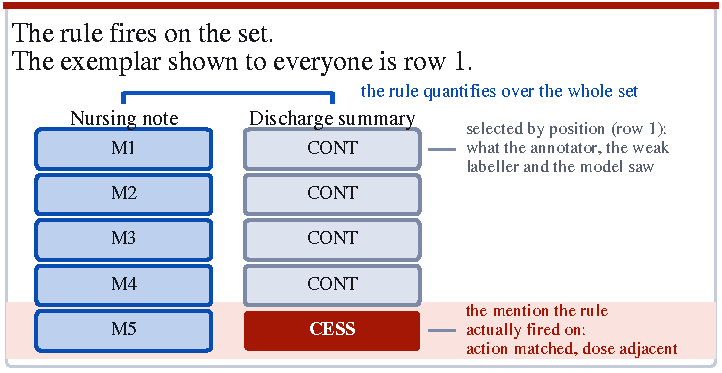
\includegraphics[width=0.88\linewidth]{figures/fig-exemplar.pdf}
\label{fig:exemplar}
\end{figure}

The second is the harm
head, which received no term in the training objective, so its reported
outputs are an untrained module's, invisible to an ablation delta and caught
only by checking a parameter's displacement from its own initialisation
(Chapter~\ref{ch:method}). The third is the row-level candidate split,
corrected to subject-level before any result in this document was generated
(Chapter~\ref{ch:method}): it contaminates whatever metric is computed
downstream of it without moving that metric's own diagnostics, and the check
is a subject-disjointness assertion between the two splits. The fourth,
scispaCy and medspaCy abandoned over dependency resolution rather than
evaluated and rejected, is a scope limitation rather than a metric-blind
defect: no reported number in this thesis depends on that choice, and no
check applies to it.

The multiplier that stage four carries is the weak labeller's positive rate on
the $299$-pair gold set over the pharmacist's base rate on those same $299$
pairs. Both terms are counted on the same rows.

\begin{figure}[!t]

\caption[The pipeline stage by stage]{The four stages whose reported number no
standard metric flagged, each with the check sensitive to what it hid. Stages
$1$ and $2$ reconcile in count and were never diagnosed. The scarlet carrier
marks the stage $3$ exemplar defect, which the weak labeller, the detector and
the pharmacist each saw; it records shared input, not cause. The architecture
row is categorical because no committed result file carries a number for it.}
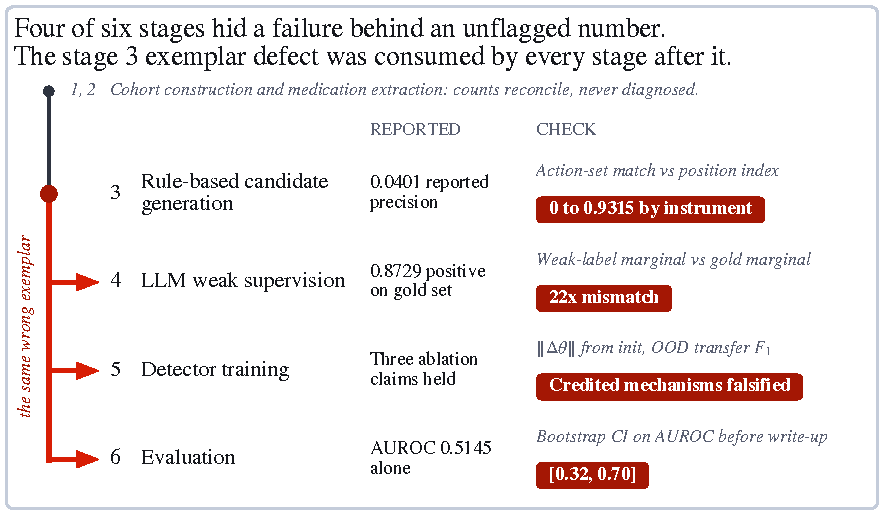
\includegraphics[width=0.98\linewidth]{figures/fig-pipeline-status.pdf}
\label{fig:pipeline-status}
\end{figure}

\section{The Finding}
\label{sec:intro-finding}

The pipeline does not work. This thesis establishes where it fails and why, by
running at each stage the control that separates a real result from an
artifact of the measurement; every stage failed its control, a statement made
once here so nothing later reads as a reveal. The cleanest single expression
of the failure is the decontaminated detector's operating behaviour on the
$253$ non-ambiguous pairs: at the configured threshold it predicts positive
for nearly the whole pool rather than ranking within it, and its ranking is at
chance rather than merely inaccurate, with Cohen's $\kappa$, the calibration
error, and the ensemble AUROC and its bootstrap interval reported at full
precision in Chapter~\ref{ch:results} (Section~\ref{sec:res-rq4},
Table~\ref{tab:decontam}) rather than restated here. Figure~\ref{fig:ceiling}
in Chapter~\ref{ch:results} carries the mechanism behind it: the largest
agreement any thresholded labeller could reach at the weak labeller's positive
rate on the $299$-pair gold set, against the pharmacist's base rate on those
same pairs, which is the marginal RQ2 below reports and RQ4 uses as a
precondition rather than an explanation. A TF-IDF
logistic-regression baseline on the $299$ annotated pairs ranks above both
neural configurations this pipeline produced, which is either surface-form
signal or small-sample noise and is not established either way
(Section~\ref{sec:res-rq4}). A null on twelve positives invites one obvious
reading, that the experiment was too small to see anything; the control that
answers it is a positive control run on the identical training and evaluation
harness, on a public benchmark rather than on this pool. Run on AG News under
an adjudication rule committed before the sweep, the resolved pretraining
benefit is $4.53$ accuracy points at convergence; the same harness, applied to
a clinical mortality task built for this control alone, returns a null,
$+0.0031$ (Section~\ref{sec:res-rq4}; Chapter~\ref{ch:discussion},
Section~\ref{sec:disc-null}). What that pairing licenses is that the harness
resolves a real difference at the sample sizes it was given; it says nothing
about the sensitivity of the twelve-positive contradiction evaluation itself,
which is fixed by that evaluation's own class counts and taken up next as a
screening test measured directly on the labellers this pipeline ran, rather
than as a resolution limit alone.


\section{Research Questions}
\label{sec:intro-rqs}

The project was organized around five questions: four about the stages of the
pipeline and one about the field that publishes pipelines like it. Each is
stated as it was posed, followed by the answer in one sentence. Evidence sits in
Chapter~\ref{ch:results}; the control designed for each stage is specified in
Chapter~\ref{ch:method} as a condition set before any result was seen.

\begin{description}

\item[RQ1. Candidate generation.] Can rule-based mining over paired clinical
notes yield a candidate pool with usable precision?
\emph{No: four rules enrich the pool to $12$ true contradictions in $299$
annotated pairs, a base rate of $0.0401$, and the evidence shown for each
candidate was selected independently of the evidence that triggered it, an
instance of the trigger-exemplar dissociation named in
Section~\ref{sec:intro-pipeline}. Section~\ref{sec:intro-contributions} below
gives the measured range at which that defect fired, and
Section~\ref{sec:intro-notclaim} states what it leaves of the $0.0401$
figure.}

\item[RQ2. Weak supervision.] Can a language model weak labeller substitute for
expert annotation at this base rate?
\emph{No: the weak labeller assigned the contradiction class to $261$ of the
$299$ annotated pairs against $12$ true positives, and every labeller tested
over-calls. Three local eight-billion-parameter models, run on an identical
prompt, over-call the candidate pool's confirmed rate by a multiplier from
$15.8196$ to $23.5959$ (Table~\ref{tab:overcalling}); the three already differ
from one another at this single point on any capability axis, and this
design has no compliant second point left to order them by scale. On a
public-text sweep run with the same three models and the same prompt, the
same mechanism tops out at $3.5000$ times (Section~\ref{sec:res-rq2}), so the
direction of the failure transfers across domains and its size does not.
Substitution fails at every local configuration measured; whether it fails
less at a scale this project could not run through a compliant channel is not
established.}

\item[RQ3. Architecture.] Do the proposed architectural components contribute
what they are credited with?
\emph{No, and the controls fire positively rather than by absence of evidence:
the authority parameters reported as learned finish at $0.5076 \pm 0.0006$ and
$1.0038 \pm 0.0010$ against initialisation at $0.5$ and $1.0$, the harm head's
outputs span $0.3977$ to $0.6096$, which is the range of an untrained sigmoid,
and on a second system built for this analysis, a single-seed randomised
control over the same role-label alphabet directionally loses to true role
labels by $0.3277$ nats with no significance claim attached, while an
arbitrary positional ordinal, a different feature rather than a randomised
version of the same one, beats both.}

\item[RQ4. Evaluation.] Can a labeller's capacity to show discrimination
against a gold standard be established before it scores a single pair, from
its marginal alone, and do the labellers this pipeline actually ran fail that
test?
\emph{Yes, and yes. Holding a labeller's flagged count and the gold
standard's confirmed count fixed fixes the best table of agreement that
marginal can ever produce, a ceiling that is arithmetic rather than a
property of what the labeller knows
\citep{feinstein1990paradoxes,cicchetti1990resolving,byrt1993pabak}, applied
here as a precondition rather than an explanation. Measured this way on
eight local labeller-and-basis rows, four could not have rejected the null at
$\alpha = 0.05$ at any outcome their own marginal permitted, because the
smallest one-sided $p$ value their marginal allows already exceeds it, and
four sit exactly on their marginal-implied ceiling, so their reported
agreement reports their flag rate and nothing else. The weak labeller
supplying the detector's training signal, at $261$ of $299$, is one of the
four that could not have rejected the null before it scored a single pair.
This bounds a thresholded decision only: a labeller that emits a continuous
score is not bounded this way, because the operating threshold can be swept,
and a model that flags most of a pool at one threshold can still rank the
pool perfectly at another. Section~\ref{sec:res-rq4} reports the eight rows
in full and states separately what the twelve-positive evaluation's own
class counts fix as a minimum detectable effect, a second and narrower
constraint on the same null.}

\item[RQ5. Practice.] Does published work audit the selection step upstream
of the model it evaluates, the one control this survey was built to measure?
\emph{Rarely, on that one control: on a $75$ paper corpus deliberately
enriched toward work that attends to selection, $4$ papers audit the
selection step under the strict reading and $14$ under the permissive one,
with both readings reported side by side and the gap between them named as a
coding ambiguity rather than resolved in the flattering direction. The survey
speaks to this one adjacent check; it is not evidence about whether published
work runs the other four controls RQ1 through RQ4 applied to this pipeline.}

\end{description}

RQ4 is the load-bearing check, in a stronger sense than a resolution limit
alone would give it. Without it, the weak labeller's marginal reads as one
more number a larger annotation budget might fix. With it, four of the eight
local rows this pipeline measured, including the row that actually supplied
the detector's training signal, could not have cleared the conventional
threshold at any outcome their marginal permitted, which means the ranking
null Section~\ref{sec:res-rq4} reports on the trained detector is not a
surprising failure to explain. It is the outcome the screening test already
predicted before the detector was trained. The twelve-positive evaluation's
own resolution limit, reported separately in Section~\ref{sec:res-rq4}, is a
second and narrower constraint on the same null; the two do not depend on one
another, and neither substitutes for the other.

\section{Contributions}
\label{sec:intro-contributions}

The methods applied in this thesis are not novel and the thesis does not claim
them. Negative controls come from epidemiology, and the positive direction is this thesis's adaptation of them, where that
literature is decades old \citep{lipsitch2010negative}. Randomisation based
sanity checks on learned components come from the saliency map literature
\citep{adebayo2018sanity}. Control tasks for probing classifiers come from work
that owns both the design and its conclusion \citep{hewitt2019control}. The
prevalence dependence of agreement statistics was described thirty-six years ago
\citep{feinstein1990paradoxes,cicchetti1990resolving}, and the adjusted
coefficient proposed in response removes the marginal sensitivity by removing
the marginal information \citep{byrt1993pabak}.
Chapter~\ref{ch:lit} attributes each of these to the work that owns it, and
this chapter's claim is about what they revealed when pointed at this pipeline.

What is new is the measurement on this pipeline and the fact that the controls
were actually run. Seven contributions follow, each stated at the size the
evidence supports, and one further result is reported separately below the
list because it does not meet the bar a contribution should meet. The twelve
confirmed contradictions bound only two of the strands below, the candidate
pool's precision and the detector's ranking nulls; the exemplar audit, the
survey, the convergence sweep, and the mortality control each carry their own
denominator, at the $165$-pair Rule 1 and Rule 2 pool, $75$ papers, $48$
runs, and $6{,}776$ admissions
respectively.

\begin{enumerate}
\item \textbf{Trigger-exemplar dissociation.} A mining rule whose predicate
quantifies over a candidate set while its exemplar selector picks by
position, with no assertion linking the two, silently corrupts the
annotator, the weak labeller, and the detector through the same wrong
exemplar; the one-line fix, asserting the exemplar belongs to the
predicate-satisfying set, would have caught it at no model cost, and on the
$165$-pair Rule 1 and Rule 2 pool it fired at a rate from $0$ to $0.4745$
depending on measurement (Figure~\ref{fig:exemplar},
Chapter~\ref{ch:results}).
\item \textbf{Two cheap, transferable checks: the degeneracy precondition
and sign provenance.} \emph{Degeneracy precondition:} a classifier that
predicts one class for nearly every input cannot exhibit a parity disparity,
so an audit reporting none on it reports its own operating point, not the
model; a pre-registered non-degeneracy bar plus a planted-gap positive
control, which aborts the run if a known disparity goes undetected, enforces
it. \emph{Sign provenance:} every disparity gap here was persisted through
an absolute value; retrofitting signed storage reproduced every prior value
exactly, with a maximum discrepancy of $0.0$, while reversing the sign of
seven of fourteen comparable drift slopes and flipping directional readings
already written down, a demonstrated true positive against this project's
own record.
\item \textbf{A measured null on clinical pretraining transfer, rather than
an underpowered one.} That pretraining loss poorly proxies downstream
performance is settled elsewhere at far larger scale
\citep{lourie2025scaling,feng2026tessera}; this $48$-run sweep only
replicates it. The contribution is the clinical null read as a measurement:
under an adjudication rule committed before the runs, the same harness
resolves $4.53$ points on AG News at $24$ epochs with seed standard
deviations at or below $0.0036$, and returns $+0.0031$ on the clinical task.
Section~\ref{sec:res-rq4} states what that figure does and does not rest on.
\item \textbf{A prevalence of practice measurement with released rows.} On
$75$ papers, $4$ audit the selection step under the strict reading and $14$
under the permissive one, across $502$ of $525$ quoted fields verified
against their sources, the rest coding absence with no quote to verify. A
blind second coder on $19$ overlapping papers gives $\kappa = 0.855$ at
$0.9474$ agreement on the permissive field and $\kappa = 0.730$ at $0.7895$
on null attribute handling; on the strict field both coders agree on all
$19$ papers, so $\kappa$ is \emph{undefined} rather than perfect.
\item \textbf{Prevalence mismatch contrast.} The same three local 8B models,
run with the same recovered prompt and greedy decoding, over-call on the
clinical pool by roughly sixteen to twenty-four times the base rate and on
public text by at most about three and a half times. The direction transfers
across domains and the magnitude does not. An earlier version of this
contribution attributed the magnitude to the pool's base rate rather than to
the model, then withdrew that attribution using a cell that varied the model
while holding the pool and the prompt fixed, at a scale beyond eight billion
parameters reached through a hosted channel. Every value from that channel is
now withdrawn from this thesis under the compliance action
Chapter~\ref{ch:method} records, so the cell that settled the attribution is
gone and the question it answered is open again rather than closed: whether
the sixteen-to-twenty-four multiplier belongs to the pool, the model, or both
is not established by any surviving cell, because every labeller whose result
survives the withdrawal sits at the same eight-billion-parameter scale. What
is unchanged by the withdrawal is narrower: a multiplier reported without
naming both the base rate and the model that produced it is uninterpretable,
and a later pre-registered test added the further condition that the prompt
must be named too.
\item \textbf{The misaligned-block arm and the global-positions confound
check.} Both are this thesis's own additions to a control-task design it
borrows, run on the second system, the provenance-conditioned encoder, not
the clinical contradiction detector. A hard block mask with zero trainable
parameters beats every learned attention-bias arm in the sweep by $0.1306$
nats, and an arbitrary positional ordinal carrying no provenance meaning
beats true role labels; restoring global positions on the shuffled-segment
setup recovers none of the segmentation gain, closing the confound that the
gain was a positionally handicapped baseline buying position back.
\item \textbf{What the controls cost.} Nobody reports this, so it is
reported here. The reconciled total across every control is $1216.4$ GPU
minutes over $79$ runs (Chapter~\ref{ch:discussion}); the raw log sums to a
smaller $661.4$ minutes, omitting the $555$-minute, $48$-run convergence
sweep entirely. The $34.9$-minute, $12$-run public-task episode it records
is additional compute, not a subset, so the total adds it along with the
clinical pretraining comparison's $612.3$ minutes over $17$ runs and the two
signed storage re-runs' $0.7$ and $13.5$ minutes. Person hours were never
logged, so the cost claim is compute only.
\end{enumerate}

\paragraph{A reported observation, not an eighth contribution.} On one
population with baseline disparity held fixed, two selection channels produce
demographic parity drift slopes of opposite sign, $-0.0078$ under one regime
and $+0.0118$ under the other, and a controlled simulator sweep inverts the
mapping rather than reproducing it. The pattern is reproducible and verified,
and it is retained in this thesis because it is what the sign-provenance work
in the second contribution turned up and because reporting a pattern that does
not fit is better practice than dropping it. It is not offered as a
contribution, because a contribution earns that billing by explaining
something, and this does not: no mechanism is offered, and none can be read
off the pattern, because interpreting a selection-dependent result requires
assumptions about the selection mechanism that are not available here
\citep{pfohl2025disaggregated,fogliato2020fairness}. Five mechanism claims
were proposed and refuted inside this project, and a sixth is deliberately
not being added. Chapter~\ref{ch:discussion} reports the pattern in full and
calls it what it is, an anomaly rather than a finding.

\section{What This Thesis Does Not Claim}
\label{sec:intro-notclaim}

This section sits in the introduction rather than only in the discussion,
because a reader is entitled to know the boundaries of a negative result
before reading the evidence for it, and it is one paragraph here because
Chapter~\ref{ch:discussion}, Section~\ref{sec:disc-limits} is where each
boundary is argued rather than asserted. This thesis does not establish that
the task is unsolvable, only that this pipeline does not solve it and that
the instrument used to say so could resolve a real effect where one existed;
it does not claim any of the controls as new methods, each is attributed
above to the literature that owns it; the survey is not a prevalence estimate
for clinical machine learning beyond its own deliberately enriched corpus,
and $\kappa$ on its strict cell is undefined rather than perfect; no
mechanism is claimed for the selection-channel anomaly and no subgroup harm
is demonstrated anywhere in this work; no rate is claimed from the project's
own correction record; the over-calling magnitude measured on this pool does
not generalise beyond it, a question narrowed rather than widened by the
compliance withdrawal Chapter~\ref{ch:method} records, which removed the only
cell that had varied model scale; and trigger-exemplar dissociation is not
evidence that the measured base rate is wrong, only that $0.0401$ is an upper
bound on annotation validity rather than a figure to be revised in either
direction.

\section{Organization of the Thesis}
\label{sec:intro-structure}

Chapter~\ref{ch:lit} reviews contradiction detection, clinical natural language
inference, evaluation under class imbalance, and the control literature this
thesis applies, with each control attributed to its source.
Chapter~\ref{ch:method} builds the cohort, the mining rules, the gold standard
and the detector, and states the control designed for each stage as a condition
before any result appears. Chapter~\ref{ch:results} reports the five findings,
the positive control and the survey, keeping the $299$ and $253$ denominators
separate throughout. Chapter~\ref{ch:discussion} takes up what each control
changed, the unexplained anomaly, sign provenance, and the threats to validity.
Chapter~\ref{ch:conclusion} restates the findings and names the work that
follows from the limitations.

% ============================================================================
%  Chapter 2. Literature Review
%
%  \input file for the MSU thesis. Requires booktabs, float and a natbib-style
%  citation command in the parent preamble. Bibliography: accord/thesis/refs.bib
%
%  Positioning chapter. It reports no results of this thesis. Every method the
%  thesis applies is attributed here to the work that owns it.
% ============================================================================

\chapter{Literature Review}
\label{ch:lit}

This thesis builds nothing new. It takes a pipeline whose shape is standard in clinical natural
language processing, rule-based candidate mining followed by language model weak supervision
followed by a purpose-built neural detector, and runs at each stage the control that separates a real
finding from an artifact of the measurement. The controls are borrowed, each credited again wherever
it appears later, so what this chapter has to establish is narrower than a conventional review: not
that a gap exists in the space of methods, but that a gap exists in the space of things that have
been checked.

The review runs along six threads: the clinical task itself, attempted far less often than its
importance suggests; weak supervision and label noise, where a single language model annotating a
rare class falls outside the theory the field's tooling rests on; evaluation under low prevalence, a
literature now thirty-six years old that this thesis applies rather than extends; controls and
construct validity, the methodological backbone; pretraining loss as a predictor of downstream
utility, settled recently at a scale this thesis cannot approach; and selection and stage-by-stage
auditing of pipelines. Each thread supplies a constraint the next has to respect, and each thread's
gap is named in the chapter's final section, which states what all six leave.

\section{Contradiction and Inconsistency Detection in Clinical Text}
\label{sec:lit-contradiction}

\subsection{The clinical problem the task inherits}

Adverse drug events are among the best documented inpatient safety problems, and the classic
incidence study of \citet{bates1995ade} established both their frequency and that a substantial share
are preventable. The transition out of hospital concentrates the risk: unintended medication
discrepancies are found at a large fraction of admissions \citep{cornish2005discrepancies} and at
discharge \citep{wong2008reconciliation}, discontinuity between inpatient and outpatient care affects
a meaningful share of discharged patients \citep{moore2003discontinuity}, adverse events after
discharge are frequently drug-related and preventable \citep{forster2003adverse}, the document meant
to prevent them is itself unreliable in content and timing \citep{kripalani2007deficits}, and its
timeliness is associated with patient outcomes \citep{li2013timeliness}.

Two features of that literature shape the computational formulation: the most common discrepancy
category is omission, a relation between a statement and the absence of one rather than a
disagreement between two statements, an asymmetry that does not survive translation into a
sentence-pair classification task; and the two sides of a cross-note comparison are not
interchangeable, since a discharge medication list is an instruction that will be acted on while a
nursing note records what was observed, and that relation has a direction that carries the
consequence.

\subsection{Formulations inherited from natural language inference}

Natural language inference classifies a premise-hypothesis pair as entailment, contradiction, or
neutral, and the large general corpora \citep{bowman2015snli,williams2018mnli} made it a standard
probe of sentence-level semantic competence. MedNLI \citep{romanov2018mednli} carried the task into
the clinical domain, using clinician-written hypotheses over patient-record premises, and remains the
closest established benchmark to the problem studied here. Later clinical resources moved toward
multi-evidence and numerical reasoning over structured trial documents \citep{jullien2023nli4ct},
still within a document rather than across documents written by different roles.

Contradiction detection as a task distinct from entailment was posed by
\citet{demarneffe2008contradictions}, whose typology separates negation, numeric, antonymy and
structural contradiction and whose central observation is that contradiction is rarer and worse
served than the symmetric three-way framing implies. In the biomedical domain
\citet{alamri2016corpus} built a corpus of potentially contradictory claims from cardiovascular
abstracts, a resource about published claims rather than care documentation. Work at document scale
is more recent: \citet{hsu2021wikicontradiction} learn contradiction-aware comparisons over sentence
pairs within a Wikipedia article, and \citet{li2024contradoc} annotate self-contradictions in long
documents and show that even strong large language models are unreliable on cases requiring context.

A separate body of work shows how inference models reach high benchmark accuracy without doing the
intended inference: hypothesis-only baselines recover much of the label signal
\citep{poliak2018hypothesis,gururangan2018artifacts}, lexical-overlap heuristics survive until probed
adversarially \citep{mccoy2019hans}, the pattern is characterised as shortcut learning
\citep{geirhos2020shortcut}, and the clinical analogue appears in imaging, where models key on
site-identifying artifacts \citep{zech2018generalization}. Those studies diagnose a model that scores
well; this thesis has a pipeline that scores poorly and needs to know whether the poor score is real.

\subsection{What has actually been built for the clinical case}

Very little, and the exception is instructive. \citet{li2015discrepancy} report an end-to-end hybrid
algorithm for medication discrepancy detection at Cincinnati Children's Hospital, comparing
structured discharge prescription lists against free-text notes for 271 patients in a Complex Care
Medical Home Program. Component performance on entity detection and attribute linkage is strong, but
combining stages drops precision, recall and $F$-measure to 71.5\%, 65.2\% and 68.2\% on discrepant
medications, well below the matched-medication figures.

Three properties of that setting explain why the numbers do not transfer, and they define the problem
this thesis takes on: one side of the comparison is structured rather than extracted from prose, the
cohort is a care-management program followed deliberately and so has a raised base rate, and the
comparison is anchored, since every prescription in the list is a candidate and no retrieval step can
silently bound recall. Remove all three, as a free-text-to-free-text comparison over an unselected
critical care cohort does, and detection becomes inseparable from retrieval: a candidate generator
sits in front of the model and caps its recall absolutely.

The extraction machinery for the medication half is mature: shared tasks established the entity and
attribute layer \citep{uzuner2010medication,henry2020n2c2}, negation handling has a standard solution
\citep{chapman2001negex}, and open tooling is available \citep{neumann2019scispacy,eyre2021medspacy}.
The layer above it is not: \citet{weiskopf2013quality} find completeness, correctness and
plausibility handled unevenly, and consistency across documents about one episode is a dimension the
reuse literature flags and the extraction literature does not target. The deployment literature is
clear about the consequence: \citet{vandersijs2006overriding} report override rates of 49\% to 96\%
for low-precision drug safety alerts, and \citet{ancker2017alertfatigue} find acceptance associated
with alert-stream complexity rather than workload, so a recall figure without the corresponding
precision says nothing about clinical usefulness.

\section{Weak Supervision and Label Noise in Clinical NLP}
\label{sec:lit-weak}

\subsection{Programmatic labelling and the assumption underneath it}

Distant supervision \citep{mintz2009distant} established the pattern of generating training labels
by projecting a structured resource onto unlabelled text and tolerating the resulting noise. Data
programming \citep{ratner2016dataprogramming} and its system realisation Snorkel
\citep{ratner2017snorkel} generalised this, allowing many noisy labelling functions and fitting a
generative model over their accuracies and correlations. The clinical track record is real:
ontology-driven weak supervision matches hand-labelled training data for entity classification
\citep{fries2021trove}, and cross-modal data programming speeds model development in medical imaging
by writing rules over an auxiliary text modality \citep{dunnmon2020crossmodal};
\citet{zhang2022wssurvey} survey the paradigm.

The guarantees require multiple sources whose errors are conditionally independent given the true
label, so that disagreement is informative and aggregation recovers a better label than any single
source. With one source, aggregation is the identity function and the generative model has no signal
to fit; this is the stated premise, not a subtlety buried in the proofs. What the literature does not
say is what to do when only one source is available and hand annotation is the resource being
economised on, which is what a single instruction-tuned model creates.

\subsection{The language model as annotator}

Since 2023 the default cheap labeller has been an instruction-tuned language model, on the strength
of results reporting that such models match or exceed crowd annotators on several classification
tasks \citep{gilardi2023chatgpt}. \citet{pangakis2023validation} give the corrective: any automated
annotation procedure must be validated against human labels on the same items, since performance
varies enough across tasks that a headline accuracy from one setting licenses nothing in another.
Calibration is a second problem, since language-model confidence values are not calibrated
probabilities without measurement \citep{guo2017calibration} and are sensitive to prompt construction
and the class priors it implies \citep{zhao2021calibrate}.

Label noise has its own literature. \citet{frenay2014labelnoise} survey classification under label
noise and separate the cases that matter: noise completely at random, noise depending on the true
class, and noise depending on the features. The distinction is load-bearing, because the strongest
noise-robust guarantees assume one of the first two, whereas an annotator with a systematically
shifted prior produces a corrupted marginal rather than symmetric noise. \citet{northcutt2021labelerrors}
show that even curated benchmark test sets carry pervasive label errors whose correction can reorder
published rankings, making the reference standard itself an object needing audit.

\subsection{Surrogate labels bias what is computed from them}

The most directly relevant result is \citet{egami2023surrogates}, who consider the now-common
workflow in which a language model annotates a document set that feeds a downstream statistical
analysis, and show that direct use of surrogate labels causes substantial bias and invalid confidence
intervals even at 80\% to 90\% surrogate accuracy. Their remedy, design-based supervised learning, is
a doubly-robust estimator combining surrogate labels with a smaller set of gold-standard labels,
giving valid inference without assuming the surrogate is good.

Two things follow, and only one is usually noticed. The headline is that high annotator accuracy is
not sufficient for a valid downstream conclusion, so reporting it is not a validation step. The
second is that the correction itself requires gold labels on a subsample, which the workflow that
used a language model to avoid annotation entirely cannot supply. Their estimand is a population
quantity in a social-science analysis rather than the training signal of a detector, and no work was
found mapping the result to the case where surrogate labels are the training targets themselves. What
transfers is the shape of the warning: accuracy on the annotator's own terms says nothing about the
validity of what is built on it.

\subsection{Counting is a different problem from classifying}

An over-calling annotator is, among other things, a bad prevalence estimator, and there is a
literature about exactly that. \citet{forman2008quantifying} formalises quantification, estimating
class prevalence rather than labelling individual members, and shows the classify-and-count estimator
is biased whenever true and false positive rates differ, which is always; his adjusted-count
correction inverts the relation using estimates of those rates. \citet{gonzalez2017quantification}
review the resulting family of estimators.

The relevance to weak supervision is direct and, in clinical natural language processing, largely
unremarked. When a weak labeller's positive rate differs from the base rate, the quantification
literature says both what the discrepancy means and what correcting it requires: estimates of the
labeller's true and false positive rates on the same distribution, which require gold labels. This
correction and the Egami correction therefore fail for the same reason in the same setting, worth
noticing before running the annotator rather than after.

\section{Evaluation Under Class Imbalance and Low Prevalence}
\label{sec:lit-metrics}

\subsection{Agreement statistics depend on prevalence}

Cohen's kappa \citep{cohen1960kappa} corrects observed agreement for the agreement expected by
chance under the observed marginals, a function of those marginals in ways that surprise readers who
take it for a corrected accuracy. \citet{feinstein1990paradoxes} set out the two paradoxes: high
observed agreement can coexist with a low kappa when the marginals are badly unbalanced, and
unbalanced marginals can raise rather than lower kappa; the companion paper
\citep{cicchetti1990resolving} works through the resolution and recommends reporting the marginals
alongside the statistic. \citet{byrt1993pabak} respond with the prevalence-adjusted bias-adjusted
kappa, an affine function of observed agreement, $\mathrm{PABAK} = 2p_o - 1$, which removes the
marginal sensitivity by removing the marginal information: it reports a rescaled observed agreement
under the name of a chance-corrected coefficient, so a system evaluated by PABAK on a set with twelve
positives is scored almost entirely on its behaviour on the negatives, and whether that is right
depends on the exchange rate between a missed contradiction and a false alarm, a clinical question
the papers in this thread do not address.

\subsection{The Matthews line and its limits}

The Matthews correlation coefficient, introduced for assessing secondary structure prediction
\citep{matthews1975mcc}, is the Pearson correlation between the binary prediction and the binary
label, computed from all four confusion matrix cells. \citet{chicco2020mcc} argue it should be
preferred to accuracy and $F_1$ under imbalance because it is high only when all four cells are
favourable, and \citet{chicco2021mccbalanced} extend the argument against balanced accuracy,
bookmaker informedness and markedness; \citet{powers2011evaluation} situates it among informedness
and markedness measures, and \citet{delgado2019kappa} conclude from kappa's behaviour under skew that
it should be avoided in favour of MCC.

Balanced accuracy, the unweighted mean of sensitivity and specificity \citep{brodersen2010balanced},
is the measure most often reached for when a prevalence-blind summary is wanted, and its implicit
weighting is the least often written down. Under heavy negative skew the ROC curve is dominated by
the majority class and can look acceptable while precision-recall behaviour sits at the no-skill
line, which is why \citet{saito2015prcurve} argue the precision-recall curve should be the primary
tool at high skew; both are reported in this thesis. Two areas under the curve computed on the same
cases are correlated, so their difference cannot be tested as though the samples were independent;
\citet{delong1988comparing} give the standard nonparametric treatment, used once here to compare a
seed ensemble against a single model. \citet{schaeffer2023mirage} make the parallel argument at
scale rather than prevalence, attributing emergent abilities in large language models to nonlinear
metric choices rather than to a change in model behaviour.

\subsection{Training under skew is not measuring under skew}

The class imbalance literature is large and mostly about fitting: resampling \citep{chawla2002smote},
characterisation of when imbalance actually hurts \citep{japkowicz2002imbalance}, a broad survey
\citep{he2009imbalanced}, cost-sensitive decision rules \citep{elkan2001cost}, loss reshaping in
several forms \citep{lin2017focal,cui2019classbalanced,cao2019ldam,menon2021logitadjust}, and
positive-unlabelled formulations \citep{bekker2020pu}. Their relevance here is bounded by a single
result: \citet{vandengoorbergh2022harm} show, in clinical risk prediction, that imbalance corrections
including undersampling, oversampling and SMOTE produce severe miscalibration without improving
discrimination as measured by AUROC, and that whatever sensitivity gain they deliver is available by
shifting the threshold instead. Such corrections move the operating point along a ranking; they do
not create ranking information.

The tools that address the measurement side sit outside that literature: decision curve analysis
\citep{vickers2006dca} evaluates a model across the threshold probabilities a decision maker might
hold, and cost-sensitive learning \citep{elkan2001cost} makes the exchange rate an explicit
parameter. Reporting guidance for clinical prediction models now covers machine learning explicitly
\citep{collins2024tripodai}, and several of its items, participant flow, outcome determination,
sample size justification and prespecified performance measures, are mechanical enough to check
before a results table exists.

\section{Controls and Construct Validity in Machine Learning Evaluation}
\label{sec:lit-controls}

This section describes the methodological backbone of the thesis, and everything in it is
borrowed; laying it out at length makes the attribution unambiguous. Each subsection names
the owner, states the design, and identifies the stage of this project it is applied to.

\subsection{Negative and positive controls in observational research}

\citet{lipsitch2010negative} formalised the negative control for observational epidemiology: a
noncausal association between exposure and outcome threatens any causal claim, so one tests for it
by finding an exposure known not to cause the outcome, or an outcome known not to be caused by the
exposure, and checking whether the analysis nonetheless produces an association. An association where
none can exist is evidence that the analysis is picking up confounding, recall bias, or a defect in
procedure, though the control does not identify which. A positive control runs the same analysis in
the opposite direction, on a case where an effect is already known to exist, so the result speaks
about the instrument rather than the question asked of it; \citet{lipsitch2010negative} do not
formalise this direction, and this thesis adapts their device to build one on the same terms. The
transfer to a machine learning pipeline is direct: replace the substantive input with one that cannot
carry the claimed information, hold everything else fixed, and see whether the reported effect
survives, evidence rather than an absence of it, because the control fires and produces a number
where the theory says there should be none.

\subsection{Randomisation tests for attribution}

\citet{adebayo2018sanity} apply the same logic to saliency maps: a model randomisation test
progressively randomises trained weights and asks whether the saliency map changes, and a data
randomisation test retrains on permuted labels and asks the same; some widely used methods produce
visually plausible maps independent of both, so those maps cannot be evidence about the model. The
design generalises past saliency to any component credited with contributing something: replace what
it consumes with something that cannot contain the credited signal and see whether the contribution
persists.

\subsection{Control tasks and selectivity}

\citet{hewitt2019control} supply the design the architecture control in this thesis is built on. A
probe trained to predict a linguistic property from a neural representation may succeed because the
representation encodes the property, or merely because the probe is expressive enough to memorise the
mapping. Their control task assigns random outputs to word types, trains the same probe on that, and
defines selectivity as the gap between linguistic and control task accuracy; common probing setups
have poor selectivity, dropout does not fix this for multilayer perceptron probes, and a more
selective representation layer can win despite lower raw accuracy. \citet{belinkov2022probing}
synthesises the literature that followed: probe accuracy alone identifies neither what a
representation encodes nor whether the model uses it, an ordinal or categorical feature a component
is credited with exploiting can be replaced with an arbitrary assignment of the same shape, and if
that assignment recovers the gain, the credited feature was not the source. The comparison must be
built into the design rather than added after a result looks suspicious, because a control chosen
after the fact is a different object.

\subsection{Leakage and measurement}

\citet{kaufman2012leakage} give the formulation, detection and avoidance of leakage in data mining:
the introduction of information about the target that should not legitimately be available. Their
detection advice is behavioural, since a model performing implausibly well relative to the task's
difficulty is the primary symptom; an auxiliary objective derivable from the model's own inputs is a
textbook instance, and the diagnosis is that the target is not independent of what the model already
has.

\citet{jacobs2021measurement} bring measurement modelling from the quantitative social sciences to
computational systems, and their framing covers the whole chapter: systems operationalise
unobservable constructs through observable proxies, and the gap between construct and
operationalisation is where harms and invalid conclusions originate. They give fairness-oriented
accounts of construct reliability and validity, arguing that disagreements about fairness definitions
frequently mask disagreements about the underlying construct. The question here is not whether a
detector reaches some score but whether what is scored, a rule-mined candidate pair judged by one
annotator against heuristic-selected evidence, is a measurement of clinical contradiction.

\paragraph{What this thesis takes, and what it does not claim.}
Table~\ref{tab:lit-controls} lists the instruments and their owners. Every row is a method
applied without modification to a new object. None is a contribution of this thesis, and the
Methodology chapter repeats the attribution at the point of use.

\begin{table}[H]
\caption[Controls and their literature sources]{Controls applied in this thesis and the work that owns each one.}
\label{tab:lit-controls}
\centering
\small
\begin{tabular}{@{}p{1.9in}p{2.1in}p{1.9in}@{}}
\toprule
Instrument & Owner & Stage it is applied to \\
\midrule
Negative control & \citet{lipsitch2010negative} & Candidate generation \\
Randomisation sanity check & \citet{adebayo2018sanity} & Architecture components \\
Control task and selectivity & \citet{hewitt2019control} & Architecture components \\
Leakage diagnosis & \citet{kaufman2012leakage} & Auxiliary training objective \\
Surrogate label bias & \citet{egami2023surrogates} & Weak supervision \\
Prevalence-dependent agreement & \citet{feinstein1990paradoxes} & Reported metrics \\
Positive control, adapted & \citet{lipsitch2010negative}, negative controls & Evaluation instrument \\
Construct validity framing & \citet{jacobs2021measurement} & The task definition \\
\bottomrule
\end{tabular}
\end{table}

\section{Pretraining Loss as a Proxy for Downstream Utility}
\label{sec:lit-loss}

A pipeline that fails can always be defended on the grounds that it was too small, and the
counter-argument requires knowing whether the evaluation instrument could have registered a
real effect, which makes the relationship between a training objective and downstream
performance directly relevant. The recent literature on it is unusually clear, and two
results carry most of the weight.

\citet{lourie2025scaling} conduct a meta-analysis of published scaling results and find that
predictable scaling, small-scale results extrapolating to larger scales, occurs in a minority of
cases, 39\% of the time by their count, because small variations in experimental setup change
scaling behaviour enough to matter: the conditions under which scaling laws hold are
uncharacterised, so an extrapolation is a hypothesis rather than a prediction.
\citet{feng2026tessera} settle the narrower question of whether pretraining loss predicts
downstream utility, at a scale no thesis can match: within a Barlow Twins framework for Earth
observation foundation models, across 395 controlled training experiments and 15 downstream tasks,
the correlation between pretraining loss and downstream performance has an absolute Pearson
coefficient below 0.2, a general result about self-supervised pretraining, obtained far from
clinical text, and stronger evidence on the general proposition than anything this thesis could
produce.

The consequence is a limitation on what may be claimed, adopted rather than resisted: the Results
chapter reports a convergence experiment on the same harness for this reason, and the Introduction
states what it licenses for the clinical null rather than offering it as a contribution to the
scaling literature.

\section{Selection, Pipelines, and Disaggregated Evaluation}
\label{sec:lit-selection}

The literature on disaggregated evaluation, and what it assumes about the selection mechanism behind
a dataset, bears on one unexplained anomaly this project reports; that literature and the anomaly it
governs are both treated at length in the Supplement rather than here, since neither is a claim about
this thesis's own contradiction detector.

\subsection{Stage-by-stage auditing of pipelines}

\citet{biswas2021fairpreprocessing} already do stage-level auditing: they study fairness introduced
by data preprocessing rather than by the classifier, evaluate 37 pipelines drawn from three sources
using causal fairness measures, and show how the local fairness of individual preprocessing stages
composes into the fairness of the pipeline as a whole. The difference from the present work is the
object audited, not the idea of auditing by stage: their metric, fairness against protected
attributes, is defined at every stage, whereas the quantity here is the validity of each stage's
evidential claim, whether a candidate pool contains the pairs it should, whether a weak labeller's
marginal is usable, whether an architectural component contributes what it is credited with, and
whether the evaluation could resolve an effect. These are stage-specific and not comparable to one
another, so they cannot be composed the way a fairness metric composes.
\citet{sculley2015debt} anticipate the general hazard, that system-level defects arise at component
boundaries rather than inside any one of them, without proposing per-stage checks.

\section{What Is Left}
\label{sec:lit-gap}

The six threads leave one opening, and it is not a methodological one: each establishes what has
been built, checked or settled elsewhere, at a scale or in a subfield this thesis borrows rather than
extends, and each stops at a version of the same edge, named below one thread at a time. No
cross-note, free-text-to-free-text medication contradiction system or benchmark was found, and the
gap sits earlier than modelling, in whether a candidate pool can be assembled whose members are the
right pairs at all. No protocol was found for a single language-model annotator at low prevalence
used as the training signal itself, and every available correction requires gold labels the workflow
was built to avoid. None of the agreement-statistics papers states, for a given evaluation set, the
exchange rate a chosen measure imposes between a missed positive and an avoided false alarm
\citep{feinstein1990paradoxes}. No published work applies the instruments of
Section~\ref{sec:lit-controls} together across a pipeline's successive stages. Neither scaling paper
addresses what a positive control should look like for a clinical task with only a handful of
confirmed positives, where the question is whether a single comparison has power at all, not whether
a trend is predictable. And neither the disaggregated-evaluation nor the stage-auditing literature
supplies a per-stage check on the validity of an evidential claim in a text pipeline.

What has not been done is to take one clinical pipeline, apply the appropriate control at every
stage, and report the outcome whichever way it falls. Each control is cheap and standard in the
subfield that owns it; none was run on this pipeline before this work. The interesting output is the
joint pattern rather than any single control result: whether failures at successive stages are
independent defects or one defect propagating, and whether a labeller's own marginal already settled
what its evaluation could show.

Put in one sentence, the question this thesis asks is narrower than the pipeline that motivates it:
whether a language-model weak labeller's positive rate, set against expert-confirmed prevalence under
an honest reading of ambiguous cases, predicts what a trained detector can then show, at a sample
size that resolves only large effects. Nothing that follows claims to resolve more than that, and
nothing that follows claims a method this chapter has attributed to someone else.

% ============================================================================
%  Chapter 3. Methodology  (Morgan State MS format)
%
%  \input file. Parent (main_msu.tex) supplies report/12pt, double spacing,
%  Times, booktabs, graphicx, float, amsmath, natbib and .
%
%  PROVENANCE. Every reported quantity comes from results/accord/VERIFIED_FACTS.json.
%  Configuration constants (hyperparameters, pre-registered thresholds, rule
%  parameters) are cited inline to the committed source that defines them.
%  Quantities in the legacy draft chapters with no entry in VERIFIED_FACTS.json
%  are not restated. This chapter reports no outcomes; outcomes are Chapter 4.
% ============================================================================

\chapter{Methodology}
\label{ch:method}

\section{What This Chapter Specifies}
\label{sec:m-overview}

This chapter describes the pipeline that was built and, for each stage, the control designed to
separate a real finding from an artifact of the measurement. A control is informative only if the
condition under which it would fire is fixed before the number arrives, so every control below is
written as a condition, and Chapter~\ref{ch:results} reports which conditions were met.

The pipeline has four stages and an evaluation layer. Stage one extracts a cohort of admissions from
MIMIC-III and, for each, a paired nursing note and discharge summary. Stage two mines that corpus
with four rules to produce a pool of contradiction candidates. Stage three labels the pool with a
local language model. Stage four trains a neural detector on those labels and scores it against a
pharmacist-annotated gold set. Each stage inherits the previous stage's defects, which is why the
controls are given stage by stage rather than collected at the end. Two absences are deliberate:
there are no results here beyond counts registered in the project's verified-fact file with a
producing artifact, and there is no attempt to present the design as intended rather than as it
ran, because a methods chapter documenting the specification instead of the implementation is the
failure this thesis is about.

\section{Data and Cohort}
\label{sec:m-data}

\subsection{Source, access and text handling}

All clinical experiments use MIMIC-III v1.4 \citep{johnson2016mimic}, a de-identified critical-care
database from one academic medical centre. MIMIC-III is credentialed data; access came through the
standard PhysioNet route under a data use agreement, and that agreement determined how the analysis
was arranged. Four tables are used: \texttt{ADMISSIONS} for admission and discharge timestamps,
\texttt{PATIENTS} for the subject identifier used in grouping, \texttt{DIAGNOSES\_ICD} for the
ICD-9 codes defining the cohort, and \texttt{NOTEEVENTS} for the notes with their category label
and chart date.

No clinical note text appears in this thesis, in any table, figure, appendix or released artifact,
and no admission or subject identifier is printed anywhere. Note-derived intermediate files live
outside the version-controlled tree and never leave the analysis machine, and the export script
scans candidate files for note-text markers and aborts rather than filtering on a hit. Sentence
pairs were, in several runs, also sent to hosted model APIs; Section~\ref{sec:m-ethics} states why
every result obtained that way has been withdrawn from this thesis rather than reported.

MIMIC-III notes are de-identified by an automated system that replaces protected health information
with bracketed surrogate tokens \citep{neamatullah2008deid}. That is not neutral for a model
reading a fixed-length prefix, because surrogates cluster at the head of a note where name, date,
service and identifier fields sit. A model truncating a discharge summary to its first few hundred
WordPiece tokens is therefore reading an administrative header for some unknown fraction of notes,
which is a property of the data representation rather than of the modelling.

\subsection{Cohort definition}

The primary cohort is heart failure, chosen because polypharmacy is the norm in this population and
the drugs involved, among them loop diuretics and anticoagulants, have narrow therapeutic windows
and documented harm when continued inappropriately. Admissions enter if any ICD-9 code matches the
prefix \texttt{428}; two secondary cohorts were built for a transfer test, sepsis under \texttt{038}
and acute kidney injury under \texttt{584}. A prefix match on a billing code is weaker than the
physiologic criteria a clinical study would use, since it over-includes admissions where heart
failure is a comorbidity and under-includes admissions where the condition was present but uncoded.

The only further clinical filter is a positive length of stay. Applying the prefix match alone
returns 13,608 heart failure admissions; after the length-of-stay filter 13,597 remain, of which
10,143 belong to distinct subjects. The two secondary cohorts move by the same filter from 6,265 to
6,253 admissions for sepsis and from 11,422 to 11,408 for acute kidney injury, removing 12 and 14
admissions respectively against 11 for heart failure, in every case under one percent of the cohort.

\subsection{Note roles}

The clinical hypothesis is that note types carry different institutional weight. A nursing progress
note recording that a diuretic was withheld is an account of what happened at the bedside; a
discharge summary instructing that the same diuretic be continued at a stated dose is an order
governing the patient after discharge. A disagreement between the two is asymmetric, because only
one of them is the document the patient and the receiving clinician act on.

A three-role partition adding a physician or admission note was tried and dropped: physician note
types in MIMIC-III are unevenly populated across the covered period, and requiring three roles at
once intersects three sparse conditions, so no configuration reached usable coverage. Dropping the
third role is a design cost rather than a nuisance, since a two-role partition cannot separate a
nursing-to-physician disagreement, a within-stay communication failure, from a nursing-to-discharge
disagreement, a failure that reaches the patient. The adopted partition maps
\texttt{discharge summary} to the discharge role, maps \texttt{nursing} and \texttt{nursing/other}
to the nursing role, and discards every other category. It finds 13,321 of the 13,608 heart failure
admissions with a discharge summary and 10,012 with a nursing note; the intersection carrying both
roles is 9,820 admissions, the figure this thesis prints throughout.

One note per role per admission is then selected. The nursing note is the one with the latest
\texttt{CHARTTIME} strictly earlier than \texttt{DISCHTIME}, the last documented bedside state
before the patient leaves. The discharge summary is the first row under a deterministic ordering by
\texttt{CHARTDATE} with the row identifier as tie-break, since \texttt{CHARTTIME} is null for every
discharge-summary row in MIMIC-III: these notes are written retrospectively and only a
\texttt{CHARTDATE} is recorded. That ordering restores determinism, not sub-day chronology, which
the resource does not contain. Two consequences constrain later claims. Every statement that the
nursing note came first rests on the selection rule rather than on a measured comparison, and any
filter searching for documentation written between the two notes at sub-day resolution has an empty
interval to search: at that resolution the intermediate-documentation hypothesis is untestable in
this resource rather than tested and rejected. Counting at date-level resolution instead is a
coarser but answerable question, and Section~\ref{sec:m-candidates} reports it directly.

This selection returns 9,783 admissions with a selected nursing note and 9,783 with a selected
discharge summary, for 19,566 note rows across 9,783 pairs in total, 37 fewer than the 9,820
admissions carrying both roles; the shortfall is entirely nursing-side. Holding the nursing role
means holding at least one note labelled nursing; being selectable means holding one whose chart
time is recorded and falls strictly before the discharge time. An admission whose nursing notes all
carry a null chart time, or all fall at or after discharge, therefore has the role and no selectable
note, while the discharge side applies no such condition and loses nothing. That is the cohort the
mining rules of Section~\ref{sec:m-candidates} run against. Figure~\ref{fig:cohort-flow} carries the
whole path: admissions selected by billing code, filtered on length of stay, reduced to those
carrying both note roles, and reduced again to one note pair per admission; the medication mentions
extracted from those pairs and the subset carrying an action class; the candidates the four mining
rules return after the temporal prefilter; and the pairs a pharmacist annotated. The terminal box is
the non-ambiguous evaluation core and the confirmed contradictions inside it.

\begin{figure}[!t]

\centering
\caption[Cohort flow from the source database to the evaluated sets]{The path
from the source database to the evaluated sets, with the count at each stage and
the exclusions recorded as counts. Two intermediate exclusions are not drawn
because no committed file records either as a count.}
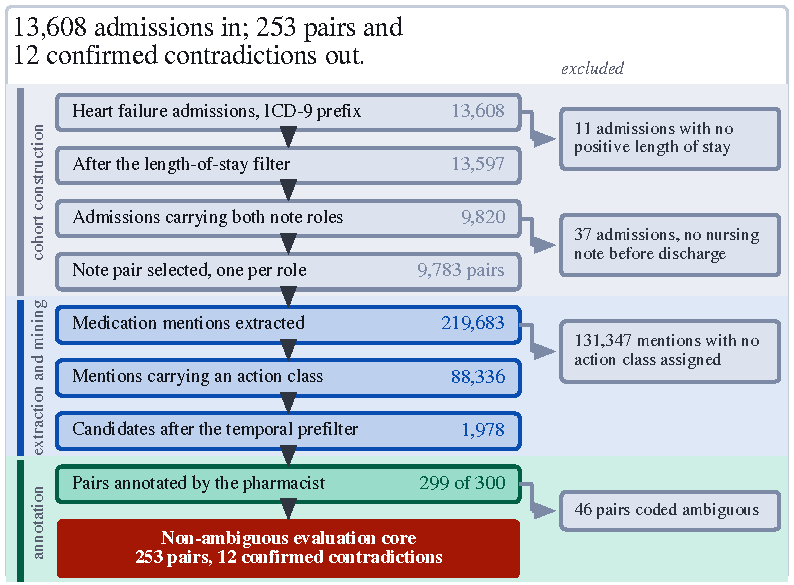
\includegraphics[width=0.88\linewidth]{figures/fig-cohort-flow.pdf}
\label{fig:cohort-flow}
\end{figure}

\subsection{Medication mention extraction and splitting}

Medication extraction is a mature task with strong published systems
\citep{uzuner2010medication,henry2020n2c2} and mature tooling
\citep{neumann2019scispacy,eyre2021medspacy}. This project used neither, after installation of both
failed against the pinned environment; the pipeline instead uses a dictionary extractor over a
general-purpose English pipeline. That is a limitation, not a considered choice.

The extractor uses four hand-written resources: heart-failure-relevant generic drug names;
abbreviation and brand-name expansions; spelling and formulation normalisations, so formulations of
one agent collapse to a single target; and regular expression alternations defining the action
classes cessation, continuation, initiation and dose modification, plus a separate negation
alternation. Matching is case-insensitive with word boundaries on both sides, applied after
expansion. Action classification operates on a window of three sentences, the previous, current and
next: the negation alternation produces a boolean over that window, the four action alternations
are applied in a fixed order and the first match determines the raw action, and negation then
rewrites the result, mapping continuation and initiation to cessation and cessation to
continuation.

Run over the 9,783 admissions the extractor returns 219,683 mentions across 9,732 unique admissions
and 70 distinct drugs, of which 88,336 receive an action classification and 131,347 do not. Fewer
than half of all mentions carry an action at all, which bounds how much of the corpus Rules 1 and 2
can ever reach, since both rules are defined entirely over the classified subset.

Three properties propagate downstream: the action is a property of the window and not of the drug
mention, so every drug named anywhere in the window gets the same label; first-match ordering makes
the classes non-exclusive in effect, since a window carrying vocabulary from two classes resolves
to whichever is tested first; and the negation rewrite is a hard flip with no scope model, where a
purpose-built context algorithm would model scope explicitly \citep{chapman2001negex}.

Two fields exist only in the rebuild: a numeric dose parser reducing a matched dose string to a
value and a canonical unit, converting within the mass family and leaving other unit families
incomparable since conversion needs drug-specific information the resource lacks, and a sentence
index and character offset on every mention, without which the defect in Section~\ref{sec:m-exemplar}
is enabled, since two mentions of the same drug in one note are otherwise indistinguishable rows.

Candidates concentrate within admissions and the patient population has repeat admissions, so a
row-level split would place candidates sharing a nursing note, a discharge summary, an admission or
a patient on both sides, since two candidates from one admission differ only in the drug at issue
while the surrounding text and documentation style are identical. Every split used here is instead
disjoint by \texttt{SUBJECT\_ID}, asserted in code rather than assumed:
\[
S_{\text{train}} \cap S_{\text{val}} = S_{\text{train}} \cap S_{\text{test}}
= S_{\text{val}} \cap S_{\text{test}} = \varnothing ,
\qquad
S_{\text{train}} \cup S_{\text{val}} \cup S_{\text{test}} = S .
\]
Patient-level grouping is the correct unit because it is the only unit guaranteeing no shared note
and no shared documentation episode. Row-level decontamination is weaker still, since a subject can
contribute one admission to the gold set and another to the weak-label pool, so the control
training pool of Section~\ref{sec:m-control-model} excludes, by assertion, every weak-label row
whose subject appears in the gold set.

\section{Candidate Generation}
\label{sec:m-candidates}

\subsection{Formulation}

True cross-note medication contradictions are rare, exhaustive human review of the cohort is
infeasible, and exhaustive machine scoring of all cross-note drug pairs is both wasteful and
statistically hostile. Candidate generation is the standard response: a cheap, high-recall,
low-precision rule set narrows the space to a pool a human or a model can examine. The rules are
not intended to be accurate, only transparent, so each candidate carries a reason, and enriching, so
the base rate inside the pool exceeds the rate outside it.

Let admission $a$ have a nursing note $N_a$ and a discharge summary $D_a$, with mention sets
$M(N_a)$ and $M(D_a)$. Each mention $m$ carries a normalised drug $\mathrm{drug}(m)$, an action
label $\mathrm{act}(m) \in \{\textsc{cess}, \textsc{cont}, \textsc{init}, \textsc{dose},
\textsc{unc}\}$, an optional numeric dose $(\mathrm{val}(m), \mathrm{unit}(m))$, a sentence
$\mathrm{sent}(m)$ and, in the rebuild only, a position $\mathrm{pos}(m)$. A candidate is a tuple
$c = (a, r, d, m_N, m_D)$, where $r$ indexes the rule, $d$ is the drug or drug pair at issue, and
$(m_N, m_D)$ is the exemplar pair, the single mention from each note presented as evidence. The
distinction this section turns on is between the trigger predicate $T_r(a,d)$, which decides
whether a candidate exists, and the exemplar selector $E_r(a,d)$, which decides what evidence
accompanies it. A correct implementation requires that $T_r$ holding implies $\mathrm{act}(m_N)$
and $\mathrm{act}(m_D)$ are the two actions that made it hold.

\subsection{The four rules}

Rule 1 fires when the same drug appears in both notes and the action sets disagree in a specific
direction. With $A_N = \{\mathrm{act}(m) : m \in M(N_a),\ \mathrm{drug}(m) = d\}$ and $A_D$ defined
analogously,
\[
T_1(a,d) =
(\textsc{cont} \in A_N \wedge \textsc{cess} \in A_D)
\;\vee\;
(\textsc{cess} \in A_N \wedge \textsc{cont} \in A_D).
\]
This is the canonical case: the nursing note records the drug as held and the discharge summary
orders it continued, or the reverse. The existential quantifier means the rule fires if some
mention on each side carries the required action, correct for a high-recall trigger and exactly
what makes exemplar selection non-trivial.

Rule 2 relaxes drug identity to pharmacologic class, so two different agents in one class, one
continued and one ceased across the notes, can be flagged as a substitution documented on one side
only. It uses a hand-written class dictionary covering the major heart-failure classes, plus a
guard that the drug sets on the two sides are not identical, which would return the candidate to
Rule 1. The dictionary is small relative to the pharmacologic space, is not derived from a standard
terminology such as ATC or RxNorm, encodes one author's judgement at its boundaries, and has no
mechanism for cross-class interactions.

Rule 3 fires when the same drug carries a parseable numeric dose in both notes, the doses reduce to
the same canonical unit, and they differ by more than a fixed fraction of the larger value:
\[
T_3(a,d) = \exists\,(m_N, m_D):\
\mathrm{unit}(m_N) = \mathrm{unit}(m_D)\ \wedge\
\frac{\max - \min}{\max} > \tau ,
\]
with $\tau$ fixed at $0.20$ in the mining implementation. The threshold is a judgement call
with no empirical derivation, it is not tuned, and it is not clinically grounded, since a given
proportional change in a statin dose and the same change in a warfarin dose are not comparable
events. Its exemplar selection is correct by construction, because the exemplar is the pair
achieving the largest proportional difference.

Rule 4 fires when a drug receives a cessation action in the nursing note and is absent from every
extracted mention in the discharge summary, classified or not:
\[
T_4(a,d) =
\bigl(\exists\, m \in M(N_a):\ \mathrm{drug}(m) = d \wedge \mathrm{act}(m) = \textsc{cess}\bigr)
\;\wedge\;
d \notin \{\mathrm{drug}(m) : m \in M(D_a)\}.
\]
This is the clinically most interesting rule and the weakest in evidence, since absence is not a
decision: a drug held at the bedside and never mentioned again may have been deliberately
discontinued and correctly omitted, or dropped by oversight, and the rule cannot tell them apart. It
also produces a structurally different input, since there is no discharge sentence to show and the
discharge side is a literal marker, so any difference in labeller or model behaviour on Rule 4 has
at least two explanations, clinical reasoning and a formatting response to a degenerate input,
which the design cannot separate.

Rules 3 and 4 exist only in the rebuild, since the reference extractor never parsed dose strings or
recorded positional information; comparison between rebuild and reference behaviour is therefore
restricted to Rules 1 and 2, which is what defines the defect-free stratum used in
Section~\ref{sec:m-control-rq1}.

Applied to the classified mentions, the four rules return a raw pool of 1,980 candidates before any
temporal check, split 886 from Rule 1, 203 from Rule 2, 521 from Rule 3 and 370 from Rule 4,
covering 1,205 distinct admissions. A temporal prefilter requiring a resolvable ordering between the
two notes drops the pool to 1,978 candidates, split 886, 202, 520 and 370, out of 1,068 admissions
carrying a usable date window and 643 carrying an intermediate note between the two selected notes.
Every candidate count elsewhere in this thesis is the post-prefilter figure, 1,978, unless stated
otherwise.

\subsection{Exemplar selection, and the defect in it}
\label{sec:m-exemplar}

The reference mining code for Rules 1 and 2 selects the exemplar by positional index into the
drug's mention group, taking the first row on each side, with nothing constraining those rows to
carry the actions that made the trigger true. If a discharge summary mentions a drug several times,
mostly continuation with one later cessation, while the nursing note has a single continuation
mention, the trigger fires on the continuation-cessation branch and the candidate is real by the
rule's own definition, but the positional selector returns a continuation row on the discharge side,
so the exemplar presented as a contradiction consists of two sentences in which the notes agree.

This is a methods matter rather than an incidental bug: the pharmacist annotated the exemplar pair,
the weak labeller read it, and the detector was trained on it, so wherever the selector failed, all
three reasoned about evidence that did not contain the conflict which caused the candidate to exist.
The defect was invisible because of an upstream schema decision rather than a typo: with no sentence
index and no character offset, two mentions of one drug in one note are indistinguishable rows, so
positional selection is not obviously different from any other choice, and there was no
representation in which the mention carrying the conflict could be expressed. This is configuration
and data-dependency debt in the sense of \citet{sculley2015debt}, a defect made unreachable by the
absence of the field that would have exposed it.

The rebuild selects, on each side independently, among only those mentions whose own action equals
the action required by that candidate's conflict branch:
\[
E_r^{\text{new}}(a,d) = \Bigl(\arg\min_{m \in C_N} \delta(m),\;
\arg\min_{m \in C_D} \delta(m)\Bigr),
\quad
C_X = \{m : \mathrm{drug}(m) = d,\ \mathrm{act}(m) = \rho_X\},
\]
where $(\rho_N, \rho_D)$ is the action pair required by the branch that fired and $\delta(m)$ is
the character distance from $m$ to the nearest dose-bearing mention in the same note. The tie-break
is a heuristic with a stated rationale and no validation: a mention adjacent to a concrete dose is
more likely to be a substantive instruction than a passing reference in an allergy or problem list,
and with no dose-bearing mention it falls back to the earliest qualifying sentence for determinism.
Because it chooses among mentions that already qualify it cannot reintroduce the original defect,
and whether it changes a clinical judgement was not measured.

\section{Weak Supervision}
\label{sec:m-weak}

\subsection{Labeller, pool and prompt protocol}

Training a supervised detector on a few hundred annotations containing a handful of positives is
not viable, so this project uses weak supervision: obtain approximate labels cheaply, accept that
they are noisy, and rely on the model to average over the noise \citep{ratner2017snorkel}. Since
2023 the dominant cheap labeller has been an instruction-tuned language model, on the strength of
results showing such models matching or exceeding crowd annotators on several classification tasks
\citep{gilardi2023chatgpt}.

The production labeller is Llama 3 8B \citep{grattafiori2024llama3}, run locally and presented with
each candidate's exemplar sentence pair and the identifier of the rule that generated it, asked for
a binary judgement plus a confidence value. The prompt is a fixed template with no demonstrations
and no chain-of-thought elicitation, and it names a conflict type before asking whether a conflict
is present. The labelled pool is the candidate pool minus the pairs put to the pharmacist, disjoint
at the row level by construction; Section~\ref{sec:m-data} explains why that was insufficient. The
weak-labelled candidate pool from this calibration join holds 1,679 rows before subject-disjoint
exclusion; removing the 291 rows whose subject also appears in an evaluation split leaves 1,388,
split into the 1,183-row training pool reported in Table~\ref{tab:m-strata} and used to fit the
detector, and a 205-row validation pool used only to monitor the training loss.

For the replication in Section~\ref{sec:m-control-rq2} the evaluation baseline's prompt was
recovered verbatim from the committed prompt table rather than rewritten, and reused unchanged
across models. It is not the deployed weak labeller's prompt, which the table does not contain, so
the replication reproduces the baseline configuration rather than the configuration that produced
the training labels; the deployed run and the same model's baseline-prompt replication differ by
$165$ positive labels across the full pool, a lower bound on the rows they disagree on (Section~\ref{sec:res-rq2}). Decoding is greedy at temperature zero
for the local models, so a model's label for a row is deterministic within a model. Generations that
do not parse are recorded in their own category and never defaulted to a class, which would otherwise
inflate a positive rate mechanically and silently.

\subsection{How \texttt{weak\_confidence} was derived}

The labelling stage emits a \texttt{weak\_confidence} field alongside each label. Across the
training pool and the audited rows it takes exactly two distinct values, one for each label class,
in a one-to-one mapping, so it is a deterministic function of the label and carries no information
about the labeller's uncertainty on any individual example.

The field was used in two places, both converting a label into a training-time intervention. As a
filter, the training code discards rows whose confidence falls below a threshold lying beneath the
field's minimum value, so the filter removes nothing while reading, in the code and in every
description of the pipeline, as a quality-control step. As a loss weight, the same field is
multiplied into the per-example loss, making it a label-conditioned reweighting rather than a
confidence weighting, in the direction that further downweights the already-dominant class. A
confidence value emitted by a language model alongside a label is not a calibrated probability and
should not be treated as one without measurement \citep{guo2017calibration,zhao2021calibrate}.

Weak labels are used only as training supervision here, never as ground truth, so any metric
computed against them measures agreement with the labeller rather than clinical correctness.
Validation of an automated annotation procedure against human labels on the same items is a
requirement rather than an option \citep{pangakis2023validation}, and the gold set of
Section~\ref{sec:m-gold} supplies those items.

\section{The Detector}
\label{sec:m-detector}

\subsection{Backbone, and what the running code contained}

The encoder is BioMedBERT (released as PubMedBERT) \citep{gu2021biomedbert}, selected over ClinicalBERT
\citep{alsentzer2019clinicalbert} on published benchmark performance, adapted with low-rank
adapters on the attention projections \citep{hu2022lora}. Each candidate's nursing and discharge
sentences are encoded, each truncated to a fixed prefix from the head of the sequence, which is
where Section~\ref{sec:m-data}'s observation about the de-identification header applies. The system
was specified as that backbone plus four purpose-built components: a cross-note difference encoder,
an asymmetric conditioning module, a pharmacological prior conditioning module, and a
guideline-grounded harm estimator, with three claimed contributions attached to them. What follows
describes the code that produced the results rather than the specification, per the correction
recorded as C4, one of the entries named but not reproduced in Appendix~\ref{app:corrections}.

The pharmacological prior module was deleted in the second version and replaced by a function
returning a fixed-length vector of zeros with two positions overwritten, one a danger multiplier
and one a normalised rule identifier. It has zero learned parameters, and the running code contains
no drug class table, no interaction table and no contraindication list.

The guideline-grounded harm estimator has no guideline corpus: its guideline bank is a single
randomly initialised parameter matrix cross-attended from one query, with no document collection,
index, retrieval step or text of any kind. More consequentially, the harm head and the explanation
head receive no loss term, since the objective is a weighted sum of only the contradiction loss and
the rule-type loss, so both heads are randomly initialised modules whose outputs are computed,
recorded and reported while their weights never move; the severity-ranking question was therefore
not tested, and any correlation between that head's output and a human danger rating measures an
untrained module rather than severity ranking.

The auxiliary rule-type head predicts the rule identifier that the prior-feature constructor writes
into the model's input, one linear layer apart in the same forward pass, so the task is a copy
operation. Auxiliary-label leakage of this shape belongs to a documented family
\citep{poliak2018hypothesis,gururangan2018artifacts,mccoy2019hans,geirhos2020shortcut}: an auxiliary
head whose target is derivable from its own input features is not an auxiliary task, and the
cheapest test is out-of-domain transfer rather than held-out accuracy \citep{zech2018generalization}.

The asymmetric conditioning module carries a two-element authority parameter initialised at the
pair of values later reported as discovered, applied to a cross-attention branch that is
immediately layer-normalised. Layer normalisation is invariant to a per-branch scalar rescaling of
its input up to the effect on its own affine parameters, so the normalisation removes most of what
the parameter does and the gradient reaching it is correspondingly small. The diagnostic that
follows is stated as a rule and applied in Chapter~\ref{ch:results}: for any parameter reported as
learned, publish its relative displacement from initialisation and a gradient-norm trace.

\subsection{Pretraining, and an untrained configuration}

Before supervised training the model was to be pretrained with a cross-note coherence objective,
discriminating genuine note pairs from mismatched ones. One configuration has a surviving run
record, with a frozen backbone; a wider configuration, meant to test whether trainable capacity
rather than architecture was the constraint, was never trained. The Stage 0 training script freezes
the backbone unconditionally with no code path that unfreezes any encoder layer, and the parameter
total attributed to the wider configuration is reconstructible only by counting a pooler module
that a forward and backward pass confirmed carries gradient flags and no gradient
(Appendix~\ref{app:corrections}, C54).

No claim of the form ``X was never trained'' may rest on the absence of a checkpoint, since a
checkpoint for the wider configuration does exist on a drive mount an earlier search did not reach
(Appendix~\ref{app:corrections}, R6); the claim here rests on the code path and the gradient check
alone.

\subsection{The defect-free control model}
\label{sec:m-control-model}

Because the detector carries documented defects, a null measured on it alone cannot be attributed
to the task. A second model was built as a control rather than a competitor, and it is deliberately
boring. The nursing and discharge sentences are concatenated with separator tokens, passed through
BioMedBERT, and the raw first-token hidden state feeds one linear layer producing one logit under a
binary cross-entropy objective. There is no rule feature, no authority parameter, no auxiliary
head, no harm head and no confidence reweighting, since any of those would reintroduce a defect the
control exists to rule out.

The training protocol is fixed and reported in full. The train and validation split is drawn by
subject with a dedicated split seed held fixed across runs, so variation between runs reflects
model stochasticity and not different training data, and the seed setter is called inside each
run's own process, one process per seed, so no session state carries across runs. Optimisation uses
AdamW at learning rate $2\times 10^{-5}$ with weight decay $0.01$, batch size 16, three epochs and a
maximum sequence length of 160 tokens, all fixed rather than swept.

Two floor baselines are trained on the identical pool and split so the comparison is like for like:
a majority-class predictor assigning every gold row a constant score equal to the training-pool
positive rate, and a TF-IDF representation with at most $5{,}000$ features feeding logistic
regression. The constant score yields an AUROC of exactly $0.5$ by construction, making it the
correct reference point for reading any AUROC near chance.

\section{The Gold Standard}
\label{sec:m-gold}

\subsection{Sampling and annotation protocol}

A stratified sample was drawn from the candidate pool, allocated across the four rules in
proportion to each rule's share of the pool (886, 202, 520 and 370 candidates for Rules 1 through
4), rounded to whole pairs and not oversampled toward any rule. The frame draws 134 pairs from Rule
1, 31 from Rule 2, 79 from Rule 3 and 56 from Rule 4, for 300 pairs total, the same sampling
fraction in every stratum to within rounding, and was fixed before annotation began. Proportional
allocation has a consequence Chapter~\ref{ch:results} relies on: under it, the gold sample's base
rate is an unbiased estimate of the pool's base rate, the denominator the over-calling ratios in
that chapter divide against. The returned annotation set has $n = 299$ pairs, one fewer than the
frame; the per-rule breakdown, 134, 31, 79 and 55, shows the missing row belongs to Rule 4, since
Rules 1 through 3 returned every sampled pair and Rule 4 returned one fewer than it was sent.

A single board-certified pharmacist annotated the sampled pairs, recording for each a three-way
label, contradiction, not a contradiction, or ambiguous; a free-text justification; a confidence
rating; and, for contradictions, an ordinal danger rating. The annotator saw the exemplar sentence
pair and the rule that generated the candidate, which is the same evidence the weak labeller and
the detector saw. Annotation ran in two passes separated by a two-week washout. The two-pass design
controls for within-session drift and fatigue, and that is all it controls for; it does not
establish inter-rater reliability, because there is one rater.

\subsection{The ambiguity category}

A pair was coded ambiguous when the presented evidence did not permit adjudication, rather than
being forced into a binary that would have converted an evidential limitation into a label
indistinguishable from a genuine negative. The category has a cost in the evaluation layer, handled
by reporting both readings rather than choosing one: ambiguous pairs are retained as negatives in
the primary stratum and excluded in the power calculation the project originally referenced, which
is why Section~\ref{sec:m-stats} reports the minimum detectable effect under both denominators, and
no result here is reported under only one treatment of the ambiguous rows.

\subsection{What this design can and cannot establish}

A reliability claim previously attached to this gold set is retracted here rather than in a
footnote, because the retraction concerns the instrument. The project reported a Cohen's $\kappa$ of
$1.000$ between two independent pharmacist judgement instruments, which were in fact the binary
contradiction label and the ordinal danger rating: a pair that is not a contradiction has no danger
by definition, so the agreement between a positive label and a positive danger rating is an identity
guaranteed by construction \citep{cohen1960kappa} and measures nothing about annotator reliability.

The honest statement is that this study has one annotator, a two-pass protocol with a washout, and
no established inter-rater reliability; a second annotator would be the highest-value single
addition to the work, and its absence is a first-order limitation on every conclusion resting on the
gold labels.

Intra-rater agreement is not a fallback here. The two-pass protocol reduced within-session drift and
fatigue in a single rater; it did not produce two comparable sets of judgements, since the
annotation file stores one final label per pair and the second pass overwrote the first rather than
being retained beside it. No artifact in this project keeps the pass-one and pass-two labels
separately, so a figure computed after the fact would have to be re-annotated from scratch to exist
at all. The reliability of the gold standard is therefore not a missing number the project failed to
report but one the retained record cannot produce, and every clinical result in this thesis rests on
a single-rater instrument with no inter-rater or intra-rater agreement statistic attached to it.

\begin{table}[H]
\caption[Evaluation strata and their sizes]{Evaluation strata, their sizes, and their positive counts.}
\label{tab:m-strata}
\centering
\small
\begin{tabular}{lrrl}
\toprule
\textbf{Stratum} & \textbf{$n$} & \textbf{Positives} & \textbf{Defined by} \\
\midrule
Gold, all annotated pairs & 299 & 12 & Ambiguous rows retained as negatives \\
Gold, defect-free subset  & 134 & 6  & Rules 3 and 4 only \\
Decontaminated evaluation & 253 & 12 & Ambiguous rows excluded \\
Weak-label training pool  & 1,183 & \multicolumn{2}{l}{Positive rate 0.8521} \\
\bottomrule
\end{tabular}
\apanote{The defect-free subset is fixed by rule membership before any score is computed. The training pool's positive rate is the weak labeller's marginal on the rows surviving subject-level exclusion, and it is the reference against which any agreement figure on weak labels must be read.}
\end{table}

\section{The Controls}
\label{sec:m-controls}

Each subsection states one control as a condition: what would have to be true for the corresponding
reading to survive. Every condition is written before any number in Chapter~\ref{ch:results} is
available to the reader. None of these controls is novel, and none is claimed as a contribution.

\subsection{RQ1: is the pool's precision an estimate or an upper bound?}
\label{sec:m-control-rq1}

\textbf{Condition.} If the exemplar selector agrees with its own trigger on substantially every
action-conflict candidate, the pharmacist judged the evidence that caused the candidate to exist,
and the measured precision estimates the pool's precision. If it does not agree, the measured
precision is an upper bound on the validity of the annotation exercise, and the direction of the
bias is not determinable from the data collected.

The audit instruments both selectors and records, for every action-conflict candidate, whether the
positional exemplar's action pair matched the pair required by the branch that fired, and whether
the corrected selector changed the chosen rows. Two quantities follow, an agreement rate and a
change rate, and they are not the same quantity: a candidate can change exemplar on one side while
the old exemplar happened to be correct on the other. The second half of the control is structural
rather than measured. Rules 3 and 4 have no positional selector, so the gold pairs drawn from them
form a defect-free stratum fixed before any model score exists, and every detection metric in
Chapter~\ref{ch:results} is reported on that stratum as well as on the full set. If the two strata
disagree, the exemplar defect is doing work; if they agree, it is not.

\subsection{RQ2: is the labeller's error noise or prior?}
\label{sec:m-control-rq2}

\textbf{Condition.} If a weak labeller's error were noise, its marginal would approximate the true
base rate and its mistakes would spread across classes. If its marginal sits far above the base
rate, the error is a prior shift, and no downstream aggregation removes a shifted marginal:
aggregation frameworks assume noise that is conditionally independent across sources given the true
label and rest on having multiple sources whose errors are not aligned \citep{ratner2017snorkel}.
One source with a systematic prior shift is outside that regime.

Three controls bear on this. First, ordering: the base rate must be estimated on a small
human-labelled sample before any weak labels are generated; this project produced the pharmacist
annotations after the weak labels, inverting the only ordering in which the mismatch would have
been actionable, reported here as a methods failure rather than repaired retrospectively.

Second, replication across labellers: if over-calling is a property of one model it will not
survive a change of model, but it will if it is a property of the task presentation. The
replication reruns the recovered baseline prompt unchanged over the full pool with three local
instruction-tuned models, \texttt{llama3:8b}, \texttt{granite3.3:8b} and \texttt{qwen3:8b}, served
through Ollama at temperature zero, with unparseable generations kept in their own category. Third,
a domain control: if the magnitude of over-calling generalises, a comparable labelling task on
public non-clinical text will show a comparable ratio, and if only the mechanism generalises the
ratio will be materially smaller while the direction persists, which governs what may be claimed.

\subsection{The marginal feasibility gate}
\label{sec:m-feasgate}

A thresholded labeller's flag count and the gold standard's confirmed-positive count fix, before any
score is compared, the largest attainable agreement and the smallest attainable one-sided
hypergeometric $p$ that marginal permits: placing every confirmed case inside the flagged set gives
the best table that marginal could produce. A labeller whose floor sits above the read-at threshold
could not have rejected the null however it behaved. The bound covers a hard, thresholded decision
only; a scored labeller can sweep its threshold and rank well regardless of flag rate, so this says
nothing about a ranking metric. Applied to every hard-label marginal this thesis prints, it was added
after the hosted results were withdrawn, unlike the controls above, specified before any result was
seen. The ceiling is the prevalence-and-bias problem of \citet{feinstein1990paradoxes} and
\citet{cicchetti1990resolving}, corrected by \citet{byrt1993pabak}; no novelty claim attaches to the
floor.

\subsection{RQ3: do the architectural components contribute what they are credited with?}
\label{sec:m-control-rq3}

\textbf{Condition.} A component credited with exploiting a semantic property must beat an arbitrary
substitute that carries no such property. If the arbitrary substitute matches or exceeds the
semantic feature, the credited mechanism is not the operative one, and the control has fired
positively rather than by absence of evidence. This is the control-task logic developed in the
probing literature by \citet{hewitt2019control}, applied here rather than proposed.

The arbitrary-substitute control operates on a second system in this project that conditions a
shared additive attention bias on document provenance. Seven arms were trained at three seeds each,
and three further arms at a single seed, on masked language modelling over packed multi-document
bundles, with segment order shuffled so role is decorrelated from position within the bundle: no
bias; a T5-style relative position bias; a misaligned block bias; an ALiBi-style distance bias; true
role labels; an arbitrary segment ordinal carrying no provenance meaning; and a fixed hard block
mask, the encoder analogue, under masked language modelling, of the intra-document mask
\citet{zhao2024seqcomposition} apply during causal decoder pretraining, the same mask construct but
a different training objective, disclosed here rather than treated as a reproduction. Two
comparisons are fixed in advance: true role labels against a randomised relabelling drawn from the
same alphabet, the control task in the sense of \citet{hewitt2019control}, and true role labels
against an arbitrary positional ordinal, a competing hypothesis rather than a control. The
misaligned block arm is a second control, holding the number of blocks fixed while destroying their
alignment with document boundaries, closing the reading that any coarse blocking of the attention
matrix would do.

One control, a single global derangement applying one fixed permutation to every bundle, is
deliberately not used and must not be confused with the randomised relabelling reported in
Chapter~\ref{ch:results}: since the bias table is a free matrix over role pairs, the model would
simply learn the permuted table and the loss surface is isomorphic, fixing the result at the
uncorrupted value by construction. It was implemented, recognised as powerless, and guarded against
in code, because a control that cannot fail is worse than no control.

A third control, the anisotropy control, addresses the representation rather than the mechanism.
The pretraining collapse was originally explained by clinical homogeneity, the claim that notes
within an institution are too similar for a coherence objective to separate genuine from mismatched
pairs, though nothing in the pipeline had measured note similarity. The control instead tests
whether the collapse follows from representational geometry in the encoder, passing deliberately
unrelated non-clinical sentences through the identical frozen extraction path and comparing mean
pairwise cosine similarity against matched and mismatched clinical pairs; text this similar to
itself under the same extraction weakens the homogeneity explanation without asserting the two
conditions are statistically identical, and Chapter~\ref{ch:results} reports a Welch test that
rejects exact equality.

\subsection{The degeneracy precondition}

\textbf{Condition.} Demographic parity compares the predicted-positive rate across groups, so a
classifier that predicts one class for nearly every input has the same predicted-positive rate in
every group by construction and cannot exhibit a parity disparity, whatever the underlying data. An
audit that reports no disparity on such a classifier is therefore reporting its own operating point,
not a property of the model or of the data it was run against. This is the degeneracy precondition:
a check on the validity of a parity-style audit over a binary classifier, checkable before the audit
runs. It is a precondition, not a general result about fairness metrics, and beyond what the rest of
this chapter already reports it establishes nothing about this thesis's contradiction detector.

The precondition is enforced by two mechanisms, run in order and both before the audit produces any
substantive measurement. First, a pre-registered non-degeneracy bar: the reference classifier must
clear a minimum AUROC of $0.65$, a predicted-positive rate strictly inside the interval $0.05$ to
$0.50$, and a precision lift over the base rate of at least $1.5$, all on the validation split and
all asserted in code before the sweep begins; if any of them fails, the driver exits and the sweep
does not run. Second, a planted-gap positive control, which runs immediately afterwards and checks
that the audit can detect a disparity known to be present: a known logit shift is injected into one
group's scores on the full population with no selection filtering, and the audit code must recover
it, the bootstrap interval on the demographic parity gap must exclude zero and the four-fifths ratio
must fall below its threshold with an interval upper bound below one. If the audit cannot recover a
gap placed there deliberately, every downstream number is void, and the experiment driver aborts
rather than reporting them. The precondition also applies retrospectively to an earlier audit in
this project and fails there, which is why no subgroup harm is demonstrated or claimed anywhere in
this thesis.

\subsection{RQ4: is the detector's null real?}

\textbf{Condition.} A null result is evidence only if the instrument that produced it can be shown
to resolve an effect of comparable size where one is known to exist, and only if the evaluation had
enough power to see an effect at all. Two local checks answer this together: the minimum detectable
effect for the evaluation's own sample size (Section~\ref{sec:m-mde}), and a positive control that
runs the same pretraining-effect instrument on a task where the effect is known to be present, its
outcome bound in advance to a written decision rule.

The proxy under test is whether a difference in self-supervised pretraining, measured as a loss
gap, predicts a difference in downstream discrimination. On the clinical side the comparison runs
on a task built for this control rather than on the contradiction detector: in-hospital mortality
predicted from a bundle of a patient's first 48 hours of notes, evaluated on $6{,}776$ held-out
admissions holding $570$ positives, a different task and cohort from the $253$-pair
contradiction evaluation. The comparison there is a from-scratch encoder against a
domain-pretrained encoder under a matched fine-tuning protocol at three seeds each. The two arms do
not share a seed set, so the comparison is unpaired and no per-seed difference is meaningful, and
one from-scratch run carries no recorded split lineage against the other five, so
Chapter~\ref{ch:results} reports the three-seed gap as primary and the two-seed gap over the
lineage-pinned runs alone beside it. On the public side the same comparison runs on AG News across
four arms, a pretrained BERT encoder against three from-scratch encoders at three smaller parameter
scales, with exact parameter counts given in Chapter~\ref{ch:results}.

One threat has to be answered before the public comparison can serve as a control: in the initial
sweep every arm trained for the same short budget with no per-arm tuning, so a gap between
pretrained and from-scratch arms could measure training budget rather than pretraining. The
convergence sweep instead gives every arm four budgets, each with its own complete schedule,
reported at the final epoch rather than by validation-based checkpoint selection, at three seeds per
cell, for $48$ runs and $555$ minutes of compute. The decision rule in Table~\ref{tab:m-prereg} was
committed to the project repository at commit \texttt{b048829}, before the sweep started, and
applied by the analysis notebook without being edited after the first result landed.

\begin{table}[H]
\caption[Pre-registered decision rule for the control]{Pre-registered decision rule for the pretraining positive control, committed before the
sweep was run.}
\label{tab:m-prereg}
\centering
\small
\begin{tabular}{p{0.14\linewidth}p{0.38\linewidth}p{0.40\linewidth}}
\toprule
\textbf{Outcome} & \textbf{Condition at the longest budget} & \textbf{Consequence} \\
\midrule
A & Gap of at least $3.0$ accuracy points between the largest from-scratch arm and the pretrained
    arm, and the two arms' one-standard-deviation bands do not overlap
  & The instrument has a verified positive control. The clinical null may be read as a measured
    null. \\
\addlinespace
B & Gap below $3.0$ accuracy points, or the ordering is not resolved across seeds
  & The positive control fails. The clinical comparison reverts to an experiment too insensitive to
    see anything and must be written that way. \\
\addlinespace
Inconclusive & Gap in the range $2.5$ to $3.5$ points, or the bands touch without overlapping
  & Neither A nor B may be asserted. Report the budget curve as the finding and state that the
    control is unresolved at this compute scale. \\
\bottomrule
\end{tabular}
\apanote{The rule also forbids resolving a boundary case by adding seeds until it moves, which is optional stopping. It does not decide whether pretraining helps on the clinical task; it decides only whether the public comparison is sensitive enough to serve as a control, and the two questions must not be merged. The thresholds shown are configuration decided in advance, not results.}
\end{table}

\subsection{Base-rate comparison for the low-prevalence metrics}

\textbf{Condition.} Balanced accuracy, PABAK, $\kappa$ and MCC depend on prevalence as well as on
discrimination, so a value of any of them is uninterpretable without the value the same statistic
takes for a trivial predictor on the same margins. No prevalence-dependent metric is reported alone
here. Each appears beside the value achieved on identical confusion-matrix margins by a
majority-class predictor and by a constant-positive predictor, and an ordering among systems is
claimed only if the bootstrap interval on the difference excludes zero.

This is applied literature, not a contribution: the prevalence dependence of chance-corrected
agreement is set out by \citet{feinstein1990paradoxes} and \citet{cicchetti1990resolving}, the
prevalence-adjusted correction by \citet{byrt1993pabak}, the case for MCC over $F_1$ under
imbalance by \citet{chicco2020mcc}, the dependence of $\kappa$ on marginals by
\citet{delgado2019kappa}, and the balanced-accuracy case by \citet{brodersen2010balanced}.
Precision-recall summaries are preferred to ROC summaries where the positive class is very rare
\citep{saito2015prcurve}, and both are reported here. A quantity stored as an absolute value
supports no directional claim, whatever the magnitude, because the storage discards the sign the
claim would need.

\subsection{RQ5: the survey coding instrument}

\textbf{Condition.} A survey of practice is evidence about practice only if the coding rule is
fixed, applied uniformly, and reported under both the strict and the permissive reading of every
contestable boundary. Reporting only the reading that supports the thesis is the failure the survey
exists to expose.

The instrument distinguishes two audits a paper may perform. A model audit examines a trained model
for disparities across groups within the analysis pool. A selection audit examines the filtering
step itself for differential retention across groups, against a denominator existing prior to
filtering. Inclusion requires all three of: health, clinical or biomedical data about people; at
least one disaggregated performance or outcome metric broken out by a demographic or socioeconomic
attribute; and enough methods detail to determine what cohort the metric was computed on. Papers
are excluded when they are commentary, position or review articles with no empirical evaluation,
when they report no disaggregated metric, when the data is not health data, when the methods are
too thin to identify the cohort, or when the full text is not retrievable.

Queries were issued against machine-readable interfaces (NCBI E-utilities for PubMed and PubMed
Central, the arXiv Atom API, and ACL Anthology volume indexes), so the search is reproducible by
re-running the recorded query strings. Screening runs in three stages: an automated title and
abstract screen logging its exact exclusion rule for each record; a full-text retrieval quota
ranking records passing stage one by a pre-specified keyword-density score and advancing them until
the budget is met, with records below the quota logged as screened rather than silently dropped;
and a full-text screen read against the three inclusion criteria. The corpus reaching coding
contains $n = 75$ papers.

The primary coding of a selection audit is strict: a paper counts only if it compares the group
composition, or the retention rate, of the retained cohort against a denominator existing prior to
filtering, or otherwise directly tests the filter for differential retention; a demographics table
or a flow diagram of total counts excluded does not qualify, since neither has a denominator. A
second, permissive column counts any comparison of retained group composition against any external
or source figure, including census statistics or the parent database before filtering; it is a
strict superset of the strict column, enforced in code, and both readings are reported everywhere.
Every coded field requires a verbatim quote and a section location, checked by a verification
script against the source text by exact string match, and a quote that fails to match is rejected
and its field forced to unclear.

Three limitations bound what the instrument can measure. Each paper was coded once by the primary
coder under a shared written rule set; a blind second coder independently re-coded a deterministic
subsample of nineteen papers, the basis for the agreement statistics reported in
Chapter~\ref{ch:results}, and no agreement figure is claimed for the other fifty-six. Second,
inclusion criterion two requires a disaggregated metric, so every included paper audits a model on
its pool by construction: the count of papers coded as auditing a model on the pool equals the count
of included papers, both $75$, so the cross-tabulation of model audit against selection audit
degenerates to a single row, and the keyword-density ranking enriches the corpus toward
fairness-forward work, against the direction of the finding rather than toward it. Third, the coded
question is only whether a paper audits the selection step upstream of the model it evaluates. It is
not the exemplar-correctness check, the weak-label marginal check, the architecture randomisation
control, or the positive control for evaluation sensitivity, and the survey measures none of them,
so the corpus supports only the prevalence of this one adjacent practice, not a claim about whether
the field runs the controls that would have caught this pipeline's own failures.

\section{Statistical Procedures}
\label{sec:m-stats}

\subsection{Bootstrap intervals and correlated AUROC comparison}

Interval estimates on AUROC and average precision are nonparametric percentile bootstraps over the
evaluation rows \citep{efron1994bootstrap}. The main control uses $10{,}000$ resamples at a fixed
generator seed of $20260806$; the decontamination analysis uses $10{,}000$ resamples at seed
$42$. Seeds
are recorded so that every interval computed here is reproducible to the digit. Degenerate resamples are handled
explicitly rather than by imputation: with few positives a resample can contain none, in which case
AUROC is undefined, so such resamples are discarded and do not count toward the requested total.
The count is reported beside an interval only where that interval's own artifact stored it, which
is not everywhere: among the intervals printed in Chapters~\ref{ch:results}
and~\ref{ch:discussion}, those computed for the control model carry a recorded count of valid
resamples, in every case the full $10{,}000$ requested, while the decontaminated ensemble's
intervals and the Matthews correlation intervals store no count of either kind. Where no count is
stored, none is quoted; read those intervals as computed over the requested resamples less an
unrecorded number of degenerate draws. A separate bootstrap of the defect-free stratum, not
printed in this thesis, does record its discards, $20$ of $10{,}000$, a rate of $0.002$, the only
direct measurement of that rate in this work.

Two systems scored on the same rows produce correlated ROC curves, so an unpaired comparison
overstates the variance of their difference. Comparisons between the control model and the
detector, and between individual seeds and the detector, use the DeLong test for correlated areas
\citep{delong1988comparing}, which estimates the covariance of the two areas from the same subjects
and returns a $z$ statistic and a two-sided $p$ value. The implementation is committed with the
analysis code released alongside this thesis, and the per-comparison outputs, including the standard
error of the difference, are written to the control report rather than recomputed in prose.

\subsection{Minimum detectable effect}
\label{sec:m-mde}

The sensitivity of the evaluation is a property of the evaluation set rather than of any model, so
it belongs in the methods. Under the null of no discrimination, the standard error of an AUROC
estimate with $n_+$ positives and $n_-$ negatives is approximated by
\[
\mathrm{SE}_0 = \sqrt{\frac{n_+ + n_- + 1}{12\, n_+ n_-}} ,
\]
with $\alpha = 0.05$ and power $0.80$ throughout. This
null-standard-error approximation is reported in Table~\ref{tab:m-mde} for reference, but it is not
what the table's minimum detectable AUROC column uses. That column follows the full
\citet{hanley1982meaning} procedure, which evaluates the sampling variance of the AUROC estimator at the
candidate value $a$ itself rather than at the null, and finds the smallest $a$ such that
$(a - 0.5) / \sqrt{\mathrm{Var}(a)} \geq z_{1-\alpha/2} + z_{1-\beta}$ by search, since
$\mathrm{Var}(a)$ depends on $a$. The full procedure was reimplemented and rerun for this thesis,
and the values below are that recomputation's output (Appendix~\ref{app:corrections}, R9).
Table~\ref{tab:m-mde} evaluates this under
each treatment of the ambiguous rows and on the defect-free stratum
(Figure~\ref{fig:power}, Chapter~\ref{ch:results}).

\begin{table}[H]
\caption[Sensitivity of the evaluation by stratum]{Sensitivity of the evaluation under each treatment of the ambiguous rows.}
\label{tab:m-mde}
\centering
\small
\begin{tabular}{lrrrr}
\toprule
\textbf{Stratum} & \textbf{$n_+$} & \textbf{$n_-$} & \textbf{$\mathrm{SE}_0$} & \textbf{$\mathrm{AUROC}_{\min}$} \\
\midrule
Gold, ambiguous excluded & 12 & 241 & 0.0856 & 0.7355 \\
Gold, ambiguous retained & 12 & 287 & 0.0852 & 0.7350 \\
Defect-free subset       &  6 & 128 & 0.1210 & 0.8058 \\
\bottomrule
\end{tabular}
\apanote{$\mathrm{AUROC}_{\min}$ is computed by the same procedure that also drives the marker positions in Figure~\ref{fig:power}. Values are rounded to four decimal places. These figures bound what the evaluation could have seen and are not results about any model. They also state the limit of the thesis's negative claim: nothing here can establish that the task is unsolvable, only that this pipeline does not solve it at a sensitivity this coarse.}
\end{table}

\subsection{Seed variation and the standard-deviation convention}

The subject-disjoint control and the decontaminated retrain each run at three seeds. The seed controls model initialisation, dropout and data loader
shuffle order. It does not control the train and validation split, which is fixed once by a
separate split seed, so the spread across seeds reflects training stochasticity and not resampled
training data. That is a deliberate narrowing: it makes the error bars interpretable as run-to-run
variability and means they exclude sampling variance.

Error bars reported as $\pm$ are standard deviations across those three seeds, not standard errors
and not confidence intervals. The convention has to be stated because it is not uniform in the
underlying artifacts. The subject-disjoint control computes the across-seed standard deviation with
$\mathrm{ddof} = 1$, the sample convention, while the decontamination analysis computes it with
$\mathrm{ddof} = 0$, the population convention. At three seeds the two differ materially, so every
reported spread in Chapter~\ref{ch:results} carries its convention explicitly, and no spread
computed under one convention is compared against a spread computed under the other.

Two further reporting rules follow from documented defects in the earlier work. No standard
deviation is emitted over fewer than three genuinely independent runs, where independence means the
seed setter ran inside the run and the row was produced by that run rather than pasted from an
earlier one. And a reference row in any comparison table must be produced by the same script and
protocol as the rows it is compared against; where that is not true, the comparison is reported as
directional with no significance claim attached. Finally, every quantity in
Chapter~\ref{ch:results} maps to the committed artifact that produced it, and that mapping is
reproduced in the register released with the analysis code rather than asserted
(Appendix~\ref{app:provenance}).

\section{Data Use, Ethics, and Compliance}
\label{sec:m-ethics}

\paragraph{Note text, and third-party transmission.} During this project, sentence pairs extracted from MIMIC-III notes were sent to hosted large
language model services in several runs. PhysioNet's guidance of 24 September 2025,
\emph{Use of MIMIC Data with Large Language Models and Online Services}, states that the
Credentialed Data Use Agreement prohibits sharing access to the data with third parties including
sending it through APIs or using it on online platforms, and that MIMIC data must not be stored or
retained by third-party LLM services, with locally deployed models strongly recommended instead.
Every result obtained through a hosted service has been withdrawn from this thesis: no figure,
table or number reported in any chapter derives from any such transmission, and the numeric
provenance gate enforces this rather than leaving it to prose. The model comparisons this thesis does report
were produced by models served locally on the analysis machine, which is the route that guidance
recommends. Whether the withdrawn transmissions were consistent with the agreement is a
determination for PhysioNet and for the institution rather than one this thesis makes, and no
conclusion on it is asserted here. The full record of what was sent, through which route, and when,
is retained in the project's correction record and in the committed run artifacts, and is available
to either on request.

\paragraph{Storage and compute outside the repository.} Credentialed files, including a file joining
note sentences to weak labels, were at one point held in the author's institutional cloud account
and have since been consolidated under credentialed-only local storage; no script in the repository
reads that account.

\paragraph{The annotator, and credentialed access.} The gold standard was produced by one
board-certified pharmacist, who read each pair on the author's screen, in the author's presence, and
gave a judgment the author recorded; no file was transferred, printed or photographed, and nothing
was retained. The annotator does not hold PhysioNet credentialed access, and the written protocol
recorded neither that status nor this arrangement, which is described so that it can be assessed.

\paragraph{Re-identification and small cells.} No re-identification was attempted and nothing was
joined against MIMIC-III at the patient level. Subgroup results are one-way marginals only. Small
cells, some below ten observations, are reported without suppression and marked unpowered.

\paragraph{Clinical status, and code contribution.} Nothing in this thesis has been validated for
clinical use or supports deployment in any care setting. The analysis code is released, with one
gap: the deployed weak-labelling run cannot be repeated, because its script and prompt were not
committed. That run produced $1{,}425$ positive labels among the $1{,}679$-row weak-labelled pool,
which subject-disjoint exclusion narrows to the $1{,}183$-row training pool of
Table~\ref{tab:m-strata}, and the $261$ of $299$ marginal Chapter~\ref{ch:results} reports, so those
numbers cannot be regenerated by anyone.

% ============================================================================
%  Chapter 4. Results. \input file for main_msu.tex; requires booktabs, float,
%  graphicx, amsmath, natbib and \apanote. Bibliography: accord/thesis/refs.bib
%
%  PROVENANCE RULE: every numeric value below is registered in
%  results/accord/VERIFIED_FACTS.json, reported at the precision of that
%  register or rounded to four decimal places. A quantity the register does not
%  contain is stated qualitatively instead. Nothing is carried forward from an
%  earlier draft.
% ============================================================================

\chapter{Results}
\label{ch:results}

This chapter reports the measurements taken at each stage of the pipeline, one
section per research question, in the order the stages run: the reading a
competent evaluation would produce, the control designed to separate that
reading from an artifact of measurement, and what the control returned.

Three evaluation sets appear throughout and they are not interchangeable.
Table~\ref{tab:denoms} fixes them. Every metric below carries its denominator, and
a quantity that is a ratio of two registered counts is written as that ratio, for
example $12/253$.

\begin{table}[H]
\caption[The three evaluation sets]{The three evaluation sets used in this chapter.}
\centering
\small
\begin{tabular}{lrrrl}
\toprule
\textbf{Set} & \textbf{$n$} & \textbf{Positives} & \textbf{Negatives} &
\textbf{Definition} \\
\midrule
$G_{299}$ & 299 & 12 & 287 & all annotated pairs, ambiguous counted negative \\
$G_{253}$ & 253 & 12 & 241 & non-ambiguous pairs, ambiguous dropped \\
$G_{134}$ & 134 & 6  & 128 & Rule 3 and Rule 4 stratum, defect free \\
\bottomrule
\end{tabular}
\apanote{$G_{299}$ is all annotated pairs; $G_{253}$ excludes the ambiguous pairs; $G_{134}$ is the defect-free stratum from the control report. The 46 ambiguous pairs are the difference between the two negative counts, $287 - 241$. $G_{134}$ is a subset of $G_{299}$ and holds half of the 12 confirmed contradictions.}
\label{tab:denoms}
\end{table}

A spread reported as $\pm$ or as SD in this chapter is a standard deviation
across three seeds, not a standard error and not a confidence interval
(Section~\ref{sec:m-stats}). That standard deviation follows two conventions, because the underlying
artifacts use two: the decontamination
sources compute it at $\mathrm{ddof} = 0$, the population convention, and the
control, convergence and ablation sources compute it at $\mathrm{ddof} = 1$,
the sample convention. Each table below states which convention its own spreads
use, and no spread computed under one convention is compared against one
computed under the other.

\section{Candidate Generation}
\label{sec:res-rq1}

Can rule-based mining over paired notes yield a candidate pool with usable
precision? No. More useful is that the pool's measured precision bounds the
validity of the annotation exercise rather than the pipeline's quality.

\subsection{The pool and its base rate}

A board-certified pharmacist annotated 299 candidate pairs: 12 contradictions,
241 not contradictions, 46 ambiguous. The base rate is $12/299$ on $G_{299}$,
$12/253$ on $G_{253}$ and $6/134$ on $G_{134}$. The majority-class baseline has
average precision $0.0401$ on $G_{299}$ and $0.0448$ on $G_{134}$, the no-skill
lines for every average precision in this chapter. A pool at a base rate near four percent is not itself a failure,
because rule-based mining is a recall device and a low-precision pool is its
expected output. What fails is what the precision figure is then used to justify.

\subsection{Per-rule yield and precision}

The candidate pool itself is dominated by one rule: of the 1,978 post-prefilter candidates,
886 come from Rule 1, 202 from Rule 2, 520 from Rule 3 and 370 from Rule 4
(Section~\ref{sec:m-candidates}), so Rule 1 alone supplies close to half the pool. Pharmacist
precision, measured on the 299-pair gold sample, does not track that share. Table~\ref{tab:rule-precision}
gives the size of each rule's gold stratum, the pharmacist's true-positive rate on it, and ACCORD's
predicted-positive rate on the same rows.

\begin{table}[H]
\caption[Per-rule precision and predicted-positive rate]{Per-rule gold stratum size, pharmacist precision, and ACCORD's predicted-positive rate.}
\label{tab:rule-precision}
\centering
\small
\begin{tabular}{lrrr}
\toprule
\textbf{Rule} & \textbf{$n$} & \textbf{Pharmacist precision} & \textbf{ACCORD predicted positive} \\
\midrule
1, direct action conflict & 134 & 2.24\% & 97.01\% \\
2, drug class conflict    & 31  & 9.68\% & 96.77\% \\
3, dosage conflict        & 79  & 5.06\% & 97.47\% \\
4, discharge-side absence  & 55  & 3.64\% & 74.55\% \\
\bottomrule
\end{tabular}
\apanote{The four strata sum to 299. The ACCORD column is the contaminated released run of Table~\ref{tab:marginal} ($134 \times 0.9701 + 31 \times 0.9677 + 79 \times 0.9747 + 55 \times 0.7455 \approx 278$). A rule is a mining mechanism, not a clinical category: the pharmacist's failure-mode coding of the 12 confirmed contradictions returns 7 omissions, 3 dosage conflicts, 1 drug substitution and 1 class conflict, spread across all four rules rather than confined to Rule 4, whose gold stratum contains 2 of the 12.}
\end{table}

Table~\ref{tab:rule-precision} shows pool volume and hit rate moving in
opposite directions: Rule 2 has the highest pharmacist precision despite the
smallest gold stratum and pool share, and Rule 1 the lowest despite the
largest, so no single rule accounts for the pool's overall base rate.
ACCORD's predicted-positive rate is insensitive to that more-than-fourfold
spread in true precision across Rules 1 through 3, and drops only for Rule 4,
the rule with no discharge-side mention to score, consistent with the
calibration failure of Section~\ref{sec:res-rq2} rather than with
rule-sensitive discrimination. Combined, Rules 3 and 4 account for 134 of the
299 pairs and 6 of the 12 confirmed contradictions, so the positives are
spread across the rule set rather than concentrated in one rule.

Grouping by mechanism rather than by rule number, Rules 1 and 2 together
account for $165$ pairs with $6$ positives, a rate of $0.0364$; Rules 3 and 4 together account for
$134$ pairs with $6$ positives, a rate of $0.0448$. A Fisher exact test on that $2 \times 2$ table
gives an odds ratio of $0.805$ at $p = 0.7725$, achieved power is $0.0576$, and the smallest
absolute rate difference detectable at $80\%$ power is $0.0895$, more than twice the overall base
rate. The two mechanism groups are indistinguishable at this sample size, which is not the same as equal.
The per-rule reading stops at Table~\ref{tab:rule-precision}. A ranking statistic computed inside a
single rule would rest on a handful of confirmed positives with no committed interval to bound it,
so none is reported for a rule on its own.

\subsection{The exemplar selection defect}
\label{sec:r-exemplar}

Each candidate reached the annotator as one nursing sentence paired with one
discharge sentence. For the two action-conflict rules the discharge sentence was
taken from the first row of the matched-mention frame rather than the row
carrying the conflict that triggered the candidate. For a large minority of
action-conflict candidates the annotator therefore judged a sentence pair that
did not exhibit the conflict the prompt asserted was present.

Two measurements of how often the defect fired exist on the $165$ pooled Rule 1
and Rule 2 candidates, and they disagree, so both are reported. The first
reconstructs the exemplar from a mentions-table snapshot, calibrated against
what the pharmacist actually saw at $0.8934$ nursing-side and $0.9508$
discharge-side fidelity, not perfectly, because Section~\ref{sec:m-exemplar}
establishes that the exact original row order cannot be recovered: 137 of the
165 candidates resolve, 28 do not, and among the 137, 65
carried a discharge sentence that did not exhibit the conflict, a wrong rate
of $0.4745$. The second uses
a true key join instead of a reconstruction, exact where it applies but
applying to far fewer rows: only 23 of the 165 candidates carry a usable join
key, and on that subset the exemplar is correct on all 23, a wrong rate of 0.
If the reconstruction's rate of $0.4745$ were the true
rate and joinability were independent of correctness, the probability of drawing $23$
joinable rows and finding all $23$ correct would be $0.5255^{23}$, which is about
$4$ in ten million. The two measurements are therefore not two ends of one interval.
They are mutually exclusive unless joinability is strongly confounded with
correctness, and that confound is the load-bearing assumption behind keeping both
numbers. It is plausible on its face: a row carries a usable join key when
the pipeline's own bookkeeping about it was intact, the bookkeeping the
selector defect corrupts. That assumption is stated here, left untested, and
an attempt to test it is reported as inconclusive rather than as a result.

The two-by-two is stark: of the $23$ rows the key join resolves, $23$ are correct,
against $72$ correct and $65$ wrong among the $137$ the reconstruction resolves.
It is not a test of association: correctness for the $23$ was assessed by
the key join and for the $137$ by the reconstruction, so no row is measured by
both. The hypothesis such a table would reject is the conjunction of two claims,
that joinability is unrelated to correctness and that the two instruments share
an error rate; the second is already denied, since the reconstruction's
fidelity is calibrated against what the pharmacist saw while the key join is
asserted exact. A comparison across instruments of unequal known fidelity cannot
attribute its difference to the thing being studied. The rival reading generates
the same table and points the other way: rows that reconstruct badly may be
called wrong by the reconstruction rather than by the defect, making joinability
a proxy for reconstructability and $0.4745$ the artifact.

So the $23$ key-joined rows are not a random subsample of the $165$, and that is the whole of
what the table supports. It is reported without a $p$ value and is not a member of the
hypothesis family Section~\ref{sec:r-multiplicity} enumerates; a $p$ value was briefly
attached and counted there, and C90 records why both were wrong. The confound remains
unfalsifiable from the retained artifacts, which is a weaker and more accurate position than a
confirmation. One of these two numbers is still wrong and this thesis still does not know
which. Neither is discarded, and neither should be quoted alone. A
separate join, across all four rules rather than Rule 1 and 2 alone, matches
the $299$-row annotated sample to the rebuilt candidates table on $35$ rows;
that is a different operation with a different denominator, not a third
reading of the same exemplar-correctness question.
Figure~\ref{fig:exemplar} in Chapter~\ref{ch:intro} draws the mechanism the two
measurements are measuring. The rate at which the trigger-set slot and the
positionally indexed slot actually disagreed on the Rule 1 and Rule 2 gold
stratum ranges from $0$ to $0.4745$ depending on measurement, and a rate over a
population does not belong welded to a picture of a single case, so the figure
carries no number.

The measured consequence does not depend on that rate. Rules 3 and 4 cannot
exhibit the defect: Rule 3 selects the maximum-difference dose pair, and Rule 4
has no discharge sentence to select, because the drug is absent from the
discharge summary by construction. That yields $G_{134}$, and
Section~\ref{sec:res-rq4} reports two scores on that stratum: the defect-free
control model's, and ACCORD's contaminated released run rescored on the same
pairs. What it does not report is the decontaminated ACCORD ensemble on
$G_{134}$, because no per-pair score from the decontaminated retrain was
retained for those rows. The restriction does not move the conclusion and it
widens the intervals, as a stratification down to 6 positives at a minimum
detectable AUROC of $0.8058$ has to. The figure this defect bounds is an upper
bound on annotation validity, not an estimate of pipeline quality, and the
direction of the bias is unknown.

\section{Weak Supervision}
\label{sec:res-rq2}

Can an LLM weak labeller substitute for expert annotation at this base rate? No.
Every local labeller tested over-calls on the same pairs, by roughly fifteen to
twenty-four times the confirmed rate at eight billion parameters, already
enough review burden to matter for anyone judging how much of a pipeline
like this still needs a human check. Whether that multiplier falls
further at frontier scale was tested through a hosted API and the result is
withdrawn (Section~\ref{sec:r-frontier}); this chapter does not establish
whether the failure attenuates with capability or bottoms out at eight billion
parameters.

\subsection{The marginal}

On the 299 annotated pairs the weak labeller called 261 pairs contradictions and
the pharmacist called 12. Table~\ref{tab:marginal} puts the three marginals on
the one denominator where all three were recorded. Weak supervision of this kind
is defended on the grounds that the noise averages out \citep{ratner2017snorkel},
and that defence assumes noise conditionally independent across sources given the
label; one source whose error is a shifted marginal falls outside the regime.

\begin{table}[H]
\caption[Predicted-positive counts by source]{Predicted-positive counts on the 299 annotated pairs.}
\centering
\small
\begin{tabular}{lrl}
\toprule
\textbf{Source} & \textbf{Called contradiction} & \textbf{Denominator} \\
\midrule
Pharmacist (gold)                  & 12  & 299 \\
Llama 3 8B weak labeller           & 261 & 299 \\
ACCORD, released per-pair decision & 278 & 299 \\
\bottomrule
\end{tabular}
\apanote{The ACCORD decision column is three-valued; 15 rows carry the value \emph{ambiguous}. The 261 and the 278 count two different columns produced by two different systems on the same 299 rows and are not two readings of one quantity. The ACCORD row is the contaminated released run; the decontaminated retrain appears in Section~\ref{sec:res-rq4}.}
\label{tab:marginal}
\end{table}

$261$ against $12$, on identical inputs, is the finding.
\citet{pangakis2023validation} argue that an automated annotation procedure must
be validated against human labels on the same items; those items existed
before the labelling run, and the comparison was not made.

Three local 8B labellers were each run over the pool and the gold set, and the
over-calling ratio, the positive rate divided by the gold base rate of
$0.0401$, was measured for all three with zero unparseable responses.
Table~\ref{tab:overcalling} carries every over-calling ratio this chapter
reports, together with the positive rate and the count each rate is measured
on, so measurements taken on different sets are not mistaken for readings of
one quantity.

\begin{table}[H]
\caption[Over-calling ratios by labeller and evaluation set]{Every over-calling ratio this chapter reports on the candidate pool and on $G_{253}$, by labeller, evaluation set, positive rate, and the count the rate is measured on.}
\label{tab:overcalling}
\centering
\small
\begin{tabular}{@{}p{1.55in}p{1.15in}rrr@{}}
\toprule
\textbf{Labeller} & \textbf{Evaluation set} & \textbf{Positive rate} & \textbf{Ratio to $0.0401$} & \textbf{$n$} \\
\midrule
\texttt{llama3:8b}     & Candidate pool                    & 0.9470 & 23.5959 & 1,679 \\
\texttt{llama3:8b}     & $G_{299}$, gold set                & 0.9532 & 23.75   & 299   \\
\texttt{granite3.3:8b} & Candidate pool                    & 0.7219 & 17.9863 & 1,679 \\
\texttt{granite3.3:8b} & $G_{299}$, gold set                & 0.7425 & 18.5    & 299   \\
\texttt{qwen3:8b}      & Candidate pool                    & 0.6349 & 15.8196 & 1,679 \\
\texttt{qwen3:8b}      & $G_{299}$, gold set                & 0.6187 & 15.4167 & 299   \\
Llama 3, deployed weak labeller & Candidate pool & $1425/1679$ & 21.1473 & 1,679 \\
\bottomrule
\end{tabular}
\apanote{Each ratio divides a positive rate by the unrounded $12/299$ gold base rate, so recomputing from the printed $0.0401$ will not reproduce these ratios exactly. The first six rows are three local labellers on the candidate pool and the gold set; the seventh, the deployed weak labeller, differs by prompt (Section~\ref{sec:m-weak}). The $15.8196$ to $23.5959$ range quoted elsewhere is this across-model range on the pool alone. A frontier-scale labeller run on this pool through a hosted API is withdrawn (Section~\ref{sec:m-ethics}) and does not appear here.}
\end{table}

Every ratio measured is well above 1, so no local 8B labeller tested is close
to calibrated at this base rate.

A ratio of marginals says how often a labeller calls a positive and nothing
about whether it calls the right ones, and this chapter measures the
deployed weak labeller only that way, a property of the
labelling policy rather than a gap in the analysis. On the joined rows it
emits a positive for $0.9017$ of them against a confirmed rate of $0.0474$;
at that marginal, perfect agreement with the pharmacist is arithmetically
unreachable: holding the flagged count fixed and placing every confirmed case
inside it, the largest Matthews correlation any thresholded label could
express is $0.0768$. The supervision the detector was trained on could not
have carried more than that, whatever the labeller knew, and that ceiling
follows from two counts on the joined rows, before any training: it is the mechanism
behind the detector's own degeneracy, a model fit to labels emitted at a
marginal of $0.9$ inheriting the marginal, as
Table~\ref{tab:operating} shows.

What cannot be measured is the labeller's own agreement, reported as a
negative result rather than omitted. The weak-label file and the gold file
share no identifying column, so any pair-level comparison is a reconstruction
through a nursing-side key, matching on rule at $95$ of $299$ against $94.3$
expected by chance; on that reconstruction the correlation is $0.0117$. Under
a random re-alignment of the same labels, which leaves the marginal untouched,
the observed correlation sits at the $0.6648$ point of the random-join
distribution, so two thirds of scrambled joins do better: the reconstruction
cannot distinguish a labeller at chance from an arbitrary labeller joined
badly, and no agreement statistic for this labeller is recoverable from the
retained artifacts.

The over-calling ratios are not undercut by this: they measure what they
claim, and the ceiling explains why a high positive rate on a rare event caps
what any downstream model can inherit. Nor does this section adjudicate
whether the task or the pipeline fails, since a labeller at chance is what
both readings predict; an analysis that might have separated the two readings
was run through a hosted service and is withdrawn along with the run that
produced it (Section~\ref{sec:r-frontier}), so this thesis does not establish
whether the task is unlearnable at this sample size from that direction
either.

\subsection{Whether a stronger labeller removes it}

If the over-calling were an artifact of a small open-weights model, a stronger
labeller would remove it. This question was put to a frontier-scale labeller
through a hosted API, and that run is withdrawn along with everything computed
from it (Section~\ref{sec:r-frontier}); what a frontier-scale model does on
this pool is therefore not established anywhere in this thesis. What the local
labellers alone support is narrower: every one of them measured on this pool
over-calls, and Table~\ref{tab:systems253} shows this project's own detector and
its evaluation baseline doing the same thing.

\begin{table}[H]
\caption[Per-pair calls on the core evaluation set]{Per-pair calls on the 253 non-ambiguous pairs.}
\centering
\small
\begin{tabular}{lrrrrrr}
\toprule
\textbf{System} & \textbf{TP} & \textbf{FN} & \textbf{FP} & \textbf{TN} &
\textbf{Precision} & \textbf{Recall} \\
\midrule
ACCORD at $\tau = 0.5$         & 11 & 1 & 223 & 18  & 0.0470 & 0.9167 \\
Llama 3 8B evaluation baseline & 11 & 1 & 231 & 10  & 0.0455 & 0.9167 \\
\bottomrule
\end{tabular}
\apanote{On $G_{253}$, 12 positives and 241 negatives. The last row is a separately prompted Llama 3 8B evaluation run and is \emph{not} the weak-supervision labeller of Table~\ref{tab:marginal}, whose own calls on these pairs differ. The ACCORD row is the contaminated released run, whose recall of 11 of 12 no decontaminated seed reaches; it is kept only because its per-pair calls are the committed ones.}
\label{tab:systems253}
\end{table}

The two systems at recall $0.9167$ (Table~\ref{tab:systems253}) reach it the
same way, by predicting the positive class for almost every pair. Recall alone
is the least informative statistic, because a constant-positive
predictor attains recall $1.0$ by construction at precision exactly equal to
the base rate of whichever set it is scored on, and that predictor, the
mining rules treated as the whole system, is the floor the two rows
have to clear: both sit below $12/253$. Neither gap is tested, because no
significance test for a margin this size is computed anywhere in this thesis;
what the two rows support without a test is that this thesis's own detector
and its evaluation baseline sit at or fractionally under the precision the
rules alone would reach for free.

\subsection{The public-text replication}

The same three local models were run over a public-text contradiction sweep on
SNLI in which the true positive rate was varied and each model's marginal recorded
at every setting, with the same greedy decoding at temperature zero but with
generic sentence-pair prompts, not the recovered clinical prompt. The mismatch on
public text is far smaller than the mismatch here, and it is not consistently in
one direction.

Figure~\ref{fig:prevalence-response} shows the sweep in full. The maximum over-calling ratio measured across it, three models, two prompts and four
prevalence levels on SNLI, is $3.5000$, reached by \texttt{llama3:8b} under the bare prompt at 2
percent true prevalence; the next highest is $3.4000$, the same model and prompt at 5 percent
prevalence. Both sit well below the
$15.8196$ to $23.5959$ range of pool over-calling ratios Table~\ref{tab:overcalling} records above
in this section. The magnitude of the failure is therefore not a general property of an
instruction-tuned labeller asked for a rare positive class. Neither is its direction: most
public-text settings under-call, \texttt{qwen3:8b} never over-calls there, and because the
sweep changed the prompt and the kind of negative as well as the domain, it cannot say which
of the three produces the clinical gap.

Attributing the gap's size to the pool's base rate rather than to the model
would require a frontier-scale labeller on the clinical pool, the cell the
design does not contain (Section~\ref{sec:r-frontier}): with scale held fixed
across all three local labellers, a difference between the clinical pool and
the public-text sweep could only be attributed to the pool, which is not a
conclusion this design licenses. What survives is narrower: an over-calling
multiplier reported without naming both the base rate it was measured against
and the model that produced it is uninterpretable, and no claim is licensed
about any model not tested here or about clinical text beyond this pool.

\begin{figure}[!t]

\centering
\caption[Labeller response to prevalence]{Weak-labeller positive rate against
true prevalence for three open-weight models under two prompt conditions. The
diagonal is perfect calibration; the tinted wedge is over-prediction. Wilson
intervals from the sweep's decision counts. The filled point is the deployed
weak labeller at this thesis's clinical operating point.}
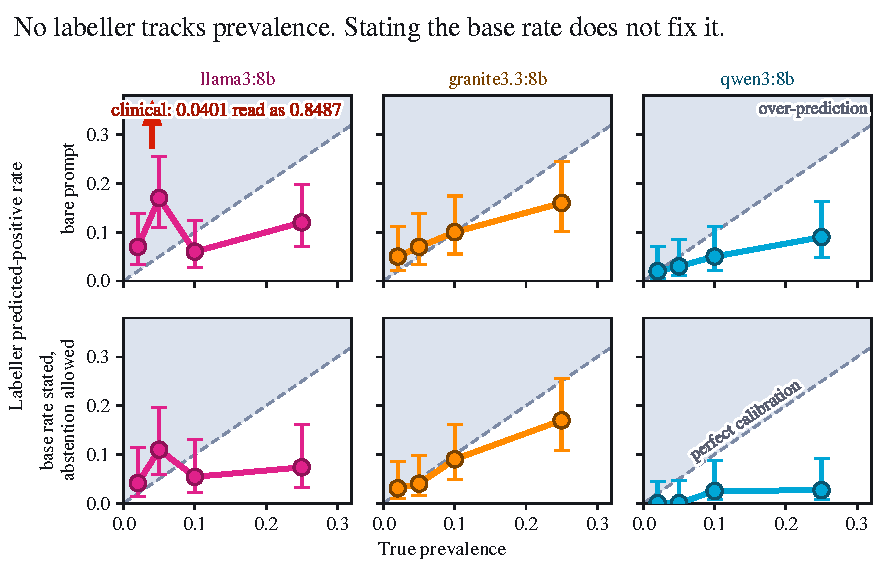
\includegraphics[width=0.98\linewidth]{figures/fig-prevalence-response.pdf}
\label{fig:prevalence-response}
\end{figure}

\subsection{The cell the design did not contain}
\label{sec:r-frontier}

Section~\ref{sec:m-control-rq2} states the condition this control was built to
decide: if over-calling is a property of one model it will not survive a change of
model, and if it is a property of the task presentation it will. The replication
changed the model three times and the domain once, and never changed the scale:
all three local labellers are eight-billion-parameter instruction-tuned models, so
the design is a two-by-two in domain and prevalence with capability held fixed, and
the cell it does not contain is a frontier-scale labeller on the clinical pool.

That cell was filled by transmitting MIMIC-III sentence pairs to hosted API
services, Claude Sonnet 5 and Claude Haiku 4.5 through the Anthropic API and
Llama 3 70B and Llama 3 8B through AWS Bedrock. PhysioNet's guidance on the use
of MIMIC data with third-party LLM services withdrew the safe-harbour list those
runs relied on (Section~\ref{sec:m-ethics}), so every one of those runs, and every
number, table, and figure computed from one, is withdrawn from this thesis. That
includes the capability ladder and the frontier discrimination table.
Whether a frontier-scale labeller removes the over-calling this chapter measures
at eight billion parameters is therefore not established here; the local-only
finding of Section~\ref{sec:res-rq2} is the one this thesis can support.

\subsection{The marginal feasibility gate}
\label{sec:r-feasgate}

Before a labeller's agreement with the pharmacist is read as evidence, its own
marginals already fix how much agreement it could possibly have shown. Holding
the confirmed count and the flagged count fixed and placing every confirmed
case inside the flagged set gives the best table those two marginals permit: a
Matthews correlation ceiling, a kappa ceiling, and the smallest one-sided
hypergeometric $p$ the labeller's own margins could return against the
pharmacist's labels. That floor $p$ is a precondition rather than a result: it
is computable before a single pair is scored, and it says whether the test
that follows could have rejected the null at all.

This bounds a thresholded decision only, and the qualification is not
optional, because the unqualified claim is false. A labeller that emits a
continuous score is not bounded this way, because the threshold that turns a
score into a flag can be swept; a model that flags most of a pool at one
threshold can still rank the pool well at another. Everything below is a
statement about labeller-and-prompt configurations in this thesis that emit a
hard label on this pool, not about a score-emitting model. One score-emitting model was measured,
under a rule registered before the run (C98): \texttt{granite3.3:8b}'s first-token
log-odds of a contradiction, graded across the $253$ non-ambiguous pairs, reaches
an AUROC of $0.5467$ (one-sided Mann-Whitney $p = 0.2934$), below the $0.7355$
this evaluation can resolve. Sweeping its threshold does not rescue it.

Table~\ref{tab:feasgate} and Figure~\ref{fig:ceiling} apply the gate to every
local labeller-and-prompt configuration this chapter scores against the
pharmacist on this pool: \texttt{granite3.3:8b} and \texttt{llama3:8b},
zero-shot and few-shot, each on both $G_{253}$ and $G_{299}$, four
configurations on two nested bases, eight rows. Two of the four,
\texttt{llama3:8b} at both prompts, could not have rejected the null at
$0.05$ on either basis before scoring a single pair, because the smallest $p$
their own marginal permits already exceeds $0.05$. Two of the four sit
exactly on their marginal-implied ceiling on both bases,
\texttt{granite3.3:8b} zero-shot and \texttt{llama3:8b} few-shot: their
observed agreement equals the best any labeller at that flag rate could
achieve, so no retuning of that labeller at that marginal could have moved it
further. The two sets overlap on \texttt{llama3:8b} few-shot, which sits on
its ceiling while unable to reject the null, the least a labeller can show at
that marginal; \texttt{granite3.3:8b} zero-shot sits on its ceiling while
rejecting the null, the most that marginal permits.

The table also carries every other hard-label marginal this chapter prints,
whether or not this project ever joined it to the pharmacist's labels row by
row: the inclusion rule is every hard-label marginal this chapter prints.
That adds five rows: the deployed weak labeller (Table~\ref{tab:marginal}),
the Llama 3 8B evaluation baseline on $G_{253}$ (Table~\ref{tab:systems253}),
and the three baseline-prompt local labellers on $G_{299}$
(Table~\ref{tab:overcalling}). The evaluation baseline is the one of these
scored row by row, and its observed MCC is printed; the other four read
\emph{not scored}. The baseline and the \texttt{llama3:8b} baseline-prompt row
are one configuration on two nested bases, so the table covers eight
configurations, not nine. Four could not have rejected the null at $0.05$ at any
outcome, all \texttt{llama3:8b}. The check was added after the hosted results
were withdrawn and is reported here as a post hoc precondition.

\begin{table}[H]
\caption[The marginal feasibility gate, every hard-label marginal this
chapter prints]{The marginal feasibility gate applied to every hard-label
labeller marginal this chapter prints: scored where this project joined the
labeller to the pharmacist row by row, unscored where only the marginal
survives.}
\centering
\footnotesize
\begin{tabular}{llrrrrrl}
\toprule
\textbf{Labeller} & \textbf{Basis} & \textbf{Flag rate} & \textbf{Obs.\ MCC} &
\textbf{Ceil.\ MCC} & \textbf{Ceil.\ $\kappa$} & \textbf{Floor $p$} & \textbf{Verdict} \\
\midrule
\texttt{granite3.3:8b}, few-shot  & $G_{253}$ & 0.6957 & 0.0668 & 0.1476 & 0.0426 & 0.0114 & Could reject \\
\texttt{granite3.3:8b}, few-shot  & $G_{299}$ & 0.7023 & 0.0586 & 0.1331 & 0.0348 & 0.0131 & Could reject \\
\texttt{granite3.3:8b}, zero-shot & $G_{253}$ & 0.7391 & 0.1326 & 0.1326 & 0.0345 & 0.0242 & Could reject, at ceiling \\
\texttt{granite3.3:8b}, zero-shot & $G_{299}$ & 0.7492 & 0.1183 & 0.1183 & 0.0276 & 0.0290 & Could reject, at ceiling \\
\texttt{llama3:8b}, few-shot      & $G_{253}$ & 0.9447 & 0.0540 & 0.0540 & 0.0058 & 0.4971 & Could not reject, at ceiling \\
\texttt{llama3:8b}, few-shot      & $G_{299}$ & 0.9398 & 0.0518 & 0.0518 & 0.0053 & 0.4679 & Could not reject, at ceiling \\
\texttt{llama3:8b}, zero-shot     & $G_{253}$ & 0.8735 & 0.0290 & 0.0849 & 0.0143 & 0.1898 & Could not reject \\
\texttt{llama3:8b}, zero-shot     & $G_{299}$ & 0.8729 & 0.0269 & 0.0780 & 0.0121 & 0.1894 & Could not reject \\
\midrule
Llama 3, deployed weak labeller       & $G_{299}$ & 0.8729 & not scored & 0.0780 & 0.0121 & 0.1894 & Could not reject \\
Llama 3 8B eval.\ baseline, prompted once & $G_{253}$ & 0.9565 & $-0.0436$ & 0.0476 & 0.0045 & 0.5795 & Could not reject \\
\texttt{llama3:8b}, baseline prompt      & $G_{299}$ & 0.9532 & not scored & 0.0453 & 0.0041 & 0.5562 & Could not reject \\
\texttt{granite3.3:8b}, baseline prompt  & $G_{299}$ & 0.7425 & not scored & 0.1204 & 0.0286 & 0.0259 & Could reject \\
\texttt{qwen3:8b}, baseline prompt       & $G_{299}$ & 0.6187 & not scored & 0.1605 & 0.0502 & 0.0027 & Could reject \\
\bottomrule
\end{tabular}
\apanote{Ceiling MCC and ceiling $\kappa$ hold every confirmed case inside the
flagged set. Of the five rows below the rule only the evaluation baseline was
scored row by row; the others read \emph{not scored}. Floor $p$ is the smallest one-sided hypergeometric $p$ the marginal
allows (Section~\ref{sec:r-multiplicity}), a precondition rather than a test
unless observed MCC equals ceiling MCC, where it is also the exact test
observed. Basis is $G_{253}$ or $G_{299}$ (Table~\ref{tab:denoms}); every
cell is generated, none is typed.}
\label{tab:feasgate}
\end{table}

\begin{figure}[t]
\centering
\caption[The agreement ceiling a labeller's marginal imposes]{Largest Cohen's
kappa any thresholded labeller can reach against the pharmacist, as a function of
its positive rate on the $299$ gold pairs. The curve is an identity of the two
marginals, not a fit, so it carries no interval. Marked rows attain their own
ceiling. A labeller emitting a score is not bounded this way, because its
threshold can be swept.}
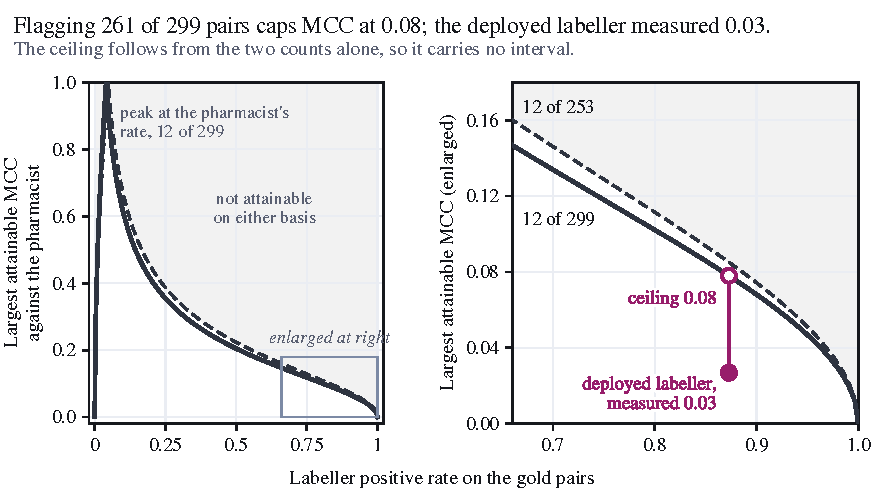
\includegraphics[width=0.98\linewidth]{figures/fig-ceiling.pdf}
\label{fig:ceiling}
\end{figure}

What the gate does not do is replace the discrimination tests reported
elsewhere in this chapter; it is read beside them, as a check on what a table
could have shown before it is read as showing it. A labeller whose floor sits
above the threshold, \texttt{llama3:8b} at both prompts here, was never going
to distinguish itself from chance at this marginal, and a labeller sitting on
its ceiling flagged every confirmed positive; at that flag rate it could not
have scored higher, whatever it otherwise knew about the pairs.

\subsection{What the false positives land on}
\label{sec:r-ambiguity}

Whether a labeller concentrates its false positives on the pairs the
pharmacist declined to call, rather than spreading them evenly across the
$287$ non-confirmed pairs, was tested by a one-sided Fisher exact test on flag
rate, ambiguous against clear-negative, replicated across labellers under two
prompts each. Four hosted labellers under two prompts each were tested this
way, eight tests in total; every one was run through the Anthropic API or AWS
Bedrock, so every odds ratio, every $p$ value, and the gradient itself are
withdrawn with the runs that produced them (Section~\ref{sec:r-frontier}). The
two local labellers were put to the same test: \texttt{granite3.3:8b} returns
an odds ratio of $1.2801$ at $p = 0.3110$ few-shot and $1.5505$ at $p = 0.1788$
zero-shot; \texttt{llama3:8b} returns $0.6476$ at $p = 0.8577$ few-shot and
$0.9841$ at $p = 0.6220$ zero-shot, none rejecting the null at $0.05$
(Section~\ref{sec:r-multiplicity}). This chapter therefore does not establish
that the ambiguous pairs are disproportionately flagged by any labeller
tested. The one confound that would have bounded any surviving reading, that an
odds ratio compresses toward $1$ as a labeller's marginal saturates, applies
to the local tests just reported as much as to the withdrawn ones.

\subsection{What the instability costs, and what it does not}
\label{sec:r-labelnoise}

A label-instability analysis was run on the frontier labeller's per-pair
draws, asking how much a Matthews correlation would move if individual labels
flipped at random. Every cell that analysis read from is a hosted-API result
and is withdrawn along with it (Section~\ref{sec:r-frontier}); no equivalent
instability bound is reported for a local labeller in this thesis, because the
open-weights runs were single deterministic draws under greedy decoding rather
than a resampled distribution over labels.

\section{Architecture}
\label{sec:res-rq3}

Do the purpose-built components contribute what they were credited with? No
component survives what a code audit finds. No randomisation control was run
on any of these three clinical components; what follows are audit findings,
not controls firing: one parameter is falsified as an initialisation artifact,
one metric is vacated by label leakage, and one module was never trained.

\subsection{One falsified, one vacated by leakage, one never trained}

\paragraph{Authority conditioning is an initialisation artifact.} The parameter
reported as converging to the clinical note hierarchy is initialised at $1.0$
for the discharge branch and $0.5$ for the nursing branch, the exact pair
reported as discovered by training. Across three seeds the discharge value
ends between $1.0024$ and $1.0047$, mean $1.0038$, and the nursing value ends
between $0.5070$ and $0.5084$, mean $0.5076$. Both parameters move a small
fraction of their initial value across seeds. Each sits on a branch that is
immediately normalised, which removes most of what a per-branch scalar can do
and drives its gradient towards zero.

\paragraph{The rule-type head is label leakage.} The rule identifier is written
into the model's input feature vector and predicted from the same forward pass,
one linear layer away, so the auxiliary task is a copy. Out-of-domain transfer is
the diagnostic that separates a copy from learned structure, because the leaked
feature survives transfer and the surface correlations do not. This belongs to
the documented family of shortcut learning \citep{geirhos2020shortcut,
zech2018generalization}; the checkable point is narrower, that an auxiliary head
whose target is derivable from its inputs is not an auxiliary task. In domain the
rule-type head reaches a macro $F_1$ of $0.9603$. Transferred without retraining
it collapses by more than an order of magnitude on both secondary cohorts, as
Table~\ref{tab:transfer} records. That is
reported as a descriptive non-portability
result rather than further evidence of leakage: the code-level argument above
is dispositive on its own, and a literal copy of the rule-identifier feature
would transfer perfectly, since the feature and target stay
identical in any domain. The collapse instead shows that the in-domain macro
$F_1$ reflects the correlation between that feature and this cohort's label
distribution rather than a verbatim copy of it, a correlation that does not
hold in the transfer cohorts.

\begin{table}[H]
\centering
\caption[Rule-type head under cohort transfer]{The rule-type head in domain and
transferred without retraining. No interval is committed for any of these three
values, so none is printed and none should be inferred; they are single
measurements on the candidate counts shown.}
\label{tab:transfer}
\begin{tabular}{lrr}
\toprule
\textbf{Cohort} & \textbf{Candidates} & \textbf{Macro $F_1$} \\
\midrule
Heart failure, training domain & 1,978 & 0.9603 \\
Sepsis                         &   775 & 0.0654 \\
Acute kidney injury            & 1,983 & 0.0595 \\
\bottomrule
\end{tabular}
\end{table}

\paragraph{Harm estimation was never trained.} The guideline bank is one randomly
initialised parameter matrix, there is no corpus and no retrieval step, and the
harm head does not appear in the training objective. Over the 299 annotated
pairs its output ranges from $0.3977$ to $0.6096$, a narrow band
consistent with an untrained scorer rather than a calibrated severity measure.
Its rank correlation against the pharmacist danger rating over all 299 pairs is
$\rho = -0.0001$, $p = 0.9991$. The
severity-ranking question was therefore not tested, and any null reported
against that head measures an untrained module rather than the underlying
question.

\subsection{Three controls that fired positively}

These controls run on a second system: a provenance-conditioned encoder trained with masked
language modelling, not the clinical contradiction detector whose numbers appear elsewhere in this
chapter.

\paragraph{A control task, a thesis-original alignment control, and locality alone.} Ten arms of a
shared additive attention bias were trained on masked language modelling over packed multi-document
bundles with segment order shuffled so role is decorrelated from position
(Section~\ref{sec:m-control-rq3}). Seven ran at three seeds each and are the matched comparison the
condition specifies; three ran at a single seed each, reported for completeness, not as
matched comparisons against the three-seed rows. Table~\ref{tab:ablation} reports the mean
validation loss, its seed spread where more than one seed exists, and the loss reduction against the
no-bias arm for all ten.

\begin{table}[H]
\caption[Ten-arm architecture ablation results]{Ten-arm architecture ablation, mean validation loss.}
\label{tab:ablation}
\centering
\small
\begin{tabular}{lrrrrr}
\toprule
\textbf{Arm} & \textbf{Mean val.\ loss} & \textbf{SD} & \shortstack[r]{\textbf{$\Delta$ vs.}\\\textbf{vanilla}} &
\shortstack[r]{\textbf{\% of segment-}\\\textbf{index gain}} & \textbf{Seeds} \\
\midrule
Global positions restored  & 4.5122 & n/a & +0.1567 & n/a     & 1 \\
Vanilla, no bias           & 4.3554 & 0.0085 & 0       & 0\%     & 3 \\
T5 relative position bias  & 4.1035 & 0.0029 & -0.2520 & 26.6\%  & 3 \\
Length-bucket roles        & 4.0174 & n/a & -0.3380 & 35.7\%  & 1 \\
Misaligned block bias      & 3.9109 & 0.0293 & -0.4445 & 46.9\%  & 3 \\
Random roles (shuffled)    & 3.8587 & n/a & -0.4967 & 52.4\%  & 1 \\
ALiBi distance bias        & 3.7435 & 0.0023 & -0.6119 & 64.6\%  & 3 \\
True role labels           & 3.5310 & 0.0076 & -0.8244 & 87.0\%  & 3 \\
Segment-index bias         & 3.4078 & 0.0225 & -0.9476 & 100\%   & 3 \\
Hard block mask, fixed     & 3.2772 & 0.0124 & -1.0782 & 113.8\% & 3 \\
\bottomrule
\end{tabular}
\apanote{Mean validation loss and its SD are given per arm, with the change against vanilla and its share of the segment-index arm's reduction, the largest gain among the three-seed arms; the share is undefined for the global-positions row, which increases loss relative to vanilla. Seed spreads on the seven three-seed rows run from $0.0023$ to $0.0293$ nats against effects from $0.2520$ to $1.0782$ nats, so every ordering among them is resolved well outside seed noise. The three single-seed rows carry no spread and are shown for completeness only.}
\end{table}

Two rows in Table~\ref{tab:ablation} are stated as a finding, not as a
control check run on the way to one. A hard block mask with zero trainable
parameters, fixed rather than learned, beats every learned attention-bias arm
in the table, including the segment-index bias it was built to bound. And an
arbitrary positional ordinal carrying no provenance meaning beats true
role labels. Neither result bears on the clinical contradiction detector or
its precision reported elsewhere in this chapter.

The control task in the
sense \citet{hewitt2019control} define it is the random-roles arm, which holds
the label alphabet fixed and randomises the mapping from tokens to roles; it
ran at a single seed, so no significance claim attaches to it, and true role
labels reduce the loss more than that randomisation does, a directional gap
consistent with role semantics contributing something real on this seed. A
second single-seed arm, roles collapsed to length buckets, points the same
direction. The segment-index arm is different in kind: it substitutes an
arbitrary ordinal position for role identity rather than randomising role
identity, so a win for it is a competing hypothesis about what the mechanism
exploits, not a control task in the \citet{hewitt2019control} sense and not
evidence that role semantics contribute nothing. It is the largest
reduction of any learned arm, ahead of true role labels, so the two results
point the same direction rather than opposite ones.

The misaligned-block arm, this thesis's own addition to that design, holds the
block count fixed at the aligned segment-index arm's count and destroys only
the alignment with the note boundaries the arm was built to mark. It recovers
under half of the aligned arm's reduction, closing the alternative reading
that any coarse partition of the attention matrix would do as well. The ALiBi
arm carries no segment information, only a monotonic penalty on
token distance, and still recovers close to two thirds of the segment-index
arm's reduction: locality alone, with no representation of which document a
token belongs to, accounts for most of the effect credited to
provenance-aware conditioning. The fixed hard block mask, the encoder analogue
of the intra-document mask \citet{zhao2024seqcomposition} apply during causal
decoder pretraining (adapted here to masked language modelling), learns
nothing and only blocks attention across the announced document boundary, yet
beats every learned arm.

One single-seed arm checks a standing confound directly: every other arm
trains without global position information, so the segmentation gain could
be a positionally handicapped baseline buying position back rather
than a genuine effect of provenance conditioning. Restoring global positions
on top of the shuffled-segment setup recovers none of the segment-index gain:
the confound this control was built to rule out does not hold.

\paragraph{The anisotropy control.} The third control targets the proposed
explanation rather than the effect: if the behaviour follows from
representational anisotropy in the encoder, removing the anisotropy removes the
behaviour. The control condition's mean pairwise similarity is
$0.9113$ and the matched clinical-pair mean is $0.9176$, a difference of
$0.0063$. A Welch two-sample $t$-test on
the two conditions' registered means, standard deviations and counts gives
$t = 4.0001$ on $235.84$ degrees of freedom,
which rejects exact equality at conventional significance thresholds; with
$190$ pairs in the control condition and $1{,}956$ in the clinical one, a
difference this small is still detectable, and $t$ alone reflects that
sample size as much as the size of the difference.

That degrees-of-freedom figure is not defensible: the $190$ control
observations are every pairwise similarity among $20$ sentences, $190$ being
exactly $20$ choose $2$, so each sentence enters nineteen of them, the
observations are not independent draws, and the number of independent units
is closer to $20$ than to $190$. The standard error, and the $p$ value with
it, is understated by a factor this thesis does not compute, and the two
samples are also built differently, all pairwise combinations against
$1{,}956$ matched pairs, so this is not a like-for-like unpaired comparison
either. What survives is the effect size, the pooled-standard-deviation
Cohen's $d$ of $0.2808$, a small effect by conventional benchmarks that does
not depend on the degrees of freedom; nothing rests on the $p$ value,
which Section~\ref{sec:r-multiplicity} reads at the single uncorrected
threshold this chapter applies throughout, not as a result that has cleared
anything. Equality is therefore not claimed.
What is claimed is that the difference is small against the spread the same
extraction path produces on unrelated text, which ranges from $0.8528$ to
$0.9565$: unrelated non-clinical sentence pairs
land within a few hundredths of matched clinical pairs, close enough that the
proposed mechanism, present and manipulated, does not carry the outcome it was
credited with.

No arm in this table carries a significance claim; no test was run on any of
the ten. What it establishes divides by seed count instead: the seven
three-seed arms are resolved well outside seed noise, while the random-roles
control task and the segment ordinal ran at a single seed each and are read as
direction only.

\section{Is the Null Real}
\label{sec:res-rq4}

Every negative result above reduces to ``the experiment was too small'' unless
the instrument can be shown to resolve an effect of the size at issue. Three
configurations of the detector sit at chance, a paired comparison cannot separate
two of them, a bag-of-words baseline outranks all of them, and the minimum
detectable effect is large. Then a positive control, adjudicated by a rule
committed before the sweep ran, shows the same apparatus resolving a real effect.

\subsection{Three configurations at chance}

\begin{table}[H]
\caption[Decontaminated detector at chance]{Decontaminated detector on the 253 non-ambiguous pairs.}
\centering
\small
\begin{tabular}{lrrrr}
\toprule
\textbf{Configuration} & \textbf{AUROC} & \textbf{AP} &
\textbf{Mann-Whitney $p$} & \textbf{Top-15 TP} \\
\midrule
Seed 0              & 0.5494 & 0.0613 & 0.5646 & 1 \\
Seed 1              & 0.5090 & 0.0592 & 0.9179 & 0 \\
Seed 2              & 0.5048 & 0.0533 & 0.9565 & 0 \\
Per-seed mean (SD)  & 0.5211 (0.0201) & & & \\
Three-seed ensemble & 0.5145 & & 0.8668 & \\
\midrule
Contaminated run, same 253 pairs & 0.4595 & & 0.6418 & \\
\bottomrule
\end{tabular}
\apanote{$G_{253}$, 12 positives and 241 negatives; bootstrap resampling uses $B = 10{,}000$ at seed 42. Average precision is the appropriate summary at this imbalance \citep{saito2015prcurve} and its no-skill line is $12/253$. The percentile bootstrap interval for the ensemble AUROC on $G_{253}$ is $0.3210$ to $0.7034$. The per-seed standard deviation is computed at $\mathrm{ddof} = 0$, the population convention (Section~\ref{sec:m-stats}), and is not compared against a spread computed under the sample convention.}
\label{tab:decontam}
\end{table}

\begin{table}[H]
\caption[Operating point of the decontaminated detector]{The decontaminated
detector at its decision threshold, per seed and as a mean, on the $253$
non-ambiguous pairs.}
\centering
\small
\begin{tabular}{lrrrrrrrr}
\toprule
\textbf{Seed} & \textbf{TP} & \textbf{FP} & \textbf{FN} & \textbf{TN} &
\textbf{Precision} & \textbf{Recall} & \textbf{$\kappa$} & \textbf{ECE} \\
\midrule
0            & 9  & 216 & 3 & 25 & 0.0400 & 0.7500 & $-0.0155$ & 0.8321 \\
1            & 10 & 210 & 2 & 31 & 0.0455 & 0.8333 & $-0.0041$ & 0.7942 \\
2            & 9  & 207 & 3 & 34 & 0.0417 & 0.7500 & $-0.0120$ & 0.7782 \\
\midrule
Mean         &    &     &   &    & 0.0424 & 0.7778 & $-0.0105$ & 0.8015 \\
SD           &    &     &   &    & 0.0023 & 0.0393 & 0.0048 & 0.0226 \\
\bottomrule
\end{tabular}
\apanote{Threshold $0.5$; each row sums to $253$. Precision at $0.0424$ sits within one binomial standard error, $0.0134$, of the confirmed rate $0.0474$. Recall is high because the detector is near-degenerate, returning positive for $207$ to $216$ of the $241$ clear negatives; expected calibration error above $0.78$ and $\kappa$ below zero in every seed reflect that. Standard deviations use $\mathrm{ddof} = 0$ (Section~\ref{sec:m-stats}); Table~\ref{tab:control299} uses the sample convention and is not compared here.}
\label{tab:operating}
\end{table}

The ensemble's 95 percent bootstrap interval (Table~\ref{tab:decontam}) is wide
enough at 12 positives to sit on both sides of chance, so the positive and
negative score distributions are not separated. The contaminated run, trained
on the pairs it scores, lands below chance on the same 253 pairs: leakage did
not manufacture signal, because there was none to manufacture.

\begin{table}[H]
\caption[Control model and contaminated run, full set and stratum]{The defect-free control model
and ACCORD's contaminated released run, scored on the same pairs.}
\centering
\small
\begin{tabular}{llrrrr}
\toprule
\textbf{Set} & \textbf{Configuration} & \textbf{AUROC} & \textbf{AP} &
\textbf{Boot.\ mean} & \textbf{Boot.\ SD} \\
\midrule
$G_{299}$ & Control model, three-seed ensemble & 0.4692 & 0.0512 & 0.4699 & 0.0937 \\
$G_{299}$ & Control model, per-seed mean $\pm$ SD & \multicolumn{4}{l}{$0.4967 \pm 0.0350$ (AP $0.0491 \pm 0.0024$)} \\
$G_{299}$ & ACCORD, contaminated released run & 0.4602 & 0.0394 & 0.4606 & 0.0870 \\
\midrule
$G_{134}$ & Control model, three-seed ensemble & 0.5469 & 0.0784 & 0.5479 & 0.1481 \\
$G_{134}$ & Control model, per-seed mean $\pm$ SD & \multicolumn{4}{l}{$0.5295 \pm 0.0158$ (AP $0.0707 \pm 0.0108$)} \\
$G_{134}$ & ACCORD, contaminated released run & 0.5078 & 0.0555 & 0.5092 & 0.1368 \\
\bottomrule
\end{tabular}
\apanote{Bootstrap columns are the mean and SD over $B = 10{,}000$ resamples at seed $20{,}260{,}806$ \citep{efron1994bootstrap}. The four control-model rows are the defect-free control model of Section~\ref{sec:m-control-model}, three seeds, subject-disjoint split. The two ACCORD rows are the contaminated released run of Tables~\ref{tab:rule-precision}, \ref{tab:marginal} and \ref{tab:systems253}; its $G_{253}$ counterpart is the $0.4595$ in Table~\ref{tab:decontam}. It is the only ACCORD score on $G_{134}$, and Table~\ref{tab:delong}'s DeLong tests compare against it. Per-seed SD uses $\mathrm{ddof} = 1$ (Section~\ref{sec:m-stats}), unlike Table~\ref{tab:decontam}'s $\mathrm{ddof} = 0$; the two are not compared.}
\label{tab:control299}
\end{table}

The three configurations agree. The contaminated released run, the
decontaminated ensemble, and the stratum free of the exemplar defect all
return a ranking statistic within a few points of chance. Restricting to
$G_{134}$ (Table~\ref{tab:control299}) raises the ensemble's point estimate
and its bootstrap spread, so halving the positive count buys a higher
estimate and a wider spread, and resolves nothing either way.

Among the fifteen highest-scored pairs, the decontaminated seeds recover 1, 0 and
0 true contradictions on $G_{253}$; on $G_{299}$ the three control seeds
recover 1, 0 and 0, their ensemble recovers 1, and the contaminated released run,
which the note to Table~\ref{tab:control299} is explicit is not a control
configuration, recovers 0, against expected counts of
$15 \times 12/253$ and $15 \times 12/299$ under random ordering. A count of one
is unremarkable, and that is the point: the model's most confident predictions
are indistinguishable from a random draw. For a ranked worklist that is decisive.

One objection to Table~\ref{tab:operating} has to be answered rather than left standing: the
table reports the configured threshold of $0.5$, and a threshold is a free parameter, so a
different cutoff might expose signal the table hides. The answer is the best Matthews
correlation attainable at any cutoff whatever, chosen with the pharmacist's labels already in
hand. On $G_{253}$ it is $0.0554$ on the contradiction probability and $0.0631$ on the harm
score.

Those two figures must not be read against zero: a statistic maximised over a
tuning parameter on the same sample it is evaluated on is not centred at zero
under the null, since the maximum of a noisy process is positive by
construction. Against the same maximisation run on random scores at this
sample size and positive count, whose median is $0.0968$, the observed
optima sit at the $0.8195$ and $0.7642$ points, so the best cutoff that
exists performs worse than roughly four in five pure-noise runs: no threshold
rescues this detector, and the operating point in Table~\ref{tab:operating}
is not an unlucky choice of one. The harm-score optimum rests on two true
positives and is quoted only as a bound.

These figures come from the released score file, the contaminated release,
not from the three-seed run behind Table~\ref{tab:operating}, and a reader
recomputing the operating point from the released file will get a different
number. Within the released file the harm score at $0.5$ is a
near-constant positive like the table, so the direction is not even
consistent across decision variables within one file. Both are degenerate,
neither discriminates, and no claim here turns on which.

\subsection{The paired comparison}

\begin{table}[H]
\caption[Paired ROC comparisons by DeLong test]{Paired ROC comparisons of the control model against ACCORD's contaminated released run, on the same pairs.}
\centering
\small
\begin{tabular}{llrrrrr}
\toprule
\textbf{Set} & \textbf{Comparison} & \textbf{AUC A} & \textbf{AUC B} &
\textbf{Diff.} & \textbf{$z$} & \textbf{$p$} \\
\midrule
$G_{299}$ & Control ensemble vs.\ ACCORD  & 0.4692 & 0.4602 & $0.0090$  & $0.0878$  & 0.9300 \\
$G_{299}$ & Control seed 42 vs.\ ACCORD   & 0.4591 & 0.4602 & $-0.0012$ & $-0.0110$ & 0.9912 \\
$G_{299}$ & Control seed 123 vs.\ ACCORD  & 0.5029 & 0.4602 & $0.0427$  & $0.4358$  & 0.6630 \\
$G_{299}$ & Control seed 2024 vs.\ ACCORD & 0.5282 & 0.4602 & $0.0679$  & $0.7028$  & 0.4822 \\
$G_{134}$ & Control ensemble vs.\ ACCORD  & 0.5469 & 0.5078 & $0.0391$  & $0.7881$  & 0.4306 \\
\bottomrule
\end{tabular}
\apanote{DeLong's test for two correlated ROC curves \citep{delong1988comparing}. Standard errors of the difference are $0.1025$, $0.1052$, $0.0979$, $0.0967$ and $0.0496$ for the five rows in order. The AUC B column is ACCORD's contaminated released run throughout; these are five comparisons of the control model against that one run, not comparisons among control configurations.}
\label{tab:delong}
\end{table}

The seeds and the ensemble are correlated predictors scored on the same pairs,
so the comparison has to be paired, and the first row carries the section: its
standard error on the difference is eleven times the difference itself. Every
row has that shape, and at 12 positives none could have another.

\subsection{A bag-of-words baseline}

Table~\ref{tab:baselines} carries the comparison.

\begin{table}[H]
\caption[Reference baselines on annotated pairs]{Reference baselines on the annotated pairs.}
\centering
\small
\begin{tabular}{llrrr}
\toprule
\textbf{Set} & \textbf{Baseline} & \textbf{AUROC} & \textbf{AP} &
\textbf{Top-15 TP} \\
\midrule
$G_{299}$ & TF-IDF plus logistic regression & 0.5761 & 0.1571 & 2 \\
$G_{299}$ & Majority class                  & 0.5000 & 0.0401 & n/a \\
$G_{134}$ & TF-IDF plus logistic regression & 0.5729 & 0.2768 & 2 \\
$G_{134}$ & Majority class                  & 0.5000 & 0.0448 & n/a \\
\bottomrule
\end{tabular}
\apanote{Both baselines are fitted on 1,183 training rows at a positive rate of $0.8521$, the same weak supervision the detector consumed; TF-IDF is capped at 5,000 features. A majority-class predictor assigns every row the identical score, so it has no ranking among rows and no well-defined top 15; the column is marked n/a for both majority-class rows rather than reporting whatever count an arbitrary tie-break happened to produce. The majority-class average precisions are the base rates of the two sets and fix the no-skill line for that column.}
\label{tab:baselines}
\end{table}

TF-IDF plus logistic regression outperforms every $G_{299}$ and $G_{134}$
neural configuration in Table~\ref{tab:control299}, the matched sets it was
evaluated on; it was not run on $G_{253}$, so no comparison is drawn here
against Table~\ref{tab:decontam}. It puts two true contradictions in its top
fifteen on both sets. No significance is claimed for that ordering. It does
establish that a
domain-pretrained encoder \citep{gu2021biomedbert} with low-rank adaptation
\citep{hu2022lora} does not clear a linear model over 5,000 n-gram counts.

\subsection{What the instrument could have seen}

\begin{table}[H]
\caption[Minimum detectable AUROC by evaluation size]{Minimum detectable AUROC at 80\% power.}
\centering
\small
\begin{tabular}{lrrrrr}
\toprule
\textbf{Set} & \textbf{Positives} & \textbf{Negatives} &
\textbf{SE under null} & \textbf{Gap} & \textbf{Min.\ detectable} \\
\midrule
$G_{253}$ & 12 & 241 & 0.0856 & 0.2355 & 0.7355 \\
$G_{299}$ & 12 & 287 & 0.0852 & 0.2350 & 0.7350 \\
$G_{134}$ & 6  & 128 & 0.1210 & 0.3058 & 0.8058 \\
\bottomrule
\end{tabular}
\apanote{$\alpha = 0.05$, power $0.8$. The SE column is the simple null-standard-error approximation. The Gap and Min.\ detectable columns follow the full \citet{hanley1982meaning} procedure (superseded value: R9). The gap column is the distance above chance the evaluation could resolve.}
\label{tab:power}
\end{table}

On $G_{253}$ nothing below an AUROC of $0.7355$ was detectable at $80\%$ power,
and the measured $0.5145$ is far inside that. Figure~\ref{fig:power} draws the
same ceiling for every evaluation in this thesis. This cuts both ways: at 12
positives the evaluation could not have detected
a useful detector unless it was very good, so the null does not establish that
the task is unsolvable. What it does establish is that this pipeline produced
nothing near the detectable range, and it fixes the size of the annotation effort
a future attempt needs.

\begin{figure}[!ht]

\centering
\caption[Minimum detectable effect by evaluation size]{Minimum detectable AUROC
at 80\% power and two-sided $\alpha$ of 0.05, by Hanley and McNeil
\citep{hanley1982meaning}, against the number of positives in the evaluation
set. The circle is this thesis's contradiction evaluation; the square is the
mortality positive control.}
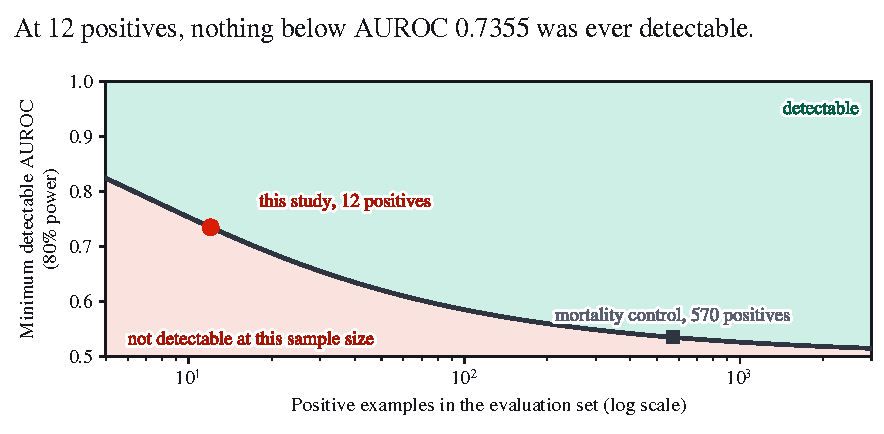
\includegraphics[width=0.98\linewidth]{figures/fig-power.pdf}
\label{fig:power}
\end{figure}

The minimum detectable AUROC comes from a formula this thesis has
already found unreproducible once (Appendix~\ref{app:corrections}, R9). A
Monte Carlo check, written for this thesis and released with it, draws
$5{,}000$ synthetic score sets at this evaluation's class counts ($12$
positives, $241$ negatives) from an equal-variance binormal calibrated to
each target AUROC and records how often a two-sided Mann-Whitney test at
$\alpha = 0.05$ rejects; its interpolated crossing of $80\%$ power, $0.7324$,
agrees with the analytic $0.7355$ to within three thousandths of an AUROC
point. Because its only inputs are the class counts, $\alpha$, and the target
grid, with no ACCORD score, gold label, or clinical data, this is a numerical
corroboration that $0.7355$ was computed correctly, not an empirical check on
the instrument. The claim that survives is the one the formula already
supported: the $253$-pair evaluation's null is informative about true AUROC
values at or above $0.7355$ and silent below that line.

\subsection{Multiplicity, and what is not corrected for}
\label{sec:r-multiplicity}

\textbf{No multiple-comparison correction is applied anywhere in this thesis.}
The single threshold every reported $p$ value in this chapter is read against
is the conventional $\alpha = 0.05$, uncorrected, and no result in this
chapter is described as surviving or clearing a correction it was never
subjected to. Sidedness is stated plainly rather than left implicit: the
Mann-Whitney tests of Table~\ref{tab:decontam}, the DeLong tests of
Table~\ref{tab:delong}, the mechanism Fisher test, the Welch test on the
anisotropy control, and the minimum-detectable-effect calculation of
Section~\ref{sec:res-rq4} are all two-sided; the local ambiguity-gradient
Fisher tests and the feasibility gate's attainable floor are one-sided,
because each bounds the most agreeable outcome a marginal permits; sidedness
for the Spearman correlations below is not recorded in the artifact behind
them. The gate's hypergeometric floors (Table~\ref{tab:feasgate}) are
preconditions, not members of this family: each is computable before a pair
is scored, so it bounds what a test could show rather than testing what was
observed. A correction record documents this history (C68, C76, C79, C85,
C88, C90, C92) rather than narrating it.

The tests this chapter still reports are enumerated in the committed register
released with the analysis code, one entry per test bound to the artifact and
key its $p$ value is read from; the withdrawal removed the eight frontier
Fisher exact tests, the four frontier Mann-Whitney tests, the four Bedrock
discrimination tests, and the eight hosted ambiguity-gradient tests, because
the runs behind every one of them are withdrawn (Section~\ref{sec:r-frontier}).
What remains is the five Mann-Whitney tests of Table~\ref{tab:decontam}, the
five DeLong tests of Table~\ref{tab:delong}, the one Fisher exact test on the
Rule 1/2 versus Rule 3/4 mechanism split (Section~\ref{sec:res-rq1}), the four
local Fisher exact tests on the ambiguity gradient
(Section~\ref{sec:r-ambiguity}), the one Welch two-sample $t$ test on the
anisotropy control, and four Spearman rank correlations against the
pharmacist's danger rating. No committed script has recomputed a family size
since the withdrawal, so none is typed here: the current count is in the
register.

A test belongs to this family by its inferential target, not by what a run
was commissioned for: two tests asking the same question of the same rows
count once regardless of which experiment produced the artifact, a
sensitivity analysis on a nested subset is a robustness check rather than a
second test, and a test whose target is this project's own bookkeeping, such
as the joinability check of Section~\ref{sec:r-exemplar}, is outside every
family (C90). No surviving block is close to independent: the five
Mann-Whitney tests are three seeds of one model, their ensemble, and one
further run, all on the same $253$ rows; the five DeLong tests are five
comparisons against a single reference run; and the four local ambiguity
tests are two models under two prompts each, scored on the same $46$
ambiguous and $241$ clear-negative pairs. The absence of a rejection across
any correlated block is weaker evidence than the same absence would be for a
single pre-specified test, and any single rejection inside one would be
correspondingly weaker evidence.

Two more Spearman tests against the same target are disclosed here rather
than left out silently: the contradiction-probability score against the
danger rating returns $\rho = -0.0286$ at $p = 0.6224$ over all $299$ pairs
and $\rho = -0.2771$ at $p = 0.3833$ over the $12$ positives, and the harm
score against the rating restricted to the $12$ positives returns
$\rho = -0.6621$ at $p = 0.019$, nominally below $0.05$ on twelve cases;
Section~\ref{sec:res-rq3} already reports the fourth, the harm score over all
$299$ pairs. None of the four is treated as evidence of anything, since the
harm head is already read as untrained and the contradiction-probability
score is this project's own detector rather than an external labeller;
reporting only the null members of a family the reader cannot see is the
defect this subsection exists to prevent.

\subsection{The positive control}

The remaining objection is that the apparatus, the training loop, the
splits, the seeds and the evaluation harness, cannot resolve any effect, and that
is answerable only by running the same apparatus where an effect is known to
exist. The control has a public arm, AG News, and a clinical arm built for
this control rather than for its own sake, in-hospital mortality predicted
from a patient's first 48 hours of notes, evaluated on $6{,}776$ held-out
admissions holding $570$ positives, a different task and cohort from
the $253$-pair contradiction evaluation. Four arms on the public task,
a pretrained encoder and three from-scratch encoders at different
pretraining scales, were each trained at 3, 6, 12 and 24 epochs, three seeds
per cell, for 48 runs and 555 minutes of compute. The adjudication rule
(Table~\ref{tab:m-prereg}) was committed before the sweep ran: a gap of at
least $3.0$ accuracy points between the pretrained arm and the best
from-scratch arm at the longest budget, with non-overlapping
one-standard-deviation bands, licenses reading the clinical null as measured;
a smaller or unresolved gap reverts it to an insensitivity finding; $2.5$ to
$3.5$ points is inconclusive in advance, and the rule forbids resolving that
by adding seeds.

\begin{table}[H]
\caption[Convergence sweep across training budgets]{Convergence sweep: four arms at four training budgets.}
\centering
\small
\begin{tabular}{lrrrr}
\toprule
\textbf{Arm} & \textbf{3 epochs} & \textbf{6 epochs} & \textbf{12 epochs} &
\textbf{24 epochs} \\
\midrule
Pretrained encoder & 0.9392 (0.0012) & 0.9369 (0.0004) & 0.9375 (0.0012) & 0.9379 (0.0029) \\
Scratch, 100M      & 0.8885 (0.0012) & 0.8903 (0.0034) & 0.8888 (0.0011) & 0.8925 (0.0004) \\
Scratch, 30M       & 0.8833 (0.0009) & 0.8856 (0.0035) & 0.8845 (0.0022) & 0.8886 (0.0015) \\
Scratch, 10M       & 0.8784 (0.0022) & 0.8795 (0.0013) & 0.8822 (0.0011) & 0.8838 (0.0036) \\
\bottomrule
\end{tabular}
\apanote{Accuracy, three seeds per cell, SD in parentheses; 48 runs, 555 minutes total, topic classification on AG News. The adjudication rule, committed at commit \texttt{b048829} before the sweep ran: Outcome A is a gap of at least $3.0$ points with disjoint SD bands; Outcome B is a gap below $3.0$ or an unresolved ordering; $2.5$ to $3.5$ is inconclusive in advance, and the rule forbids resolving that by adding seeds. Prose gaps use unrounded values, not these four-decimal cells, which can differ in the last digit.}
\label{tab:conv}
\end{table}

The gap between the pretrained arm and the best from-scratch arm is $5.07$ points
at 3 epochs and $4.53$ points at 24. Eight times the budget moved the pretrained
arm by $-0.13$ points and the 100M from-scratch arm by $0.41$. The gap did not
close, the arms had converged by the smallest budget in the sweep, and every cell
has a seed-to-seed standard deviation at or below $0.0036$. That is the harness
resolving a real effect on the public task; on the mortality control task the
same harness returns a gap of $0.0031$, reported next.

\begin{table}[H]
\caption[Pretraining gap versus parameter count]{Pretraining against parameter count, and the same contrast on the
mortality control task.}
\centering
\small
\begin{tabular}{llrr}
\toprule
\textbf{Task} & \textbf{Arm} & \textbf{Parameters} & \textbf{Score} \\
\midrule
Public benchmark  & Pretrained encoder & 85,648,132 & $0.9396 \pm 0.0010$ \\
Public benchmark  & Scratch, 100M      & 99,234,820 & $0.8878 \pm 0.0016$ \\
Public benchmark  & Scratch, 30M       & 31,913,860 & $0.8833 \pm 0.0009$ \\
Public benchmark  & Scratch, 10M       & 10,649,092 & $0.8790 \pm 0.0040$ \\
Mortality control  & BioMedBERT         &            & $0.7693 \pm 0.0102$ \\
Mortality control  & From scratch       & 10,638,720 & $0.7662 \pm 0.0073$ \\
Mortality control  & Gap, three seeds each &         & $+0.0031$ \\
Mortality control  & Gap, lineage-pinned seeds only & & $-0.0011$ \\
\bottomrule
\end{tabular}
\apanote{Public rows are accuracy at one budget; mortality rows are AUROC.
The from-scratch arm has more parameters than pretrained yet trails it by a
gap larger than the mortality gap. The $4.53$-point headline is Table~\ref{tab:conv}'s
pre-registered sweep, not this budget; no significance test exists for the
mortality gap, and the $4.53$-point test omits \texttt{equal\_var=False}, so
any $p$ is Student's, not Welch. The arms share no seed set (pretrained
$1,2,3$; scratch $0,1,2$): dropping seed $0$, lacking split lineage, gives a
two-seed mean of $0.7703$, flipping the sign to $-0.0011$.}
\label{tab:scaling}
\end{table}

The bag-of-words baseline outranking the neural configurations is not a real
ordering either: Table~\ref{tab:delong} cannot separate configurations four
points apart, and whatever gap the baseline shows over the neural
configurations, measured on the same 12 positives, sits inside that same
noise.

\section{Metrics Near the Base Rate}
\label{sec:res-metrics}

At 12 positives against 241 negatives the standard summary statistics do
something mechanical, and it is worth reporting apart from the system because it
is arithmetic and survives any change of system.

\subsection{The exchange rate}

Balanced accuracy \citep{brodersen2010balanced} is the unweighted mean of
sensitivity and specificity, so a classifier that forgoes one true positive is
preferred whenever it avoids more than $Q/P$ false positives, which on $G_{253}$
is $241/12$. Prevalence-adjusted bias-adjusted kappa \citep{byrt1993pabak} is an
affine transform of raw accuracy, so its rate is one avoided false positive per
forgone true positive, which at this base rate is more hostile to the minority
class than balanced accuracy rather than less, despite the name. Matthews
correlation \citep{matthews1975mcc} is not affine in the confusion cells and has
to be checked numerically. None of this is new
\citep{feinstein1990paradoxes,cicchetti1990resolving,delgado2019kappa}; this
chapter applies it to these class counts.

\subsection{The ordering and its intervals}
\label{sec:r-ordering}

\begin{table}[H]
\caption[Matthews correlation with bootstrap intervals]{Matthews correlation on the 253 non-ambiguous pairs.}
\centering
\small
\begin{tabular}{lrrr}
\toprule
\textbf{System} & \textbf{Predicted positive} & \textbf{MCC} & \textbf{95\% bootstrap CI} \\
\midrule
ACCORD at $\tau = 0.5$         & $11 + 223 = 234$ & $-0.0070$ & $-0.1626$ to $0.0753$ \\
Llama 3 8B evaluation baseline & $11 + 231 = 242$ & $-0.0436$ & $-0.2337$ to $0.0563$ \\
\bottomrule
\end{tabular}
\apanote{Cells from Table~\ref{tab:systems253}. The predicted-positive column
is shown as the sum of the two underlying cells. MCC is the statistic most
often recommended for imbalanced binary evaluation \citep{chicco2020mcc}, and
zero is chance. Intervals are percentile bootstraps at $B = 10{,}000$ and seed
42, resampling pairs with labels held fixed. Both rows contain zero. A
frontier-scale labeller was also scored on this set through a hosted API; that
row and its interval are withdrawn (Section~\ref{sec:r-frontier}) and do not
appear here.}
\label{tab:mcc}
\end{table}

The two systems this pipeline produced, ACCORD at $\tau = 0.5$ and the Llama 3 8B
evaluation baseline, differ from zero by less than $0.05$, and both 95 percent
bootstrap intervals contain zero (Table~\ref{tab:mcc}), overlapping over almost
their whole length. Figure~\ref{fig:forest} is that analysis in one view. No
claim in this thesis rests on the ordering between them.

Whether 12 positives could ever resolve a discrimination result at all is not a
question this table can answer on its own: an analysis that might have
addressed it directly was run through a hosted service and is withdrawn along
with every number computed from it. Neither system this pipeline produced,
ACCORD at $\tau = 0.5$ nor the Llama 3 8B evaluation baseline, is
distinguishable from chance on the 12 positives. This chapter does have one
local-only labeller row that is: \texttt{granite3.3:8b} zero-shot rejects the
null at a nominal, uncorrected one-sided hypergeometric $p$ of $0.0242$ on
$G_{253}$ and $0.0290$ on $G_{299}$ (Table~\ref{tab:feasgate}). That row also
sits exactly on its own ceiling, so a percentile-bootstrap MCC interval is not
a valid test of it on top of the hypergeometric one: at that flag rate almost
every resample still flags almost every confirmed case and so returns a
positive MCC, and no interval excluding zero for a row at
ceiling is evidence of anything the ceiling does not already guarantee.
The instrument's sensitivity to a real effect at this sample size is instead
established as in Section~\ref{sec:res-rq4}, on the mortality
positive control rather than on this task. The marginal feasibility gate of
Section~\ref{sec:r-feasgate} is the precondition a reader should apply to any
hard-label row before reading its agreement as evidence. It covers the
evaluation baseline (Table~\ref{tab:feasgate}), which could not have rejected
the null at any outcome; it was not run on the ACCORD row, so no ceiling claim
is made about that one. What the sample-size
reading never covered, and still does not, is a comparison
that lives on the $241$ clear negatives rather than on the 12 positives, and
over-calling, the headline finding of Section~\ref{sec:res-rq2}, is measured
there.

Figure~\ref{fig:forest}'s three unit families are not built from intervals of one
kind: the first two are percentile bootstraps at $B = 10{,}000$, while the two
rows of the third family are normal approximations on the difference of two
three-seed means, $g \pm 1.96\sqrt{s_a^2/3 + s_b^2/3}$, not bootstraps and not
the seed standard deviations Chapter~\ref{ch:results}'s $\pm$ convention refers
to; a $t$ critical value on four degrees of freedom would widen both by about
$42$ percent without changing which of them crosses zero.

\begin{figure}[!t]

\centering
\caption[Headline estimates against zero]{Every headline estimate with its
95\% interval, one panel per unit, each with its own scale and zero rule, so no
distance is comparable across panels. The two AUROC rows are different systems
on different sets, $G_{253}$ and $G_{134}$. The public-benchmark row is the
single-budget comparison of Table~\ref{tab:scaling}, not the $4.53$-point
convergence figure; the mortality row is its three-seed comparison.}
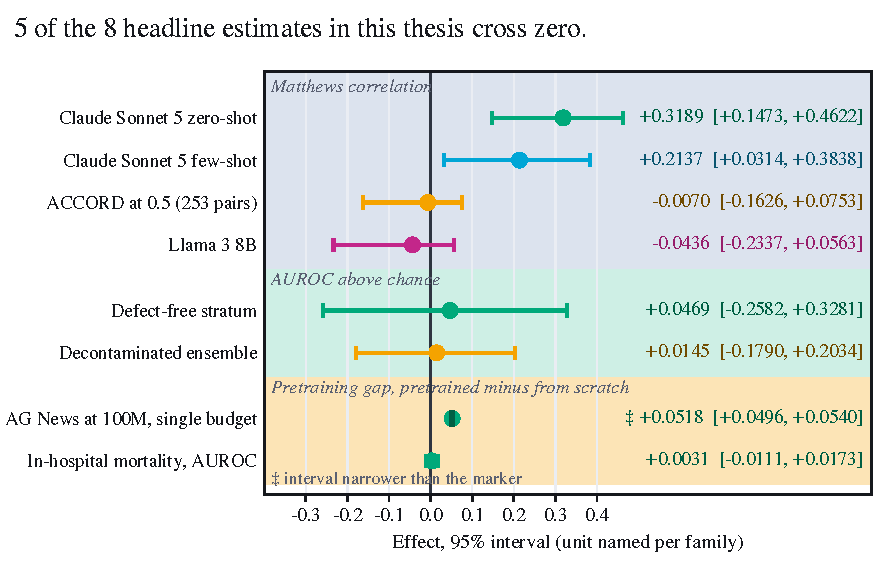
\includegraphics[width=0.98\linewidth]{figures/fig-forest.pdf}
\label{fig:forest}
\end{figure}

\subsection{Sign provenance}

Table~\ref{tab:signed} records the recomputation.

The three experiments in this subsection, the selection experiment and the two
PUMS regimes, run on simulated populations rather than the clinical pipeline,
and are retained because the sign-provenance rule they establish was
applied to the clinical numbers reported elsewhere in this thesis.

A second defect concerns direction rather than magnitude. Where a gap statistic
is stored as an absolute value, no directional claim can be recovered afterwards,
and a reader cannot tell which group a reported disparity favours. The signed
re-analysis reproduced the stored values exactly, at a maximum discrepancy of
$0.0$, which establishes that it is a faithful reproduction rather than a
different computation.

\begin{table}[H]
\caption[Signed parity endpoints, three experiments]{Signed demographic parity endpoints in three experiments.}
\centering
\small
\begin{tabular}{lrrl}
\toprule
\textbf{Experiment} & \textbf{Endpoint 1} & \textbf{Endpoint 2} &
\textbf{Sign changes} \\
\midrule
Selection experiment & $0.00841$  & $0.18939$  & none \\
PUMS, regime A       & $-0.13556$ & $-0.19435$ & none \\
PUMS, regime B       & $-0.11807$ & $-0.04101$ & none \\
\bottomrule
\end{tabular}
\apanote{Endpoint 1 is the signed gap at the weakest selection strength swept, Endpoint 2 at the strongest, not the sweep's extrema. On regime A the true minimum and maximum, $-0.20733$ and $-0.12761$, both lie outside the printed endpoints; on regime B the true minimum, $-0.12034$, is more extreme than the printed $-0.11807$, while the true maximum coincides with it. On the selection experiment both printed endpoints are the sweep's own extrema. All endpoints are reported as recorded.}
\label{tab:signed}
\end{table}

The sign analysis establishes that absolute-value storage destroys the
information a directional claim needs and that the three experiments
re-examined do not change sign inside their own sweeps; it demonstrates no
harm to any subgroup, and with 12 positives no subgroup performance claim is
supportable.

\section{Practice}
\label{sec:res-rq5}

Does the field run the checks that would have caught the failures above? This
section reports a prevalence measurement on a deliberately enriched corpus, not
a finding of the same standing as the ablation in
Section~\ref{sec:res-rq3} or the pre-registered positive control in
Section~\ref{sec:res-rq4}. It is reported because a prevalence measurement on
its own terms is worth having, and because the survey coding table of Appendix~\ref{app:survey} makes
the full 75-paper coding available for a reader to check rather than take on
trust. Of the $525$ coded fields, $502$ carry a verbatim quote checked by exact string match
against the source text, so no coded value asserting a property of a paper survives without
verified textual support. The remaining $23$ are codings of absence, recording that a paper does
not mention how it handles null attribute values; there is no sentence to quote for an absence,
and those $23$ are the \emph{not mentioned} row of Table~\ref{tab:survey}. A systematic coding of 75 papers says: rarely on the strict
reading, and not much more often on the permissive one. Both are reported side by side; the
choice between them is a judgement call for the reader.

\subsection{Both readings, and the null-attribute distribution}

\begin{table}[H]
\caption[Coded outcomes across surveyed papers]{Coded outcomes across 75 included papers.}
\centering
\small
\begin{tabular}{lr}
\toprule
\textbf{Coded outcome} & \textbf{Papers} \\
\midrule
Runs a model over the candidate pool  & 75 \\
Reports the check, permissive reading & 14 \\
Reports the check, strict reading     & 4  \\
\midrule
\multicolumn{2}{l}{\textit{Handling of null attribute values}} \\
Not mentioned     & 23 \\
Drops the rows    & 17 \\
Separate category & 13 \\
Unclear           & 9  \\
Imputes           & 7  \\
Reports only      & 6  \\
\bottomrule
\end{tabular}
\apanote{Papers are coded once each; the denominator is 75 throughout. The first row is the screening condition, satisfied by every included paper by construction. The permissive reading accepts any statement that the check was performed; the strict reading requires the quantity that would make it verifiable. The six null-attribute categories are exclusive and sum to 75.}
\label{tab:survey}
\end{table}

Four of 75 papers report the check under the strict reading and 14 under the
permissive one, so 61 report it under neither. The 10-paper gap between the two
readings is the population that says it did the check without reporting what the
check returned, and the strict count is the one a reader can verify. Twenty-three
papers, the largest single category, do not mention the null-attribute question
and nine more are coded unclear, so 32 of 75 give a reader no way to tell what
happened to rows with a missing attribute. Dropping and imputing are not
equivalent and neither is neutral, and the two choices move a reported disparity
in different directions; 17 papers take the first and 7 the second. The point is
not that one choice is wrong; it is that 32 of 75 leave it unrecoverable.

\subsection{Reliability}

One coder coded all 75 papers under the shared written rule set described in
Chapter~\ref{ch:method}. A blind second coder independently re-coded a
19-paper subsample, given the field definitions but not the hypothesis, and
that subsample is the basis for every agreement figure in this section; no
agreement is claimed for the remaining $75 - 19 = 56$ papers, which were coded
once. On the permissive cell agreement is $0.9474$ and Cohen's kappa is
$0.855$; on the
null-attribute-handling coding agreement is $0.7895$ and kappa is $0.730$.

The strict cell has no defined agreement coefficient, for a structural
reason: chance-corrected agreement
\citep{cohen1960kappa} is a ratio whose denominator is one minus expected
agreement, and when a coder's marginal on a category is degenerate that
denominator goes to zero and the coefficient is undefined rather than perfect. At
4 positive codes in 75 the strict cell is degenerate on the double-coded
subsample specifically: on the 19 overlap papers neither coder found a
strict-positive paper, so agreement is $1.0$ but kappa is undefined rather
than perfect. Reporting perfect agreement as a defined kappa would be exactly
the error the statistic exists to prevent.

The corpus is enriched, and the enrichment runs against the finding rather
than for it: a corpus that over-samples work already attentive to these
questions still yields 4 of 75 strictly, which bounds the bias without
turning 75 papers into a population estimate for the field.

% ============================================================================
%  Chapter 5. Discussion
%  \input file for a 12pt double-spaced `report' document.
%  Preamble must provide: booktabs, float (for [H]), amsmath, natbib.
%  Bibliography: accord/thesis/refs.bib
%  Numeric provenance: every quantity is from results/accord/VERIFIED_FACTS.json.
%  Compute figures come from results/accord/control_cost_log.json, the source
%  named for that item alone. No open markers remain in this chapter.
%
%  Figures: fig:forest (evaluation survived, second family), fig:scaling (the null is a
%  measurement). Sources for each are in figures/manifest.json and the
%  generating scripts beside it. The actionability timeline and the exchange-rate
%  figure were removed; the sentence and paragraph that carried their claims stayed
%  in prose. The threshold-surface figure for the
%  selection-channel anomaly moved with the rest of Section 5.3's detail to
%  the supplementary file; see the pointer at the end of that section.
% ============================================================================

\chapter{Discussion}
\label{ch:discussion}

Chapter~\ref{ch:results} reported what each stage of the pipeline measured, and
what the control attached to that stage measured afterwards. This chapter argues
about the difference. Three claims are defended: the controls changed the reading
at every stage and reversed it at several; the training and evaluation harness
resolves real differences at the sample sizes it was given, and the
twelve-positive contradiction evaluation's own sensitivity, fixed by its class
counts rather than by the harness, is a separate and narrower question the
harness result does not by itself answer; and one result here is unexplained
and should stay unexplained
until somebody tests a mechanism rather than proposing one.

\section{What Each Control Changed}
\label{sec:disc-spine}

Table~\ref{tab:disc-spine} is the summary this section argues through.

The pipeline has four stages and a reporting layer. Each produced a number a
competent paper could have reported, and no standard metric at that stage was
sensitive to the defect sitting behind the number; each was then subjected to
a control, cheap against what it checked, that was. The controls are not new: negative
controls come from observational epidemiology \citep{lipsitch2010negative}, with the positive
direction adapted here rather than taken from that source,
randomisation sanity checks from the interpretability literature
\citep{adebayo2018sanity}, control tasks and selectivity from probing
\citep{hewitt2019control}, and auditing a pipeline stage by stage has been
demonstrated for fairness in tabular preprocessing
\citep{biswas2021fairpreprocessing}. What is new is that they were run here, and
what they returned.

\begin{table}[H]
\centering
\caption[Each pipeline stage before and after control]{Each pipeline stage, the reading available before its control, and the
reading after. ``Reversed'' means the direction of the conclusion changed.
``Narrowed'' means it survived in a smaller form. ``Survived'' means the control
fired and the original reading held.}
\label{tab:disc-spine}
\small
\begin{tabular}{p{0.18\linewidth}p{0.25\linewidth}p{0.25\linewidth}p{0.14\linewidth}}
\toprule
\textbf{Stage} & \textbf{Before control} & \textbf{After control}
& \textbf{Verdict} \\
\midrule
Candidate mining & Pool base rate $0.0401$ read as a property of the mining rules & $0.0401$ is an upper bound on annotation validity, not an estimate of pool quality & Narrowed \\
\addlinespace
Weak supervision & A high-recall labeller usable in place of expert annotation & $261$ of $299$ gold pairs labelled positive against $12$ true positives; a prior, not a decision & Reversed \\
\addlinespace
Architecture & Three named components credited with the reported performance & Three different failures, not one: the authority scalars are falsified, sitting at initialisation across seeds; the rule-type head is confounded, its metric vacated by a target one linear layer from an input feature that equals it; the harm head is vacuous, with no term in the objective to train it. No randomisation control was run on any of the three & Reversed \\
\addlinespace
Evaluation & AUROC near chance, plausibly an artifact of a small and defective sample & At chance on the defect-free stratum, with an instrument shown to resolve $4.53$ points where an effect existed & Survived \\
\addlinespace
Reporting & Drift slopes read directionally from stored gap magnitudes & Same magnitudes, reproduced to a maximum discrepancy of $0.0$; roughly half the slope signs invert & Reversed \\
\bottomrule
\end{tabular}
\end{table}

\subsection{Candidate mining: narrowed}

The miner produced a pool whose base rate against pharmacist annotation is $0.0401$, $12$ true
contradictions in the $299$-pair full annotated set; on the $253$-pair decontaminated core the same
$12$ positives sit against $241$ negatives for a base rate of $0.0474$, and ACCORD thresholded at
$0.5$ on that core returns $11$ true positives against $223$ false positives, a precision of
$0.047$ that is the detector's confusion matrix rather than a further reading of pool quality.
Neither figure is a property of the annotation exercise on its own: for action-conflict candidates
the trigger quantified over sets of medication mentions while the exemplar selector indexed
positionally, and the audit found the two did not reliably agree. A reconstruction of the exemplar,
at $0.8934$ to $0.9508$ fidelity, resolves $137$ of the $165$ Rule 1 and Rule 2 candidates and finds
$65$ wrong, a rate of $0.4745$; a true key join covers only $23$ of those rows and finds all $23$
correct. The two cannot both describe the same rows, so they are reported as mutually exclusive
rather than as a range \citep{jacobs2021measurement}, and the direction of the resulting bound on
pool precision is unknown: the pharmacist judged the material shown, not corrected material, so a
higher and a lower true precision both remain consistent with the record. One stratum escapes the
defect entirely, Rule 3 and Rule 4, correct by construction, holding $134$ pairs and $6$ of the
$12$ confirmed contradictions, corroborating $0.0401$ on ground the exemplar defect cannot reach.

\subsection{Weak supervision: a prior confirmed locally, a scaling claim now withdrawn}

The labeller looked usable on the property it was checked against, recall. The control is the one
Feinstein and Cicchetti described for a different instrument thirty-six years ago
\citep{feinstein1990paradoxes,cicchetti1990resolving}: compare the marginal against a
human-established base rate before believing anything about agreement. Against the $299$ annotated
pairs the deployed local labeller assigned the positive class to $261$; the pharmacist assigned it
to $12$. Saying yes to $87\%$ of a pool whose true positive rate is $4\%$ is not a decision, it is a
prior with a text prompt attached, and three further local eight-billion-parameter models reproduce
the same miscalibration at over-calling ratios from $15.8196$ to $23.5959$
(Chapter~\ref{ch:results}), so this is not one model misbehaving. Correcting a marginal this biased
needs gold labels on the same distribution \citep{forman2008quantifying,egami2023surrogates}, which
a workflow built to avoid annotation cannot supply, so the student inherits the marginal rather
than the task \citep{ratner2016dataprogramming,ratner2017snorkel,zhang2022wssurvey}. What this
finding cannot now say is how that prior scales with capability, vendor or serving channel: the
comparisons built to answer that sent sentence pairs to hosted services, and every number they
produced has been withdrawn with the comparisons themselves (Section~\ref{sec:m-ethics}); the
question is indeterminate rather than resolved in either direction. The surviving claim is
narrower than the one this section once made: not that language models cannot reason about
clinical text, but that this project's weak labeller's marginal was a property nobody checked
before training on it \citep{pangakis2023validation}.

\subsection{Architecture: three components, three different failures}

The architectural checks did the most damage, and the word for what they did differs by component,
because no randomisation control was run on any of the three clinical components; the
randomised-substitute arms in this thesis belong to a second, provenance-conditioned system and do
not transfer here. Only the authority scalars are falsified in the strict sense: the parameter is
initialised at the value later reported as discovered, sits behind a normalisation that removes its
gradient, and agrees across seeds, so the claim that training found it is refuted. The rule-type
head is confounded rather than falsified, its auxiliary target readable from the input features one
linear layer away, the textbook symptom of leakage rather than learning \citep{kaufman2012leakage},
which vacates the metric rather than refuting the component. The harm head is neither, because no
term in the objective trains it, so no mechanism ever asserted anything a control could refute, and
its severity claim is withdrawn as vacuous. A fourth check, targeting the pretraining collapse
rather than the architecture, tested whether anisotropy rather than clinical homogeneity explains a
high similarity score: unrelated non-clinical sentences return a mean pairwise similarity of
$0.9113$ against $0.9176$ on matched clinical pairs, a Welch test rejecting exact equality
($t = 4.0001$, Cohen's $d = 0.2808$), which undercuts the homogeneity account without establishing
identity. A component credited by a system's own authors and never given a substitute that should
not work, the control-task logic \citet{hewitt2019control} developed and this thesis applies rather
than invents, has simply not been tested.

\subsection{Evaluation: survived}

The detector's ranking is at chance and stays there under every control applied to it, which is why
this thesis has a finding rather than only a list of retractions. The decontaminated ACCORD
ensemble reaches AUROC $0.5145$ ($p = 0.8668$) on the $253$ non-ambiguous pairs against $0.4595$
for the contaminated released run; the leaked rows carried the weak labeller's labels rather than
the pharmacist's, so the leak had no channel to inflate agreement with gold, making the contaminated
figure a conservative rather than an inflated comparator, and the $0.0550$ gap carries no
significance claim since no paired comparison exists in the released record. A separate,
defect-free control model, a plain BioMedBERT with none of ACCORD's authority parameters, rule
head or harm head, reaches a three-seed mean AUROC of $0.4967 \pm 0.0350$ on all $299$ pairs
(ensemble $0.4692$) and $0.5295 \pm 0.0158$ on the $134$-pair Rule 3 and Rule 4 stratum (ensemble
$0.5469$); ACCORD's own contaminated run, rescored there, reads $0.4602$ and $0.5078$, so the
control ensemble sits $0.0090$ above it at $p = 0.9300$ on the full set and $0.0391$ above it at
$p = 0.4306$ on the stratum, every interval straddling chance (Figure~\ref{fig:forest}, second
family). The stratum check has almost no power, since $6$ positives put its minimum detectable
AUROC at $0.8058$ and only the contaminated ACCORD score exists there, so the objection that real
signal was attenuated by wrong-evidence labels is not answered directly. Two baselines finish the
picture: a majority-class predictor gives AUROC $0.5$ and average precision $0.0401$, the base
rate, and a TF-IDF logistic regression gives AUROC $0.5761$, average precision $0.1571$, placing
$2$ true positives in its top $15$ where the neural detector places $0$; neither model is useful,
but no reading survives in which the custom architecture contributed something a bag-of-words
baseline could not.

\subsection{What survived}

Two things survived their controls, and a section in which nothing survives is not a finding. The
chance-level ranking survived decontamination, seed variation, defect-free stratification, a
DeLong comparison against an ensemble, and two baselines. The over-calling survived three changes
of local model family; whether it also survives a change of scale or serving vendor is now
indeterminate rather than confirmed, because the comparisons built to test that sent sentence pairs
to a hosted channel and every number they produced has been withdrawn (Section~\ref{sec:m-ethics}).
The direction of both surviving conclusions held through every correction applied to them, each of
which moved a headline number toward the negative reading rather than away from it. What did not
survive, and what the withdrawal narrows further still, is any claim about mechanism or about
scale: this is a measurement of a pipeline, not an account of why clinical text is hard or of how
the failure would change at a different model size.

\section{What the Positive Control Licenses, and What It Does Not}
\label{sec:disc-null}

A negative result in a small clinical sample invites one objection above all
others: the experiment was too small to see anything, so it saw nothing. That
objection is correct about most such results, and would be correct about this one
if no positive control existed. One does. The device adapts the one
\citet{lipsitch2010negative} formalise for observational research: run the
analysis on a case where the answer is known in advance, and let the result
speak about the instrument rather than about the substantive question.

The instrument is a comparison of a domain-pretrained encoder against an
identically sized encoder trained from scratch, evaluated by a convergence sweep
of $48$ runs. On a public four-class news classification task it resolves a
pretraining benefit of $4.53$ points at $24$ epochs: $0.9379$ for the pretrained
arm at SD $0.0029$ against $0.8925$ for the scratch arm at SD $0.0004$. The bands
are disjoint by a wide margin. At $3$ epochs the gap is $5.07$ points, so the
effect is present early and does not depend on the budget chosen.

The budget is what closes the objection. Eight times the training budget bought
the 100M-parameter scratch arm $0.41$ points, from $0.8885$ at $3$ epochs to $0.8925$
at $24$; the pretrained arm moved $-0.13$ points over the same range. Both arms
are converged. A gap that persists at convergence is not a gap in optimisation,
and an instrument reporting a $4.53$-point difference at standard deviations
at or below $0.0036$ is not an instrument that cannot see effects.

Parameters do not close it either. Table~\ref{tab:scaling} reports the from-scratch
arms at three sizes against the pretrained band on the public task. The
from-scratch curve rises with size and does not approach the band, so the public
gap is a pretraining effect rather than a capacity effect, and the mortality
control returns almost nothing (Figure~\ref{fig:forest}, last row).


The decision rule was committed before the sweep ran, at repository commit
\texttt{b048829}, and the outcome it adjudicated
is the one that keeps the claim rather than the one that discards it. That
ordering is the whole value of pre-registration, and it could have gone the other
way: arms that had not converged would have retired the positive control and with
it the licence to call the mortality-control result a measurement. On the
mortality control task, in-hospital mortality predicted from a patient's first
$48$ hours of notes on $6{,}776$ held-out admissions holding $570$ positives, the
same instrument, harness and protocol return $+0.0031$, with the pretrained arm
at $0.7693$ (SD $0.0102$) against $0.7662$ (SD $0.0073$), each at three seeds.
No significance test for that difference is registered, so no $p$ value is
quoted; the two standard deviations alone make the gap look like noise around a
shared value rather than a resolved difference, and the sign is not robust:
restricting the from-scratch arm to the two runs whose data lineage is recorded
gives $0.7703$ and a gap of $-0.0011$. Both readings are nulls and the argument
below turns on neither. Same instrument, same protocol, two tasks, one
showing $4.53$ points and the other showing nothing.

The general result is not this thesis's. Pretraining loss is a poor proxy for
downstream performance, and that is settled at far larger scale than $48$ runs
\citep{lourie2025scaling,feng2026tessera}. The
sweep here is a positive control for the mortality-task measurement, and writing
it up as a contribution would misrepresent what it is for.

What this control licenses is narrower than it can sound: that the harness
resolves a real difference at the sample sizes it was given, not the
sensitivity of the twelve-positive contradiction evaluation, a different
instrument with its own minimum detectable AUROC, $0.7355$ at $12$ positives
against $241$ negatives ($0.7350$ on the $299$-pair set, $0.8058$ on the
$6$-positive defect-free stratum), fixed by that evaluation's class counts and
corroborated arithmetically by simulation in Chapter~\ref{ch:results}. This work
therefore cannot establish that cross-note medication contradiction detection
is unsolvable; it establishes that this pipeline does not solve it, and that an
effect at or above $0.7355$ would have been visible had one been present. Only
the second statement is made.

A bootstrap standard deviation of $0.0870$ on the contaminated released run's
$G_{299}$ AUROC is consistent
with a mildly informative model and with a mildly inverted one. The three-seed
ensemble's own $95\%$ bootstrap interval on the $253$-pair set,
$[0.3210, 0.7034]$, is wide enough that its upper bound of $0.7034$ sits only
$0.0321$ below the minimum detectable AUROC of $0.7355$, so interval width on its own does not rule out a
modestly useful model. Three of the four estimators compared here, the single
model, the three-seed ensemble and the TF-IDF baseline, could in principle have
found separation and did not; the fourth, a majority-class predictor, returns
AUROC $0.5$ by construction and was never in a position to look, so it is a
reference point rather than a fourth line of evidence. What the three estimators
that could fail and did not agree on is the evidence a sample this size can
produce, not proof that no separation exists.

\section{An Anomaly, Reported as an Anomaly}
\label{sec:disc-anomaly}

One result here is not explained, and this section reports it without
explaining it. It is not counted among Chapter~\ref{ch:intro}'s
contributions, and that billing is deliberate rather than an oversight: a
contribution earns its place by explaining something, and this pattern
explains nothing about itself. The population audited is simulated, not the
clinical pipeline; it is retained because the same experiments also anchor
the sign-provenance rule of Chapter~\ref{ch:results}, applied afterward to
the clinical numbers, and because a pattern that does not fit is better
reported than dropped.

On two simulated populations, with baseline disparity held fixed, upstream
selection channels were swept and the pool-level demographic parity gap
audited at each step. The gap never changes sign within a sweep, but the
direction it drifts in does: two channels swept on the same population give
fitted drift slopes of opposite sign, and on the population where the sweep
was extended across operating points as well as channel strength, the
audited gap moves with both, so a single audited number describes one cell of
a surface rather than the system that produced it. A further, controlled
sweep of the same construct across baselines, channel strengths and
replicates does not reproduce even that channel dependence: it inverts the
mapping between channel and drift direction, so the direction a pool audit
drifts in is not a stable function of the channel that produced it, at least
across the region examined.

Five mechanism claims were proposed during this project to account for this
pattern; each was tested against a parameter sweep and each failed, and a
sixth is not offered. No subgroup harm is demonstrated, none is demonstrated
anywhere in this work, and no general claim is made that disaggregated
fairness evaluation is uninterpretable under selection; that argument belongs
to others and predates this work
\citep{pfohl2025disaggregated,fogliato2020fairness}, as does the observation
that the design choices inside a disaggregated evaluation are consequential
enough to need documenting \citep{barocas2021disaggregated}. The full sweep,
the operating-point surface, and the failed mechanism accounts are given in
Appendix~\ref{app:anomaly}.

\section{Measurement Provenance}
\label{sec:disc-provenance}

Every disparity gap in this project was stored as an absolute value, and most
ratio quantities as a minimum over a maximum, with no per-group values persisted.
Each decision is individually reasonable: a magnitude is the right object for a
pass or fail check against a tolerance. Together they destroy the information
every directional sentence in the analysis depended on.

The retrofit is the useful part. Signed storage was added alongside the existing
fields rather than replacing them, and the recomputation reproduced every prior
value with a maximum discrepancy of $0.0$; the reproduction check passes. Nothing
previously reported changed by any amount. What changed was the sign of roughly
half the drift slopes, and one credibility call: a slope whose stored interval
crossed zero has a signed interval that does not. The flip count reported here, $7$ of $14$
compared metric-slopes, is the figure carried into the verified register
(Appendix~\ref{app:corrections}, C57). The field count behind the retrofit is not registered and
is not quoted.

The rule is one sentence. A metric stored as a magnitude licenses no directional
claim, and no downstream care recovers what the storage discarded. It is not
novel and should not be dressed as novel; it is a specific case of a general
point about measurement provenance and about the debt that accumulates when an
intermediate representation is chosen for one consumer and read by another
\citep{sculley2015debt}. What this work adds is a demonstrated true positive.
Applied to this project's own artifacts, the check invalidated four directional
readings, three of which were themselves corrections of earlier errors. A rule
that catches a correcting analysis committing the error it is correcting has some
claim on a practitioner's attention. Two qualifications: the check is cheap only
because these sweeps were cheap, and where per-group values were never written
the retrofit is a re-run rather than a recomputation; and the demonstration is on
one project's artifacts, so no claim is made about how often the defect occurs
elsewhere.

\subsection{What practice does with the upstream check}

The survey speaks to whether the check that would have caught the upstream defect
is run at all. Auditing a pipeline one stage at a time is not an exotic ask:
\citet{biswas2021fairpreprocessing} do it for tabular preprocessing operators,
and show that the local behaviour of each stage composes into the behaviour of
the pipeline. On a $75$-paper corpus, $4$ papers audit the selection step under
the strict reading and $14$ under the permissive one, so $61$ report it under
neither. What those $61$ do instead is not recorded by this coding, which asks
only whether the check appears; a separate coded field, how each paper handles
null attribute values, is reported over the same $75$ papers in
Table~\ref{tab:survey}, and the two fields are different variables on the same
corpus rather than a partition of it.

Both readings appear because the coding cannot separate them cleanly, and
reporting only the one that suits the argument would be the error this thesis is
about. The corpus was deliberately enriched for fairness-forward work, and the
enrichment runs against the finding rather than for it: a corpus over-sampling
the papers most likely to run the check still returns $4$ of $75$ strictly. This
is not a prevalence estimate for clinical machine learning. Coverage is
open-access and preprint venues rather than the literature as a whole, and
$459$ screened-in papers were never retrieved in full text.

\section{What the Controls Cost}

Table~\ref{tab:disc-cost} itemises it.
\label{sec:disc-cost}

Nobody reports this, so it is reported here, with the limit stated first.
\textbf{These figures are compute only.} Person-hours were not logged for most
of the project and are not reconstructed, because a reconstructed estimate
would be an invented number in a thesis about invented numbers.

\begin{table}[H]
\centering
\caption[Recorded compute cost of controls]{Recorded compute for the controls. Person-hours are excluded and were
not logged. The cost log records a $12$-run, $34.9$-minute public-task episode
but omits the $48$-run, $555$-minute convergence sweep the argument in
Section~\ref{sec:disc-null} rests on. The two are separate run sets, not one
nested in the other: nine of the twelve cells differ from the convergence
sweep's shortest-budget cells and all twelve recorded runtimes differ, so both
are counted here.}
\label{tab:disc-cost}
\begin{tabular}{lrr}
\toprule
\textbf{Control episode} & \textbf{Runs} & \textbf{GPU-minutes} \\
\midrule
Public-task convergence sweep             & 48 & 555.0 \\
Public task, single budget across scales  & 12 & 34.9 \\
Clinical task, pretrained against scratch & 17 & 612.3 \\
Signed re-run, selection experiment       & 1  & 0.7 \\
Signed re-run, PUMS replication           & 1  & 13.5 \\
\midrule
Total, reconciled                         & 79 & 1216.4 \\
\bottomrule
\end{tabular}
\end{table}

The control that retracted the directional core of three corrections cost
$0.7 + 13.5 = 14.2$ GPU-minutes across both experiments. The convergence sweep that licenses the
whole argument of Section~\ref{sec:disc-null} cost $555$ minutes on its own. Together with the
clinical-task comparison the two larger sweeps cost $555 + 612.3 = 1167.3$
GPU-minutes, and the reconciled total is $555 + 34.9 + 612.3 + 14.2 = 1216.4$
GPU-minutes and $79$ runs in total, roughly twenty GPU-hours. The claim is not that
controls are always cheap: re-annotation is not, a second annotator is not, and
the one control here that cannot be recomputed from disk requires re-running the
experiment that produced it. The claim is narrower. In this project the controls
that reversed conclusions cost less compute than the experiments whose
conclusions they reversed, and cost is not why they went unrun.

No comparison against prose checklists is offered. An earlier version of this
work compared executable gates against checklist-style review, and that
comparison was retracted: the gate recorded no failure in any run, so its catch
rate is undefined, while the checklist arm computed the relevant defect, wrote it
to disk, and was misread by a human. Executability was not the binding
constraint, and no claim is made that executable gates outperform prose
checklists. The nearest thing to evidence on that question comes from journal
peer review rather than from here, where introducing an automated statistical
consistency check is associated with a steep decline in reporting
inconsistencies \citep{nuijten2023statcheck}, measured over a corpus this
project cannot approach.

\section{Limitations}
\label{sec:disc-limits}

\paragraph{RQ4's answer, now that the hosted channel is ruled out.} One dependency in this thesis
ran through four chapters and is stated here as a settled finding rather than a hypothetical,
because the question it depended on has been answered rather than left open. Section~\ref{sec:m-ethics}
records that every hosted-service transmission this project made, on the Anthropic API and on AWS
Bedrock alike, has been withdrawn: PhysioNet's guidance of 24 September 2025 prohibits third-party
retention without a vendor qualifier, and every hosted route used here transmitted credentialed
sentence pairs off the analysis machine, so every number those runs produced has been removed from
the set a reported figure may resolve against. Those rows, not the local eight-billion-parameter
models, were the evidence that the twelve-positive contradiction evaluation could resolve an effect
at all, so Section~\ref{sec:r-frontier}'s demonstration reverts to the calculation it was built to
replace, and RQ4's answer moves from ``the instrument was sensitive enough to see an effect of that
size'' to ``the minimum detectable effect says an effect of that size should have been visible, and
nothing that remains in the register confirms that one was.'' No vendor-specific fallback survives
this: an earlier reading of this dependency distinguished Amazon Bedrock, on the retention test
PhysioNet's guidance sets out, from the Anthropic API, but the withdrawal recorded in
Section~\ref{sec:m-ethics} applies uniformly to every hosted route used here, so that distinction no
longer has anything left to save. What still stands is the pretraining positive control, which
shows the same measurement apparatus resolves a real difference on a public benchmark unconnected
to any hosted transmission, and the rule-head transfer collapse, neither of which touches a hosted
API. That is a weaker position than an earlier version of this chapter argued from, and it is the
position this thesis now holds.

The limitations below are stated without hedging. Several are severe enough that
a reader could reasonably decline to draw a conclusion from part of this work,
and where that is so it is said.

\paragraph{Twelve positives.} Every ranking measurement rests on $12$ positive
cases, and the defect-free stratum on $6$. The minimum detectable AUROC at $80\%$
power is $0.7355$ on the primary set and $0.8058$ on the stratum. The intervals
are wide and the ordering between the two systems this pipeline produced is
unidentified, their Matthews correlations being $-0.0436$ and $-0.0070$, both
within $0.05$ of chance. The limit is not that $12$ positives cannot separate
anything: two of the local weak-labeller replicates from
Section~\ref{sec:m-control-rq2}, \texttt{granite3.3:8b} zero-shot and
\texttt{llama3:8b} few-shot, carry Matthews correlation intervals against these
same $253$ rows that exclude zero, at $0.1326$ and $0.0540$. That is a claim
about those two labeller configurations on the agreement-with-gold question, not
about the contradiction detector, and the qualification belongs in the same
breath as the claim rather than later: $12$ positives can separate a system from
chance when the effect is large enough, so the null the detector and its control
return is a statement about those two architectures, which sit close to chance
and to each other, rather than a statement that no instrument at this sample
size could ever resolve anything. No ablation carries a significance claim.

\paragraph{Deployment risk, and automation bias.} A system with recall
$0.7778$ and precision $0.0424$ generates a large number of false alarms per
true contradiction: the decontaminated detector's first seed alone raises
$216$ false alarms against $9$ true contradictions. Alert burdens at that
ratio are associated with reduced acceptance
\citep{vandersijs2006overriding,ancker2017alertfatigue}, so this system should
not be deployed in any form; its failure mode is worse than doing nothing, since it consumes
clinician attention while providing no information. A second, more specific
hazard sits inside the architecture: the harm head of
Section~\ref{sec:m-detector} received no loss term and its outputs span
$0.3977$ to $0.6096$, an untrained sigmoid's range, yet an earlier version of
this work presented that output as a severity score, a plausible danger
score derived from random initialisation, the specific and most serious
instance of automation bias this project produced. The diagnostic that
catches it, printing the empirical range of every emitted score, costs one
line.

\paragraph{One institution, one corpus, one era.} MIMIC-III covers admissions to
a single United States academic medical centre \citep{johnson2016mimic}. The
primary cohort is a billing-code phenotype, over-including admissions where the
condition is a comorbidity and under-including those where it was present and
uncoded. Documentation conventions, note-type taxonomies and medication-list
formatting are institution- and era-specific, and the drug dictionary, class
dictionary, dose threshold and danger judgements all encode that context. The
transfer cohorts move across index diagnosis within the same institution, so
nothing speaks to cross-institutional generalisation
\citep{zech2018generalization}. MIMIC-III is a credentialed PhysioNet resource;
all analysis reports aggregates only, and no clinical note text and no
identifiers appear in this document or in any released artifact.

\paragraph{The trigger fires late, and the record cannot say how late.} The
system compares a nursing note against a discharge summary, so it produces
nothing until the discharge summary exists, and that document closes the
admission rather than preceding it, finalised at or after discharge rather than
before it. The data model compounds the problem: nursing notes carry a
charting timestamp and discharge summaries carry only a charting date, so the
summary cannot be placed in time relative to the discharge itself. That same
field absence is what invalidated an earlier prefilter result in this project,
retracted in Appendix~\ref{app:corrections}. A contradiction detected at that
point is a documentation finding rather than an intervention, and a deployment
claim would have to move the trigger earlier, to the discharge order rather than
to the finished summary. Nothing here measures whether the task is tractable at
that earlier point, and nothing here should be read as a claim that it is.

\paragraph{The exemplar defect bounds annotation validity, and re-annotation was
not performed.} This is the limitation most likely to be read as smaller than it
is. The rebuild that corrects the selector exists; the re-annotation that would
convert the bound of Section~\ref{sec:disc-spine} into an estimate was not run.
So $0.0401$ cannot be cited as a property of the mining rules by anyone, this
thesis included, and a reader who wants that quantity should treat it as
unmeasured rather than as measured with error. What the defect does not touch is
the central evaluation result, which reproduces on the $134$-pair stratum. The
defect-free stratum, correct by construction, offers a check that does not
depend on that estimate: it holds $6$ of the $12$ confirmed contradictions in
$134$ pairs, a rate of $0.0448$, corroborating $0.0401$ on a stratum where the
exemplar defect cannot fire. The weak-supervision finding needs no base-rate
estimate at all: $261$ of the $299$ gold pairs were labelled positive against
$12$ confirmed, a marginal comparison with no denominator to estimate.

\paragraph{The survey is a prevalence measurement on an enriched corpus, and it
is limited on several axes at once.} It is the weakest of the empirical
strands in this thesis, reported at that weight rather than alongside the
ablation or the pre-registered convergence control. The $75$-paper corpus was
assembled to over-sample fairness-forward work, coverage is open-access
sources only, $459$ screened-in papers were never retrieved in full text, and
one coder codes the full set; Chapter~\ref{ch:results} gives the full
enrichment argument behind $4/75$ and $14/75$. A blind second coder recoded a
subsample with field definitions only and the hypothesis withheld, and
agreement on the permissive field is high. On the 19 double-coded papers, the
registered permissive
agreement is $0.9474$ with kappa $0.855$. On the strict cell, the one that decides the
headline count, the reliability coefficient is
\textbf{undefined}: both coders returned the same code on all 19 overlap
papers, which drives a coder's marginal on the category toward degenerate and
the denominator of a chance-corrected coefficient toward zero. The full
contingency table behind the undefinedness is not registered and is not
claimed here beyond that. It is reported as undefined rather than as the
perfect agreement the raw agreement rate superficially permits, which is the
same class of error as reporting a coefficient guaranteed by construction.
The survey coding table of Appendix~\ref{app:survey} reproduces the full 75-paper coding, so a
reader who wants to check the count rather than take it on trust can.

\paragraph{One annotator, and the reliability figure this instrument cannot
produce.} Every gold label came from a single board-certified
pharmacist in two passes separated by a washout. The washout controls
within-session drift; it does not establish inter-rater reliability, because
there is one rater. A previously reported perfect agreement between two
``independent judgement instruments'' is retracted in
Appendix~\ref{app:corrections}: the instruments were logically equivalent, so the
coefficient was guaranteed by construction \citep{cohen1960kappa}. Nor does the
washout supply an intra-rater figure by another route: the two passes were not
retained as separate columns, the second overwrote the first in the annotation
record, and no committed artifact holds pass-one and pass-two labels side by
side. The absence is not a reporting gap that a re-run of an existing script
would close. It is a property of what the record kept. No inter-rater or
intra-rater agreement statistic exists for the 299-pair gold standard, one
cannot be recovered from the two-pass design, and every clinical result in this
thesis, the pool precision, the weak-labeller comparison, the detector's AUROC,
the danger ratings, rests on that unmeasured instrument. Board certification is
a credential, not a reliability coefficient, and it is not offered as one here.

\paragraph{No rate is claimed from the correction record.} The self-audit record
is an appendix and a demonstration, not a statistic. An attempt to compute an
error rate from it was retracted: the generating script was not saved, the
denominator advanced without the numerator, and an independent hand-code
intersected the original list on a minority of the union. The record supports
named instances, including four cases of a correcting analysis committing the
error it was correcting.

\section{Threats to Validity}
\label{sec:disc-threats}

Internal threats attack whether the measured relationships hold in this sample,
external threats whether they hold anywhere else, construct threats whether the
quantities measured are the quantities named. They are separated because they
call for different responses.

\subsection{Internal validity}

Table~\ref{tab:disc-internal} lists them and what this thesis does with each.

\begin{table}[H]
\centering
\caption[Internal threats and their status]{Internal threats and what this thesis does with each. Two are bounded by
measurement; the rest are stated rather than argued away.}
\label{tab:disc-internal}
\small
\begin{tabular}{p{0.28\linewidth}p{0.22\linewidth}p{0.36\linewidth}}
\toprule
\textbf{Threat} & \textbf{Severity} & \textbf{Status} \\
\midrule
Twelve positives; every interval wide & Severe & Stated; MDE $0.7355$ reported with every null; no significance claim on any ablation \\
\addlinespace
Training contamination of the evaluation set & Severe if unaddressed & Measured and corrected; the decontaminated ensemble is $0.5145$ against $0.4595$ contaminated, so the correction does not favour the conclusion \\
\addlinespace
Exemplar defect on action-conflict candidates & Severe for pool precision, not decisive for the central result & Checked on the defect-free stratum by a separate control model, not a rescoring of the decontaminated ACCORD: $n = 134$, $6$ positives, three-seed ensemble AUROC $0.5469$, $95\%$ bootstrap interval $0.2418$ to $0.8281$, MDE $0.8058$. ACCORD's contaminated released run reads $0.5078$ on the same rows; no decontaminated ACCORD score exists there \\
\addlinespace
Single annotator, no inter-rater or intra-rater reliability & Severe; bounds every gold-label conclusion & Stated; the earlier circular coefficient is retracted, and the two-pass design cannot recover an intra-rater figure because the passes were not retained separately \\
\addlinespace
Weak-label leakage into model inputs & Moderate to severe & Demonstrated on the rule-type head, whose target is one linear layer from an input feature that equals it; the affected metric is vacated, which leaves the head untested rather than falsified \\
\addlinespace
Extraction never validated against human annotation & Moderate to severe; no downstream error rate decomposes & Stated; first item of any continuation \\
\bottomrule
\end{tabular}
\end{table}

The contamination row deserves a sentence, because the direction of a correction
matters. A correction that improves the result it corrects invites the suspicion
that it was selected; every correction applied to a headline number here moved it
toward the negative conclusion, which is weak evidence but evidence in the right
direction.

\subsection{External validity}

Generalisation is bounded on four axes. One centre and one documentation culture.
One primary billing-code phenotype, with two weaker transfer cohorts that move
across index diagnosis rather than across sites. One era, predating current
documentation systems and any use of generative assistance in note writing. The
fourth axis is the task, and there the bound is measured rather than assumed: the
over-calling magnitude does not generalise, because a control on public text
returned a much smaller factor for the same labellers, and the part that
transfers is the mechanism, a labeller reporting a prior when the base rate is
low; the public-text maximum over-calling ratio, measured on SNLI across three
models, two prompts and four prevalence levels, is $3.5000$, well
below the $15.8196$ to $23.5959$ range measured on the clinical pool.
The positive control is external evidence of a
limited kind: it shows the instrument behaves as expected on a public benchmark,
and says nothing about whether the clinical result would reproduce elsewhere.

\subsection{Construct validity}

Four constructs are named more confidently than they are measured, which is the
gap between a construct and its operationalisation that
\citet{jacobs2021measurement} argue is where invalid conclusions originate.
``Dangerous medication contradiction'' is operationalised by four rules and one
pharmacist's judgement; a different reading of what counts as a conflict yields a
different pool and plausibly a different base rate, and the construct is not
independently validated. The detector's target is the weak label, not the
clinical event, so any statement that it ``fails to detect contradictions'' is a
statement about what it learned to predict. Ranking metrics at a $4\%$ base rate
also measure less than they appear to: AUROC is insensitive to prevalence in a
way that flatters this setting, while average precision, which is not, sits near
the base rate throughout \citep{saito2015prcurve}, and agreement statistics here
are subject to the documented paradoxes
\citep{feinstein1990paradoxes,cicchetti1990resolving,byrt1993pabak}. Matthews
correlation is used as the better-behaved default
\citep{chicco2020mcc,delgado2019kappa} rather than as a solution, and applying
that critique is not contributing it; it is thirty-six years old.

The part of that critique this evaluation set makes concrete is the exchange
rate. Each summary statistic implies a rate at which a forgone true positive is
worth some number of gained true negatives, and the rate is fixed by the class
counts rather than by anything clinical. The prevalence-adjusted bias-adjusted kappa
\citep{byrt1993pabak} has the shallowest exchange of the three most commonly
reported here, which makes it the most majority-dominated of them despite the
name, and none of the three was chosen by asking what a missed contradiction
costs relative to a false alarm. That question is clinical and it was never
posed. One worked example on this evaluation set makes the point without a
figure. The local \texttt{granite3.3:8b} few-shot labeller of
Section~\ref{sec:m-control-rq2} carries a confusion matrix of $10$ true
positives and $75$ true negatives against ACCORD's $11$ true positives and
$18$ true negatives on the same $253$ rows: it trades one additional forgone
true positive for far more gained true negatives, which is worse on the
first axis and far better on the second, and Matthews correlation prices that
trade as a net gain rather than a net loss, which is why the labeller's
coefficient of $0.0668$ is positive on this set where ACCORD's $-0.0070$ is
not, even though the class counts are what move the statistic here, not a
clinical judgement of which errors matter more. The same two confusion
matrices could support opposite readings under a statistic with a different
exchange rate, so the choice of summary statistic is not a neutral reporting
convention but a decision about which errors are worth trading, taken before
any result is seen.

Finally, the
survey's coded construct admits two defensible readings, and the gap between the
strict and permissive counts is the size of that ambiguity.

Three results would change these conclusions, and they are tests rather than
hedges. Re-annotation against corrected exemplars would convert the
pool-precision bound into an estimate. A cohort with substantially more than $12$
positives would move the minimum detectable effect down far enough that a modest
true signal, if one exists, would be visible; at present a true AUROC around
$0.65$ is indistinguishable from chance in this design. An explanation of the
selection-channel anomaly that survives a parameter sweep, unlike the five that
did not, would convert Section~\ref{sec:disc-anomaly} from a report into a
finding. None is available from the data collected here.


\clearpage
\phantomsection
\addcontentsline{toc}{chapter}{References}
% References: double-spaced, no extra gap between entries. apa.bbx sets the
% APA hanging indent itself through \bibhang, so the bibliography list is NOT
% redefined here; the numeric-comp override this file used to carry keyed off
% \labelnumber, which APA does not set, and would have printed an empty label
% box and flattened the hanging indent on every entry.
\begingroup
\doublespacing
\setlength{\bibitemsep}{0pt}
\setlength{\bibparsep}{0pt}
% Page ranges print with an en dash, english.lbx's default for \bibrangedash.
% The handbook requires one in a numerical range ("1995--1998, 32--35"), and the
% project's no-dash rule is scoped to prose: verify_thesis.py pass 1 permits an
% en dash only between two digits and still fails on every other dash use.
\printbibliography[heading=bibliography]
\endgroup

% Appendices, generated from the project records by
% accord/stats/make_appendices.py so they cannot drift from the source.
\appendix
\renewcommand{\thechapter}{\Alph{chapter}}
% The table of contents is typeset in the front matter, before this point is
% reached, so redefining the prefix here would not reach it: the appendix printed
% as "Chapter A:". The switch is written into the .toc stream instead, so it fires
% where the appendix entries begin when that file is read back.
\addtocontents{toc}{\protect\renewcommand{\protect\cftchappresnum}{Appendix }}
\addtocontents{toc}{\protect\setlength{\protect\cftchapnumwidth}{6.8em}}
\titleformat{\chapter}[block]
  {\normalfont\centering\bfseries\normalsize}
  {Appendix \thechapter:}{0.5em}{}
\chapter{The Correction Record}
\label{app:corrections}

This appendix lists every correction issued during the work, in the order it was issued.
Each entry records a claim that was withdrawn, narrowed, or confirmed against evidence.
The full text of each, with its artifact and reasoning, is retained in the project
repository. The record is included because the sequence is part of the result: it shows
which conclusions moved, and what moved them.

\section{Corrections}

\singlespacing
\begin{longtable}{@{}p{0.6in}p{4.6in}@{}}
\textbf{ID} & \textbf{Correction}\\
\midrule
\endhead
C1 & The authority weights are an initialization artifact\\
C2 & Rule F1 = 0.9603 is label leakage\\
C3 & The \$ kappa\$ = 1.000 internal-consistency claim is circular\\
C4 & Three architectural components are not backed by running code\\
C5 & The contaminated set must be removed\\
C6 & The prefilter finding is an instrument failure\\
C7 & Reported "3 seeds" are 2 seeds plus a hardcoded row\\
C8 & Splits are row-level, not patient-level\\
C9 & \texttt{weak\_confidence} is degenerate\\
C10 & The multi-LLM "model-agnostic" conclusion rests on one model\\
C11 & The ethnicity disparity is a missingness artifact\\
C12 & The language finding splits, and only half survives\\
C14 & The "compounding bias" claim is withdrawn ,  the sign was produced by adjustment\\
C13 & "Clinical homogeneity" does not explain the Stage 0 collapse\\
C15 & The thesis's external-validity claim rests on a non-significant result\\
C16 & The reported evaluation appears to be the contaminated run\\
C17 & The volume adjustment controls the wrong note\\
C18 & Decontamination was row-level; 158 of 266 gold subjects were also in the training pool\\
C19 & The defect-free control result, and what it does and does not license\\
C20 & C10 repaired: the miscalibration is model-agnostic, the differential is not\\
C21 & The denominator framing survives its falsifier ,  and my earlier "already published" call was too broad\\
C22 & The pool audit "passes" partly because the audited classifier is near-constant\\
C23 & "Model-agnostic miscalibration" is refuted by a file already in the results directory\\
C24 & Both empirical legs of the lead claim are compromised\\
C25 & The era confound is closed without \texttt{ICUSTAYS.csv}, and it largely explains the effect\\
C26 & Novelty reassessed: the sweep is pre-empted, and four-fifths on a missingness flag is attackable\\
C27 & The survey's reliability holds under blind second coding\\
C28 & The real-data leg is dead: the audit is not blind, it fails almost everywhere\\
C29 & The invariance proposition is verified numerically, and the metric taxonomy is the finding\\
C30 & The rebuilt simulator can now fail, and its controls fire correctly\\
C31 & The invariance proposition is a textbook consequence. Do not claim it as theory.\\
C32 & The C4 headline comparison is on a dataset that no longer exists\\
C33 & Drive compliance remediated\\
C34 & The C4 comparison re-run on current data: the efficiency claim holds\\
C35 & The PubMed/ACL pass: Part A survives narrowed, Part B loses "disjoint"\\
C36 & E2 to E5: the intervals the thesis reported point estimates for\\
C37 & E1 complete: the small encoder is not distinguishable from PubMedBERT\\
C38 & E9 REFUTES the invariance claim in the realistic regime\\
C39 & Two errors this experiment surfaced in my own record\\
C40 & E9 is threshold-robust in the region where it can be tested, and never inverts\\
C41 & The PUMS replication confirms the clinical finding, and corrects my own taxonomy\\
C42 & The prevalence replication REFUTES the generality of the clinical over-calling result\\
C43 & C42's "distillation half is also negative" is a threshold artifact ,  measured properly, the student inherits the teacher's marginal\\
C44 & The scaling study refutes C37's generalization ,  and reframes it into a better claim\\
C45 & The DAG tests do not support my confounder lean ,  both readings stay live\\
C46 & The framing was wrong, and the experimental record is now closed\\
C47 & E9 and E10 drift in opposite directions; I fused them by discarding the sign\\
C48 & My own figure code hardcoded the values it claimed to read, and drew a power curve from an invented formula\\
C49 & The survey ,  the thesis's strongest claim ,  has no per-paper coding table on disk\\
C50 & The C47 mechanism is refuted by its own pre-registered kill condition; the sign is set by the selection channel, not the baseline\\
C51 & C41's Regime A table does not match the run it reports, and the "correction to C29" it motivated was unnecessary\\
C52 & Every gap in these experiments is absolute-valued, so no directional claim was ever licensed\\
C53 & C28's premise was wrong ,  but the investigation found a real error that flips a sign in six places\\
C54 & The 22,446,855-parameter configuration was never built, and 590,592 of it could never have received a gradient\\
C55 & The survey recode does not reproduce 0/25 and 0/4. Per C49 it governs, and the headline claim changes\\
C56 & The "opposite directions" that three corrections were built on is an artifact of \texttt{abs()}, and the simulator does not corroborate the real data\\
C57 & The drift regressions were still fitted to unsigned columns after the C52 retrofit; seven slopes flip\\
C58 & The weak labeller's MCC interval is now computed rather than asserted\\
C59 & The survey now has a reliability figure, and it does not cover the decisive cell\\
C60 & The novelty check the frame never had: both candidate framings are prior art, and the uncovered claim is one the project has been treating as an appendix\\
C61 & C40 survives the signed reading; and I swept an agent's in-flight edits into an unrelated commit for the second time\\
C62 & The C44 convergence sweep returns OUTCOME A under the pre-registered rule: the arms were converged and the control holds\\
\end{longtable}
\doublespacing

\section{Revisions After the Record Closed}

The correction record was closed once the frame was frozen. Findings after that point
change a number, a chapter, or a stated limitation, and by rule cannot change the
thesis statement. They are listed separately for that reason.

\singlespacing
\begin{longtable}{@{}p{0.6in}p{0.9in}p{3.8in}@{}}
\textbf{ID} & \textbf{Date} & \textbf{Revision}\\
\midrule
\endhead
R1 & 2026-08-10 & the self-audit statistic is retracted; it is unreproducible and wrong in membership\\
R2 & 2026-08-10 & the gate-vs-checklist comparison is retracted; its treatment arm has no positives\\
R3 & 2026-08-10 & DESIGN.md carries numbers C39 corrected\\
R4 & 2026-08-10 & the round-two novelty pass closes the self-audit frame; the general proposition is occupied in five literatures\\
R5 & 2026-08-10 & C62 is a positive control, not a contribution\\
R6 & 2026-08-10 & C54's checkpoint premise is false; 23 checkpoints exist on the Drive mount\\
R7 & 2026-08-10 & the number audit: 15 mismatches, 9 of them abstract-level; the introduction inverts the central claim\\
R8 & 2026-08-11 & three source conflicts resolved before they reached the page\\
\end{longtable}
\doublespacing


\chapter{Reference Tables}
\label{app:provenance}

Three reference tables belong to the record behind this thesis, machine-generated by
\texttt{accord/stats/make\_appendices.py} and \texttt{accord/stats/trace\_claims.py} and
reproduced complete, without abbreviation, in the supplementary file that accompanies this
document. They are bound separately because together they run to more than thirty pages of
table, none of which is read sequentially.

The first is the register of reported quantities: 1397 values, each extracted from a stored
result file by script rather than transcribed by hand, grouped by the experiment that produced
it and listed with the file it was read from. The register is what makes the claim in
Chapter~\ref{ch:method} checkable, that no figure in this document was typed from a draft, a
note, or memory.

The second is the claim and evidence trace. It resolves 1152 numeric occurrences in the
chapters against the register: 283 match a single registered value with no other candidate,
613 match one of several candidates on a shared word in the surrounding sentence, and 256
remain genuinely ambiguous, sharing a value with more than one registered quantity with
nothing in the sentence to disambiguate. The trace records that distinction per occurrence
rather than picking silently, so an ambiguous attribution stays visible as such.

The third is the survey coding table behind the prevalence measurement in
Chapter~\ref{ch:results}, 75 papers coded against a written instrument and reproduced in full
so the counts can be recomputed rather than taken on trust.

Appendix~\ref{app:corrections}, the correction record, is not in the supplement: it is written
rather than generated, and belongs with the argument.

% Side strands (second system, fairness audit validity, practice survey,
% compute cost) are not bound: the thesis is submitted as one document and no
% supplement was written. Two generated tables that used to be bound are not
% reproduced in either document, the register of reported quantities and the
% claim-and-evidence trace. Both printed an internal file path beside every
% row, which is working-notes material rather than thesis material, and both
% are released with the analysis code where they can be queried rather than
% read. Appendix A's closing section says so in words.
% The full quantitative treatment of the selection-channel anomaly is released
% with the analysis code, as the complete correction record, the register and
% the claim trace already are. The thesis reports the anomaly in summary in
% Section sec:disc-anomaly and states that it is not a finding, so an appendix
% of its sweep carried no claim the text depends on. Kept in the tree, not
% deleted.

\end{document}
